\chapter{Performance Evaluation and Case Study}
\label{Performance Evaluation and Case Study}
The main focus of this section is to assess our analytical model compared to simulations as well as against IRS models.
We first examine computing time in detail in \Cref{Computing Time Analysis}, in which we compare the analytical model with EM simulation results. An urban case study similar to the recent work \cite{Helios} is presented in \Cref{Urban Case Study}. Here, we first assess the baseline performance using the FSPL channel model before moving on to channel models that integrate three IRS models (cf. \Cref{coordinate  systems}), and HELIOS (cf. \Cref{Analytical Modeling of HELIOS Modules}). At last, we also produce few case studies to strengthen our study on the HELIOS analytical model.
\section{Computing Time Analysis} \label{Computing Time Analysis}
The main goal of this section is to evaluate the computing efficiency between EM simulations using Ansys HFSS, see \Cref{sec:Simulation Methodology}, and our analytical model using Mathworks MATLAB \cite{Helios}. We note that the former is considered twice, one using \num{4}, and the other with \num{128} CPU cores, respectively. When it comes to computing time, analytical models typically do better than simulations, which motivated the work. Naturally, the performance of the analytical model does depend on the programming language and implementation. Regardless, because simulations require large amounts of processing power and intricate algorithms, their execution times may be longer.

\Cref{fig:flowchart_computingtime} provides a visual picture of our methodology and the ensuing data analysis. It shows the complete process, from HELIOS reflector paramterization, bistatic RCS calculation with different resolutions, computation, and computing time comparison. Based on this setup, we can assess the impact of this work's model against EM simulations. However, we note that other EM tools exist and could potentially provide the results with less computing time. Using more CPU cores or other models could also decrease the computing time. Similarly, the analytical model could in future be implemented in C/C++ for increase the computing time, too.

We use a Iron Python script that runs simulations with different $\alpha_{m,n}$,  $\beta_{m,n}$, $\theta_{Tx}$, and $\varphi_{Tx}$ parameters to carry out our experiment, where we use the computing time generated, with the help of tic and toc functions, to compare with the EM simulations of different simulation cores and our analytical model. The measured computing times are saved and then evaluated in MATLAB. There, we executed and measured the computing time of the analytical model for the HELIOS reflector with the identical set of parameters of the EM simulations.
\begin{figure}[H]
	\centering
	
\includegraphics[width=1\linewidth]{images/Section 4 Images/flowchart_computingtime}
	\caption{Methodological flowchart of this section's HELIOS computing time assessment comparing EM simulations and our analytical model for $m\in1,\dots,M$, $n\in1,\dots,N$.}
	\label{fig:flowchart_computingtime}
\end{figure}
\Cref{Table:Mean calculation time} contains the mean computing time for a HELIOS module with $a_{m,n}=b_{m,n}=\SI{10}{\centi\meter}$ and for two hundreds of these different combinations for the values in $\alpha_{m,n} \in [2:10]^\circ$, $\beta_{m,n} \in [2:10]^\circ$, $\theta_{Tx} \in [0:90]^\circ$, and $\varphi_{Tx} \in [0:90]^\circ$ in simulations. The values in the table is calculated for different angular resolutions. The bar graph representation of the same is given below in \Cref{fig:Computing_time_cores}, where the $x$-axis consists of different angular resolutions for different processors as color coded in the figure and the $y$ axis consists of mean computing time in \si{\second}. We make use of the speed-up factor $X$, to measure the performance gain from multi-core processors. It is the ratio of execution times between various processor configurations.

Notable speed-up factors are revealed in \Cref{fig:Computing_time_cores}, which offers insightful information, especially at a very high RCS resolution of $\num{0.5}^\circ$ for which the mean computing time of simulations takes several hundred seconds. The measured speed-up factors of the analytical model to EM simulation of \num{128} core, analytical model to EM simulation of \num{4} core , and \num{128} to \num{4} core EM simulations are roughly $8,740$, $14,681$, and \num{2.2}, respectively. This highlights the huge speed up of EM simulations by employing many CPU cores, on the one hand. On the other hand, however, simply switching to the analytical model massively outperforms this by reducing the computing time to just a fraction of a second, see \Cref{Table:Mean calculation time}. 
\begin{table}[H] % H -> dieses objekt wird genau da wo der code steht festgenagelt
	\caption{Mean computing time for a HELIOS module $(1 \times 1)$ with different angular resolutions of the bistatic RCS.}
	\label{Table:Mean calculation time}
	\centering
	\footnotesize
	\begin{tabular}{@{} >{\raggedleft\arraybackslash}p{2.5cm}| >{\raggedleft\arraybackslash}p{2.5cm} |>{\raggedleft\arraybackslash}p{2.5cm} |>{\raggedleft\arraybackslash}p{2.5cm} @{}}	
		\multicolumn{1}{c|}{\textbf{\begin{tabular}{@{}c@{}}Angular\\ Resolution \end{tabular}}} & \multicolumn{1}{c|}{\textbf{\begin{tabular}{@{}c@{}}Analytical \\ Model \end{tabular}}} & \multicolumn{1}{c|}{\textbf{\begin{tabular}{@{}c@{}}EM Simulations\\ (128 Core) \end{tabular}}} & \multicolumn{1}{c}{\textbf{\begin{tabular}{@{}c@{}}EM Simulations\\ (4 Core) \end{tabular}}} \\
		\hline
		$\num{2.0}^\circ$ & \SI{2.2}{\milli\second} & \SI{14.9}{\second} & \SI{32.3}{\second} \\
		\hline
		$\num{1.0}^\circ$ & \SI{6.1}{\milli\second} & \SI{34.8}{\second} & \SI{106.3}{\second}\\
		\hline
		$\num{0.5}^\circ$ & \SI{15.6}{\milli\second} & \SI{117.45}{\second} & \SI{400.4}{\second}
	\end{tabular}
\end{table}
\begin{figure}[H]
	\centering
	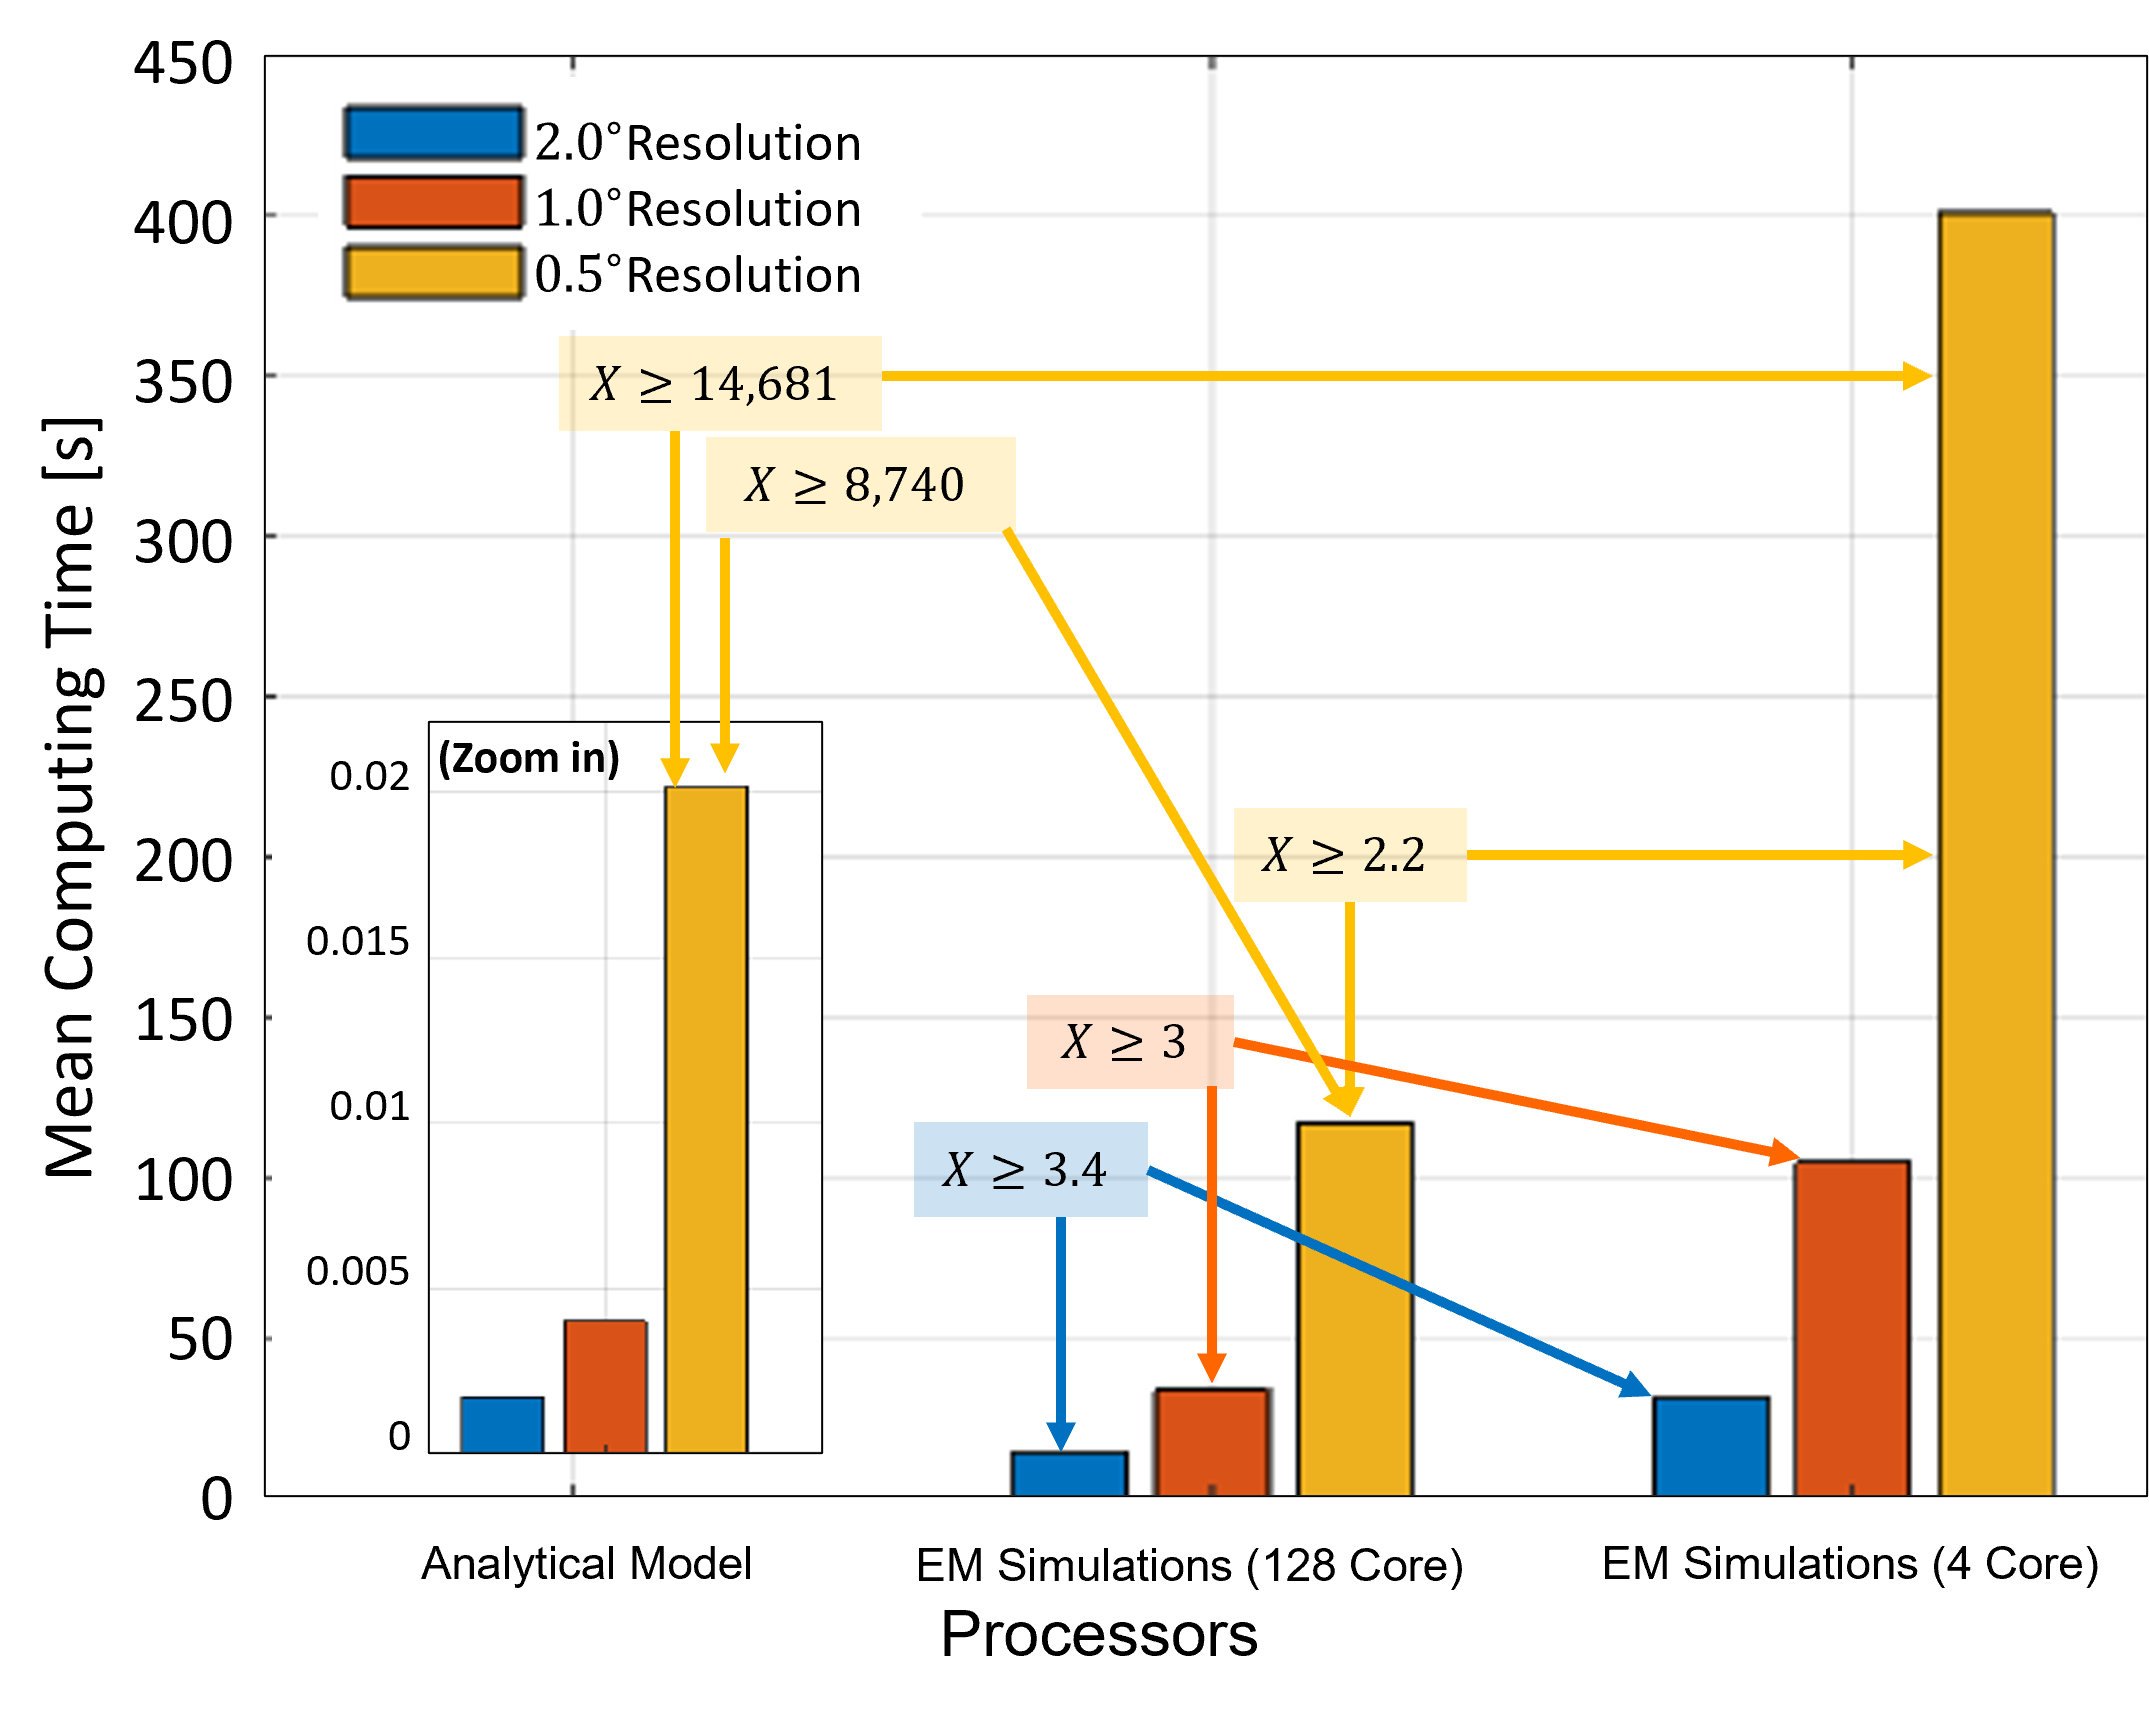
\includegraphics[width=0.75\linewidth]{images/Section 4 Images/Computing_time_cores}
	\caption{Mean computing time for a HELIOS module with different angular resolutions focusing on the speed-up factor X between different processors. Here, we find that the analytical model implementation is up to ca. $14,600$ times faster than the EM simulations with 4 core and ca. $8,740$ times faster than 128 core at $\num{0.5}^\circ$ angular resolution.}
	\label{fig:Computing_time_cores}
\end{figure}
\begin{figure}[H]
	\centering
	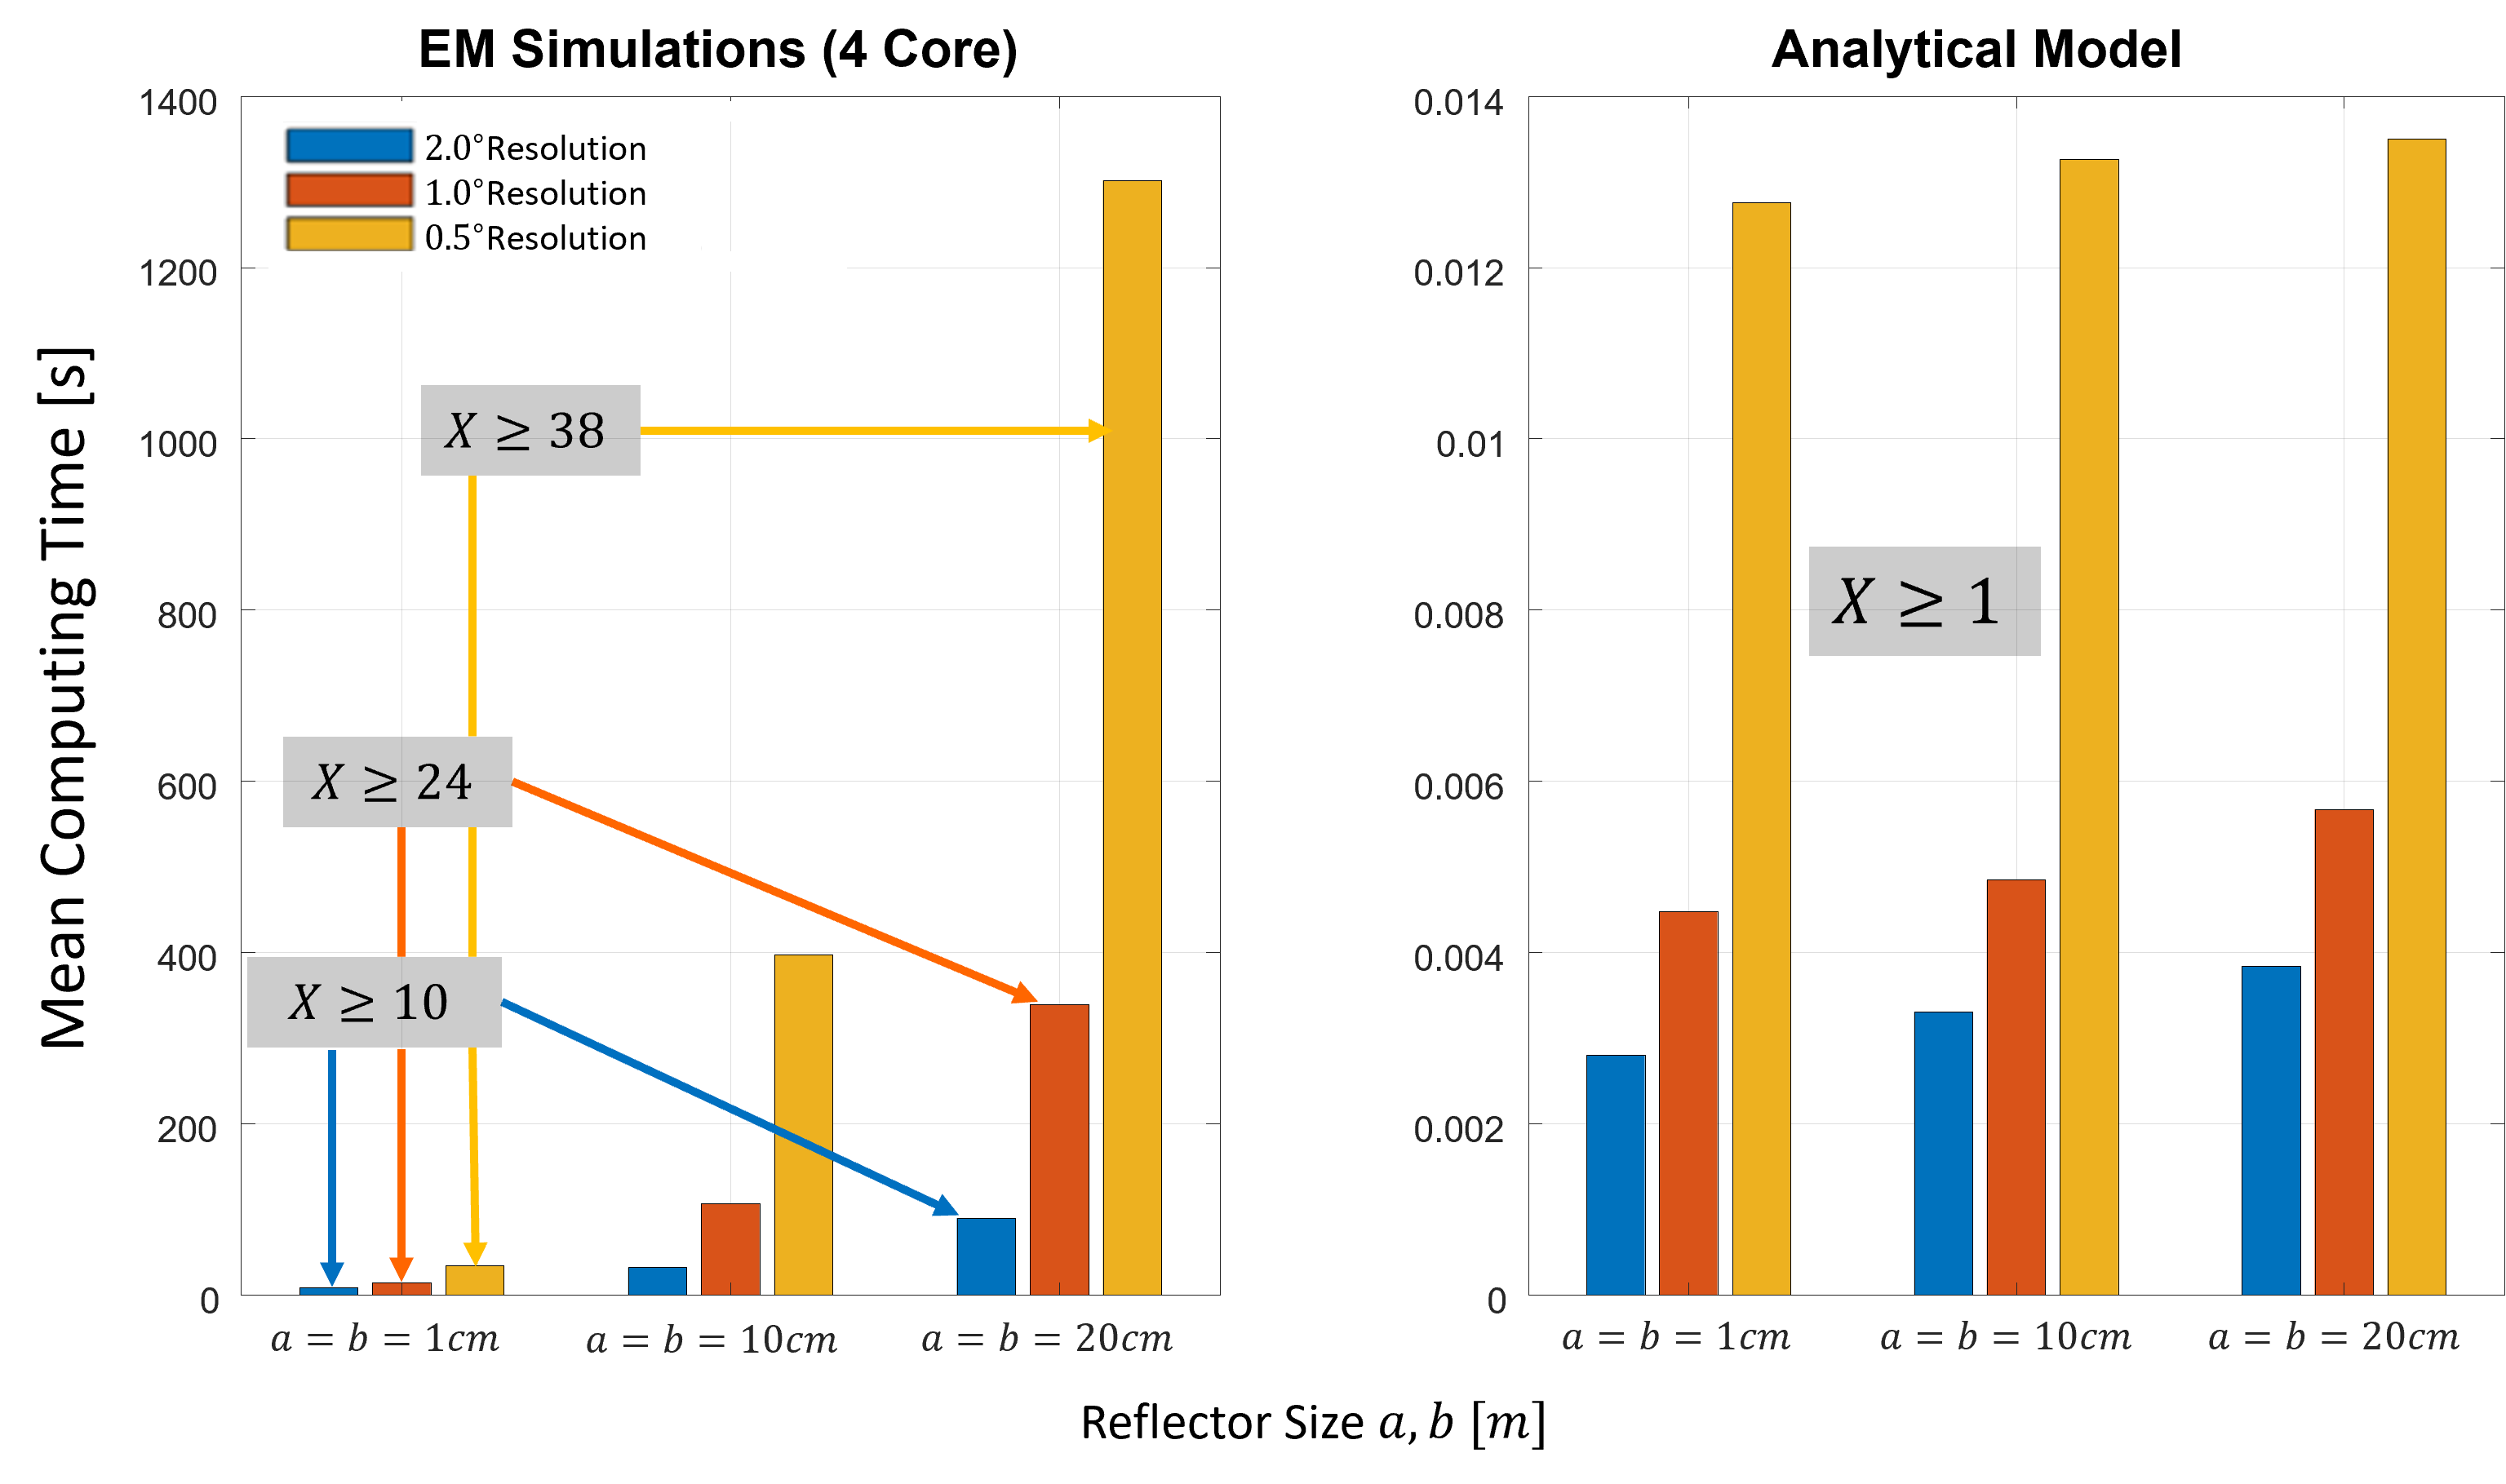
\includegraphics[width=0.85\linewidth]{images/Section 4 Images/Computing_time_size}
	\caption{Mean computing time analysis for a HELIOS module ($1 \times 1$) with varying angular resolutions highlighting the speed-up factors X between varying reflector sizes. Notably, as the reflector size increases, the mean computing time also increases in EM simulations with 4 core, but analytical model shows very little impact for varying sizes. }
	\label{fig:Computing_time_size}
\end{figure}
As can be noted, the results in \Cref{Table:Mean calculation time} corresponds to $a=b=\SI{10}{\centi\meter}$. Having considered the impact of the selected angular resolution of the RCS pattern, we move on to studying the impact of the reflector element size from $a=b=\SI{1}{\centi\meter}$ to $a=b=\SI{20}{\centi\meter}$ on the runtime. Similar to the previous paragraph, the results are provided below in \Cref{fig:Computing_time_size} and \Cref{Table:Mean calculation time2} for different HELIOS module dimensions $(1 \times 1)$.

\begin{table}[tb] % H -> dieses objekt wird genau da wo der code steht festgenagelt
	\caption{Mean computing time for different angular resolutions depicting variations for varying reflector sizes for a HELIOS module. We observe that the analytical model's computing time is independent to the reflector dimensions whereas the EM simulations scale poorly, thus demonstrating infeasibility for large reflecting surfaces size as expected for 6G, cf. case study in \Cref{Urban Case Study}.}
	\label{Table:Mean calculation time2}
	\centering
	\footnotesize
	\begin{tabular}{@{} c| >{\raggedleft\arraybackslash}p{3cm} |>{\raggedleft\arraybackslash}p{3cm} |>{\raggedleft\arraybackslash}p{3cm} @{}}	
		\multicolumn{1}{c|}{\textbf{\begin{tabular}{@{}c@{}}HELIOS Module\\ Dimensions \end{tabular}}} &
		\multicolumn{1}{c|}{\textbf{\begin{tabular}{@{}c@{}}Angular \\ Resolution \end{tabular}}} & \multicolumn{1}{c|}{\textbf{\begin{tabular}{@{}c@{}}Analytical \\ Model \end{tabular}}} &  \multicolumn{1}{c}{\textbf{\begin{tabular}{@{}c@{}}EM Simulations\\ (4 Core) \end{tabular}}} \\
		\hline
		\multirow{3}{*} \textbf{$a=b=\SI{1}{\centi\meter}$}
		& $\num{2.0}^\circ$ & \SI{2.9}{\milli\second} & \SI{8.4}{\second}  \\
		\cline{2-4}
		& $\num{1.0}^\circ$ & \SI{4.5}{\milli\second} & \SI{13.9}{\second}\\
		\cline{2-4}
		& $\num{0.5}^\circ$ & \SI{12.9}{\milli\second} & \SI{33.8}{\second}\\
		\hline
		\multirow{3}{*} \textbf{$a=b=\SI{10}{\centi\meter}$}
		& $\num{2.0}^\circ$ & \SI{3.4}{\milli\second} & \SI{31.7}{\second}  \\
		\cline{2-4}
		& $\num{1.0}^\circ$ & \SI{4.9}{\milli\second} & \SI{106.3}{\second}\\
		\cline{2-4}
		& $\num{0.5}^\circ$ & \SI{13.3}{\milli\second} & \SI{398.1}{\second} \\
		\hline
		\multirow{3}{*} \textbf{$a=b=\SI{20}{\centi\meter}$}
		& $\num{2.0}^\circ$ & \SI{3.9}{\milli\second} & \SI{89.6}{\second}  \\
		\cline{2-4}
		& $\num{1.0}^\circ$ & \SI{5.8}{\milli\second} & \SI{338.9}{\second} \\
		\cline{2-4}
		& $\num{0.5}^\circ$ & \SI{13.5}{\milli\second} & 1,309.3 \si{\second} \\
	\end{tabular}
\end{table}
A clear pattern can be observed underlining that the computing time of the EM simulations increased in tandem with reflector size. A significant speedup factor is seen in the bar graph of the \num{4}-core simulation as the reflector size increases from $a=b=\SI{1}{\centi\meter}$ to \SI{20}{\centi\meter}. In particular, there is a speedup factor of about \num{38}, \num{24}, and \num{10} for $\num{0.5}^\circ$, $\num{1}^\circ$, and $\num{2}^\circ$ resolutions, respectively. In contrast, we observe none of this for the analytical model, i.e., there is barely an impact on the computing time. Noticing from \Cref{Table:Mean calculation time2}'s mean computing time values for the analytical model, where very little effect regarding reflector size is observed, whereas, on the other hand, the values rise to 1,309.3 \si{\second} at $\num{0.5}^\circ$ angular resolution with $a=b=\SI{20}{\centi\meter}$. These results highlight the efficiency benefits made possible by the analytical model in a variety of scenarios, highlighting its superiority when it comes to managing bigger reflector sizes when compared to the simulation method.
\begin{table}[H] % H -> dieses objekt wird genau da wo der code steht festgenagelt
	\caption{Mean computing time for various HELIOS reflector array sizes (\num{1}$\times$\num{1}, \num{2}$\times$\num{2}, and \num{4}$\times$\num{4}) with different angular resolutions. A notable performance of our analytical model in \si{\milli\second} for an increase in reflector array demonstrates the advantage of the model to assess large-scale HELIOS configurations as compared to the simulation models. Parameters: $a_{m,n}=b_{m,n}=\SI{10}{\centi\meter}$.}
	\label{Table:Mean calculation time array}
	\centering
	\footnotesize
	\begin{tabular}{@{} c|>{\raggedleft\arraybackslash}p{2.5cm} | >{\raggedleft\arraybackslash}p{2.5cm} |>{\raggedleft\arraybackslash}p{2.5cm} |>{\raggedleft\arraybackslash}p{2.5cm} @{}}	
		\multicolumn{1}{c|}{\textbf{\begin{tabular}{@{}c@{}}HELIOS Reflector\\ Array \end{tabular}}} &
		\multicolumn{1}{c|}{\textbf{\begin{tabular}{@{}c@{}}Angular \\ Resolution \end{tabular}}} & \multicolumn{1}{c|}{\textbf{\begin{tabular}{@{}c@{}}Analytical \\ Model \end{tabular}}} & 
		\multicolumn{1}{c|}{\textbf{\begin{tabular}{@{}c@{}}EM Simulations\\ (128 Core) \end{tabular}}}& \multicolumn{1}{c}{\textbf{\begin{tabular}{@{}c@{}}EM Simulations\\ (4 Core) \end{tabular}}} \\
		\hline
		\multirow{2}{*} \textbf{\num{1}$\times$\num{1}}
		& $\num{2.0}^\circ$ & \SI{1.6}{\milli\second} & \SI{14.9}{\second} & \SI{31.7}{\second}  \\
		\cline{2-5}
		& $\num{1.0}^\circ$ & \SI{3.9}{\milli\second} & \SI{33.5}{\second} & \SI{106.4}{\second}\\
		\hline
		\multirow{2}{*} \textbf{\num{2}$\times$\num{2}}
		& $\num{2.0}^\circ$  & \SI{2.8}{\milli\second} & \SI{20.6}{\second} & \SI{77.9}{\second} \\
		\cline{2-5}
		& $\num{1.0}^\circ$ & \SI{11.2}{\milli\second} & \SI{49.8}{\second}  & \SI{282.8}{\second}\\
		\hline
		\multirow{2}{*} \textbf{\num{4}$\times$\num{4}}
		& $\num{2.0}^\circ$  & \SI{9.9}{\milli\second} & \SI{66.4}{\second} & \SI{503.9}{\second} \\
		\cline{2-5}
		& $\num{1.0}^\circ$  & \SI{28.6}{\milli\second} & \SI{197.7}{\second} & 1,574.6 \si{\second} \\
	\end{tabular}
\end{table}
\begin{figure}[tb]
	\centering
	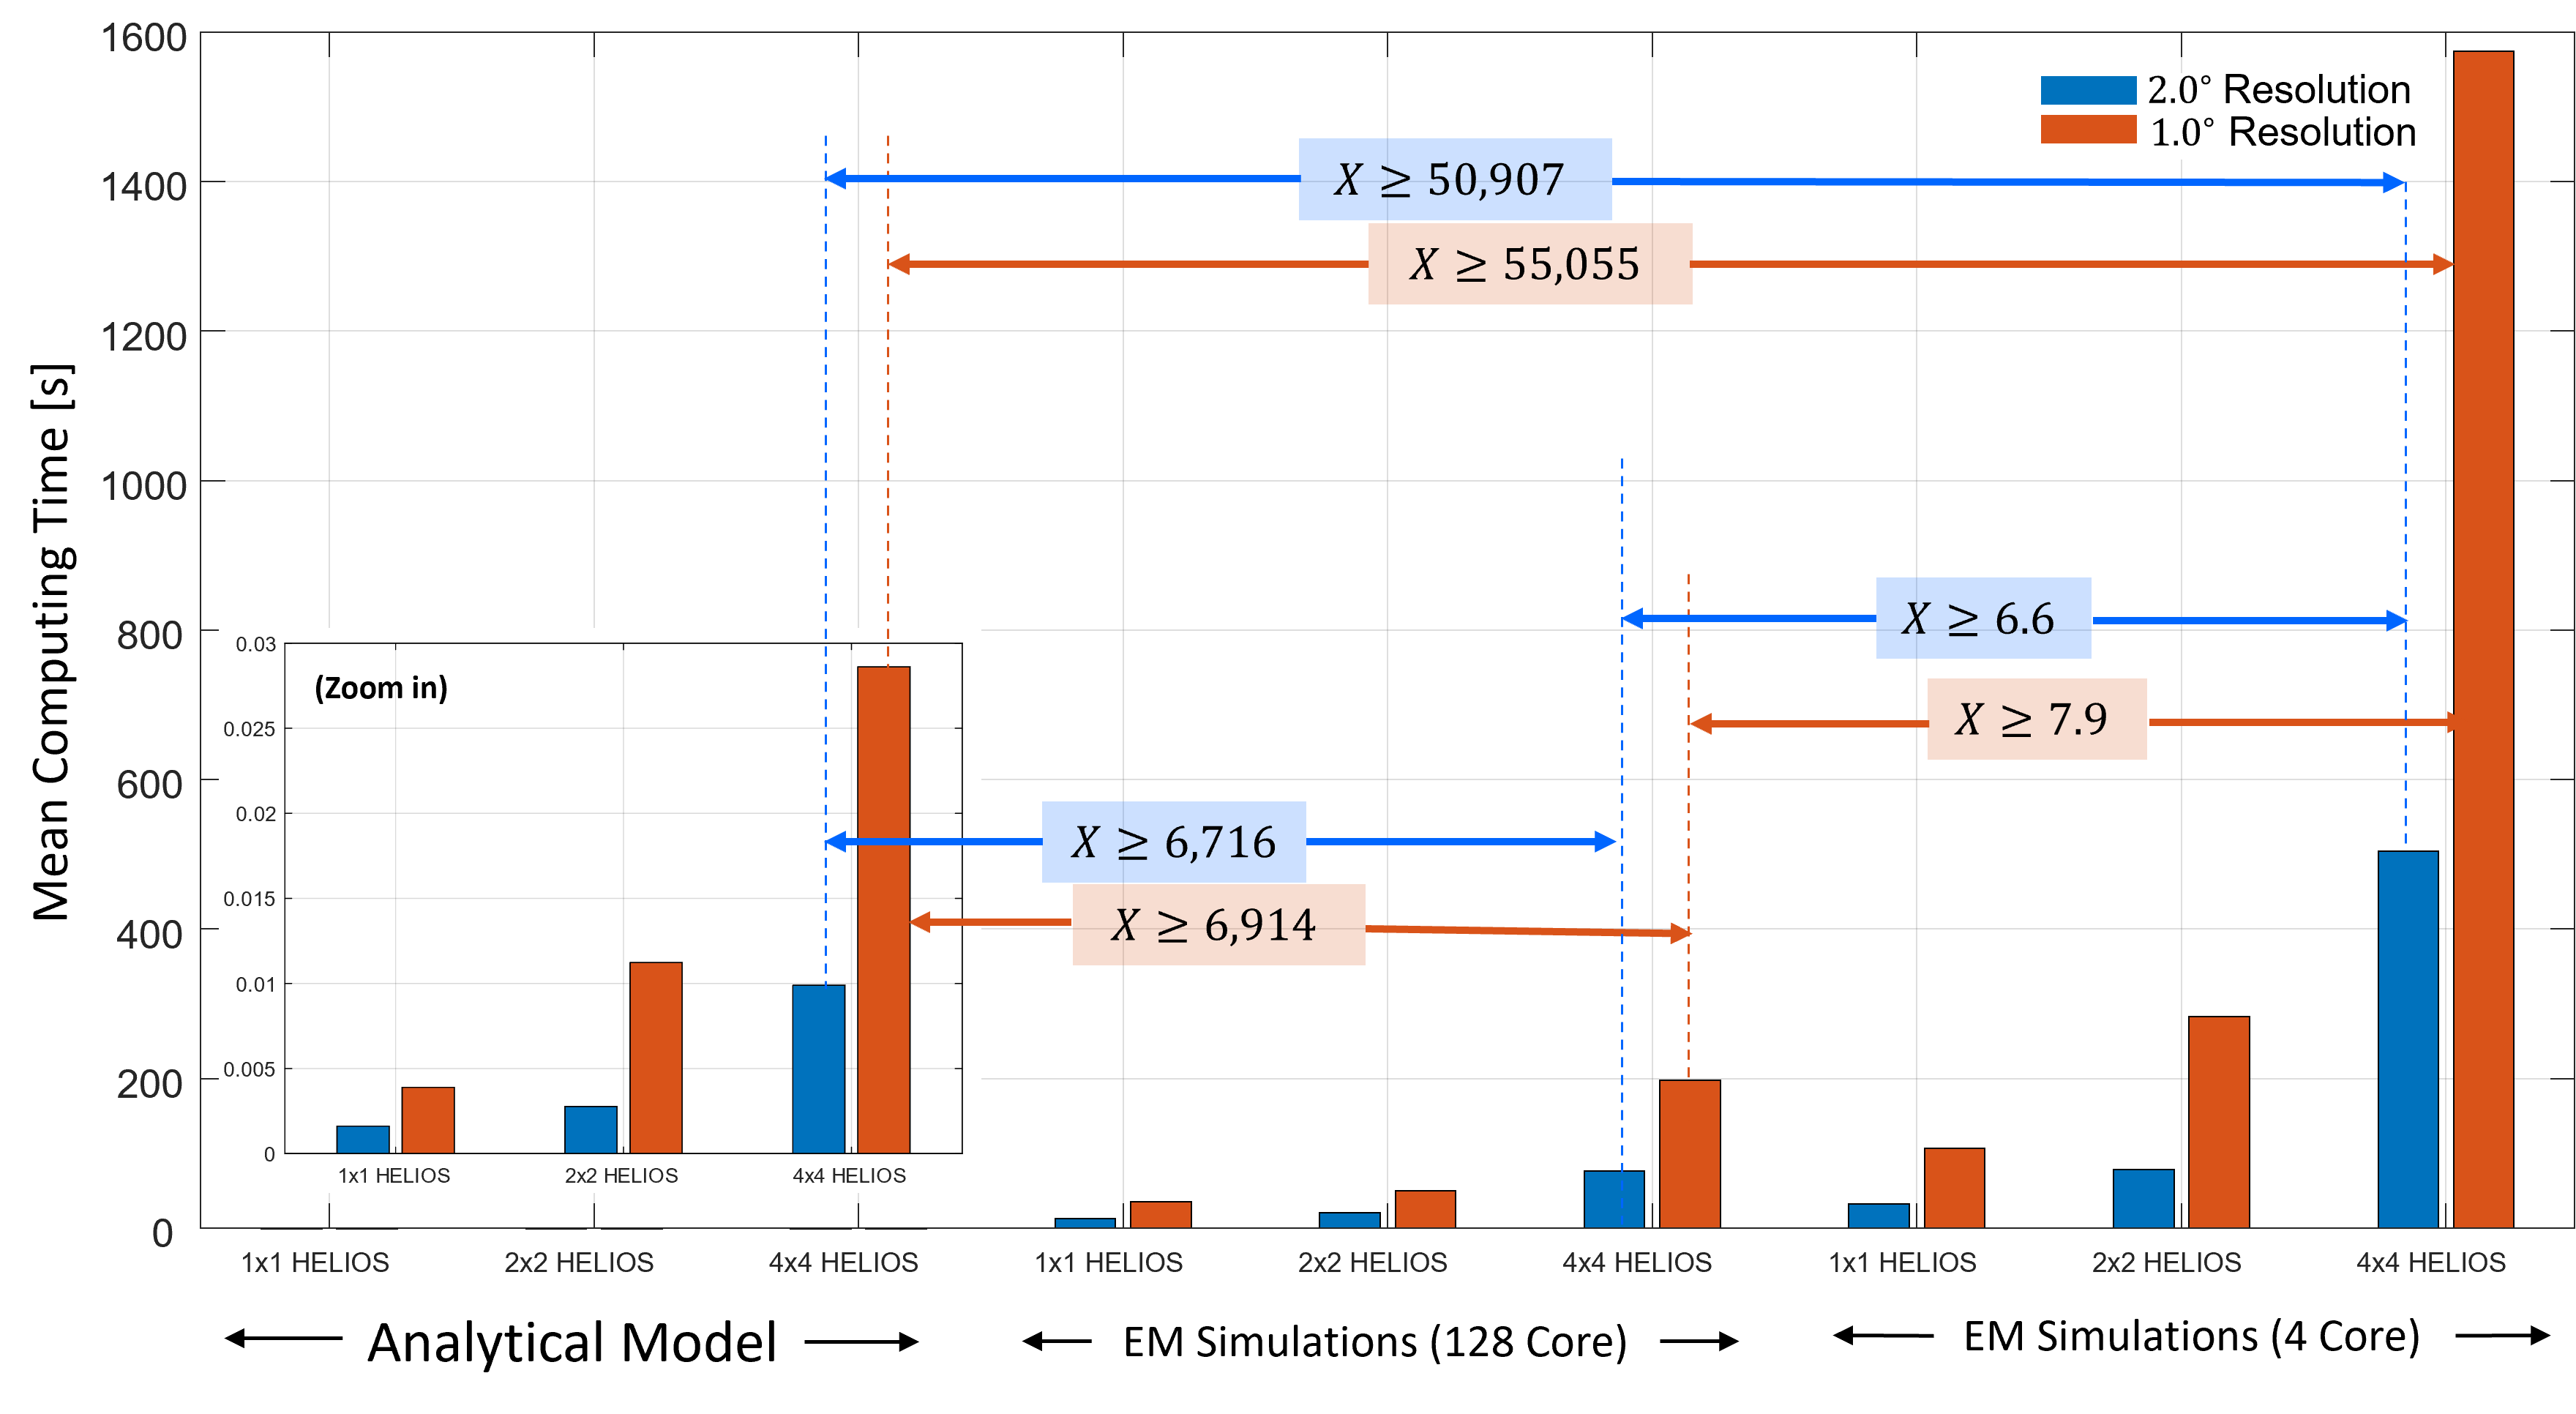
\includegraphics[width=1.0\linewidth]{images/Section 4 Images/Computing_time_resolution}
	\caption{Mean computing time analysis for various HELIOS reflector array sizes (\num{1}$\times$\num{1},\num{2}$\times$\num{2}, and \num{4}$\times$\num{4}) highlighting the speed-up factor X between different angular resolutions. A notable faster performance by the analytical model is observed for the large-scale array configurations as compared to that of the simulation model. }
	\label{fig:Computing_time_resolution}
\end{figure}
Moving on, we now investigate the computing time dynamics for various array sizes (\num{1}$\times$\num{1}, \num{2}$\times$\num{2}, and \num{4}$\times$\num{4}) using an analytical model and EM simulation of 4 core and 128 core configurations in our extended study. The mean calculation times for angular resolutions of RCS with $\num{1}^\circ$ and $\num{2}^\circ$ are given in \Cref{fig:Computing_time_resolution}, and \Cref{Table:Mean calculation time array}.  

Again, a similar pattern shows up for EM simulation architectures, indicating that computing time increases with array size. The measured speed-up factors at $\num{1}^\circ$ resolution show that the transitions from analytical model to \num{128} core EM simulations, analytical model core to \num{4} core EM simulations, and \num{128} core to \num{4} core EM simulations appear as 6,914, 55,055, and 7.9, respectively. It is interesting to note that this trend becomes stronger with decreasing angular resolution, leading to higher speedup factors. As a result, our analytical model performs substantially faster than simulation models, especially when there are a lot of array models available. This divergence highlights the efficiency boost for engineers using our proposed analytical model instead of EM simulations to assess large-scale HELIOS configurations.
\section{Urban Case Study}\label{Urban Case Study}
This section focuses on developing a deep comprehension of the urban scenario in \Cref{Urban Scenario Implementation} and forecasting various communication channel models in \Cref{Baseline Performance of FSPL Model}. By combining  the analytical model from \Cref{Analytical Modeling of HELIOS Modules} into practice in an urban setting, \Cref{Optimizing the HELIOS Geometry for Better Performance} and \Cref{Optimizing Connectivity with Different Reflector Positions} we optimize the configurations and assess the performance gains over the results with the original configurations in \Cref{Coupling Simulated and Analytical Reflection Pattern with Radar Realization}. The incorporation of this refined model into the IRS models explained in \Cref{coordinate systems} constitutes a fundamental component of our research, as seen in \Cref{Analyzing Urban Scenario for Different IRS Models}, where we also discuss two cases: beamformed to every possible position vs. one model which supports this fixed configuration similar to a passive reflector. A comparison study is carried out along with several case studies to thoroughly assess these models. Our investigation of the analytical model's effectiveness in actual urban communication situations is strengthened and expanded by these case studies. Lastly, in \Cref{Interpreting Different Channel Models} we extend our study to explore different channel models and analyze the performance gain.
\subsection{Urban Scenario Implementation}\label{Urban Scenario Implementation}
With this case study, we show how our HELIOS analytical model might be used in practice, for example in an urban environment, as shown in \Cref{fig:Scenario1}. The figure illustrates the location of the base station and clearly shows the distinction between Line-of-Sight (green-colored) and Non-Line-of-Sight (red-colored) zones. The two zones will be evaluated in \Cref{Baseline Performance of FSPL Model}. The judicious installation of a reflector on a nearby wall appears to be a good method to improve signal propagation and overcome potential obstructions in NLOS environments, as studied in \Cref{Coupling Simulated and Analytical Reflection Pattern with Radar Realization} and \Cref{Optimizing the HELIOS Geometry for Better Performance}.
\begin{figure}[H]
	\centering
	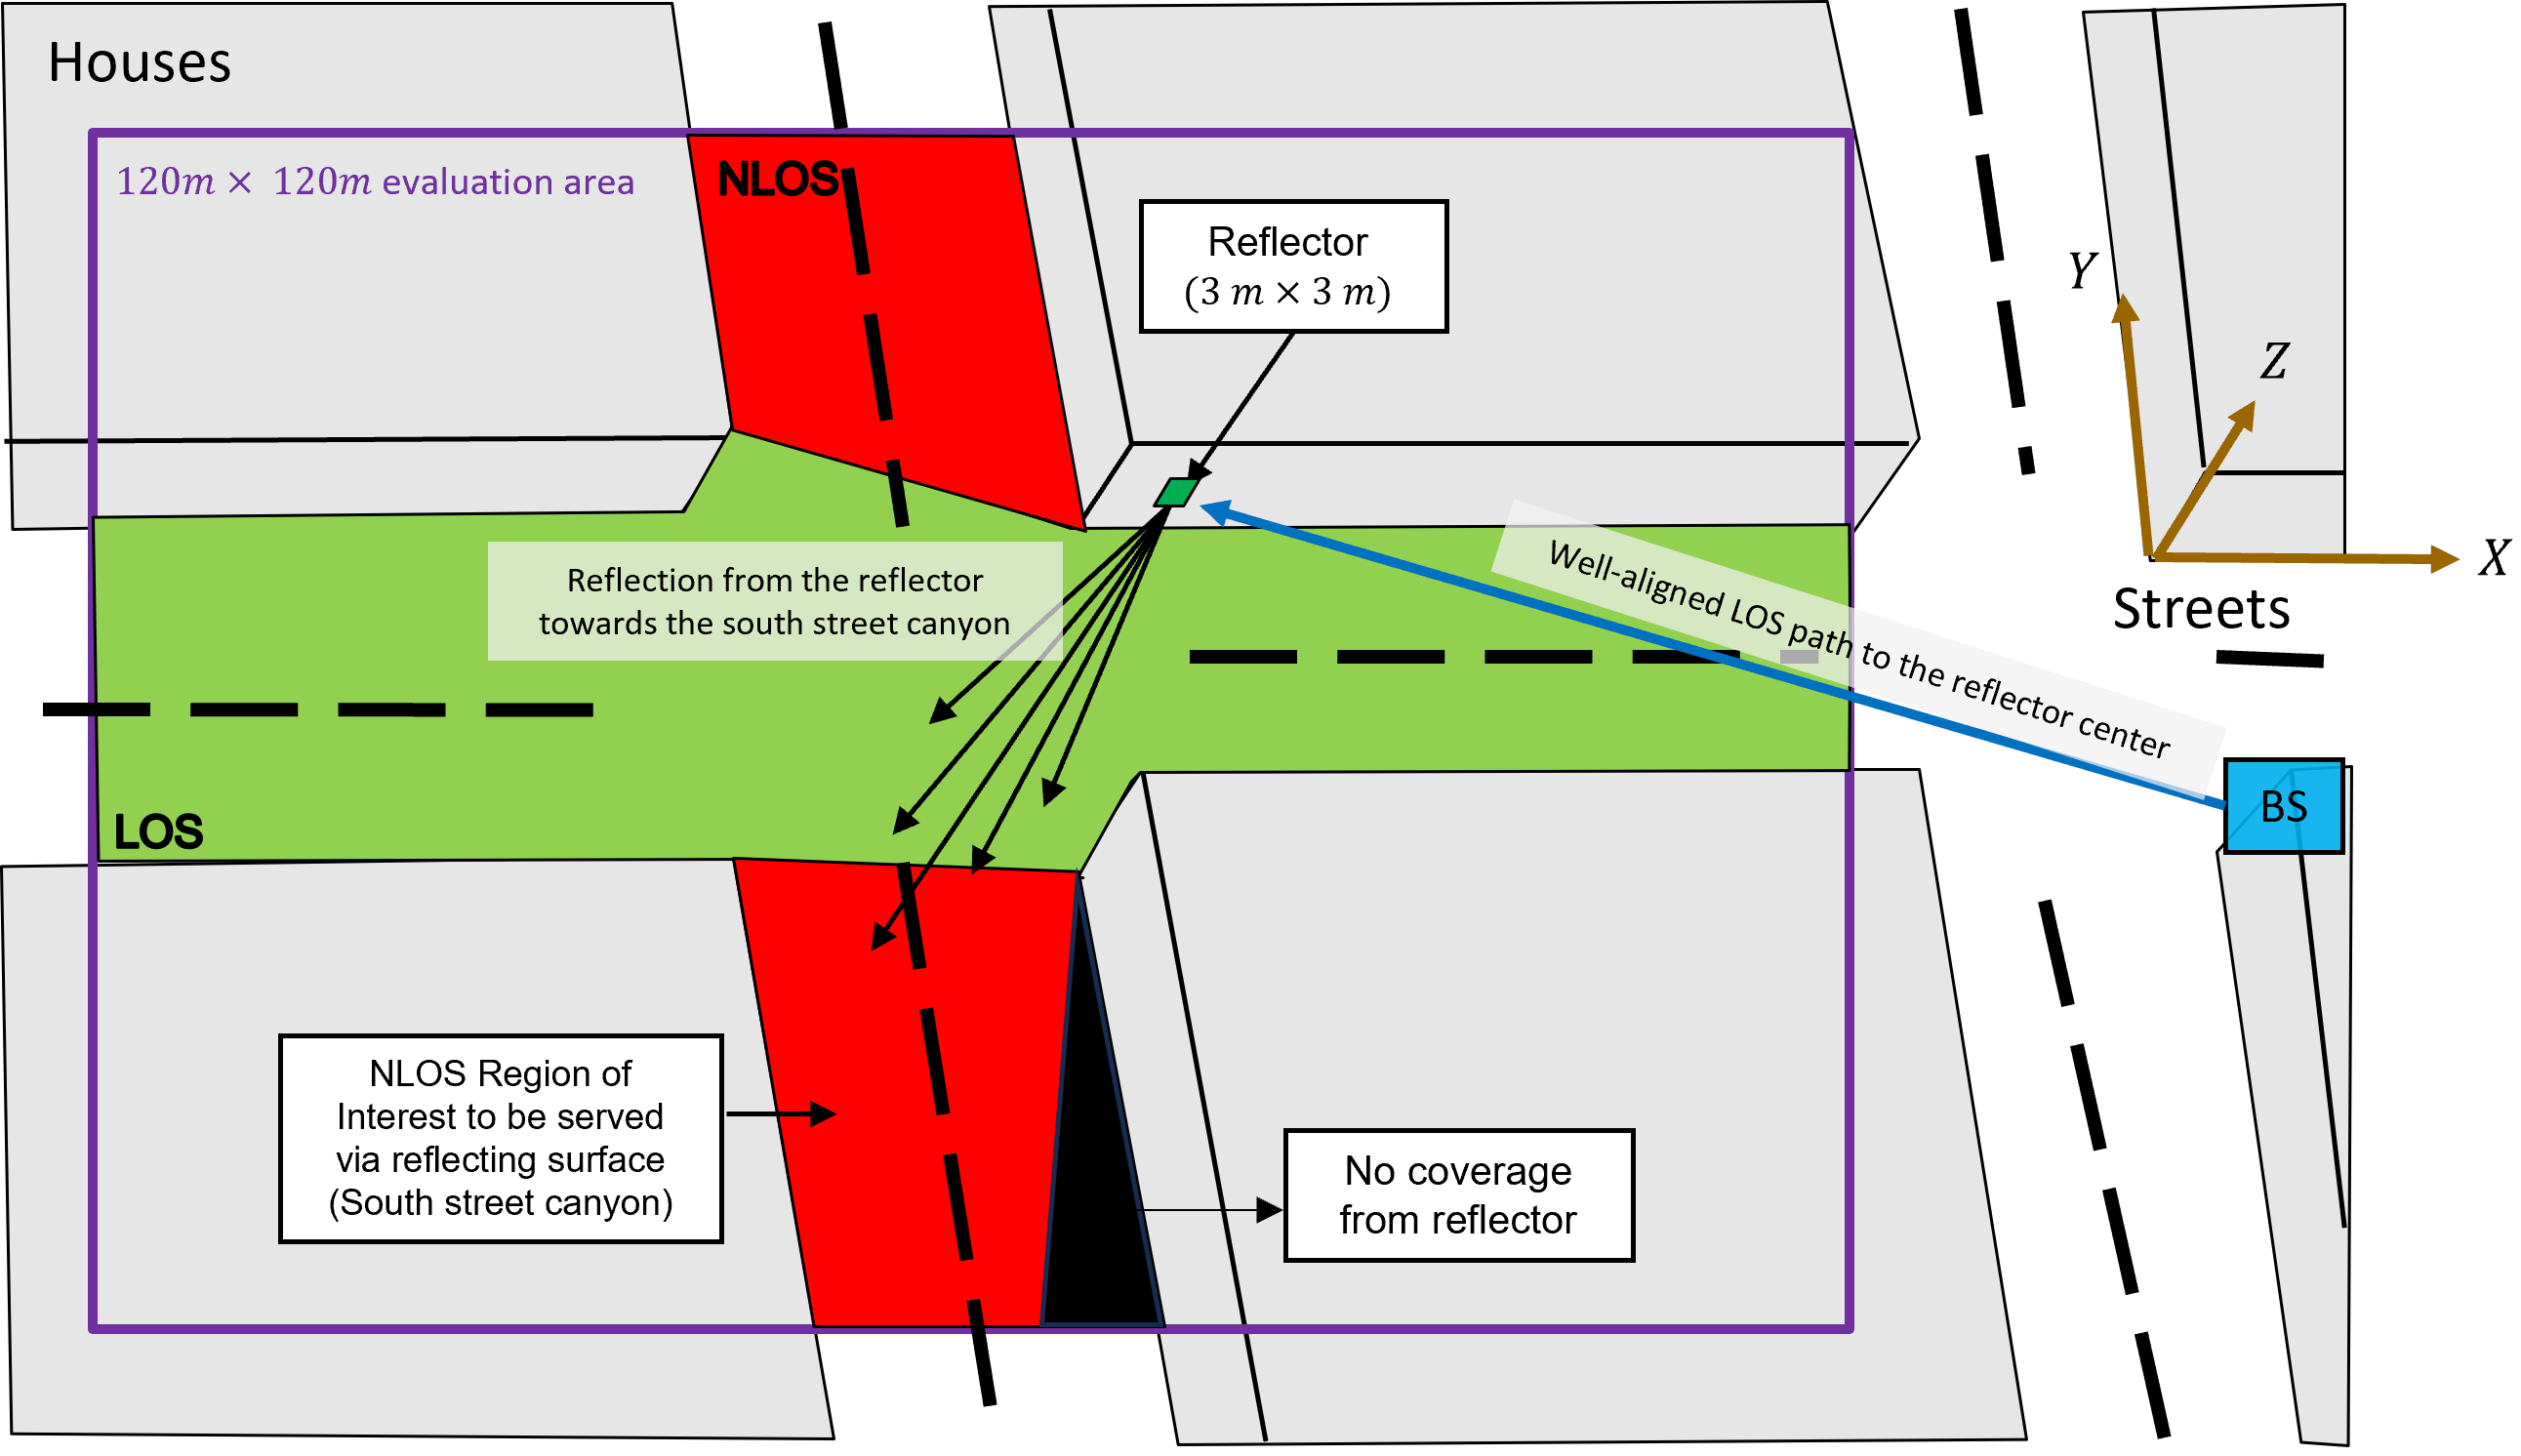
\includegraphics[width=1.0\linewidth]{images/Section 4 Images/Scenario1}
	\caption{Illustration of urban scenario \cite{Helios} with a well-aligned LOS path from the base station to the reflector center. The scenario highlights the reflections from the \SI{3}{\meter} $\times$ \SI{3}{\meter} reflector mounted on the building to serve the NLOS south street canyon region, as depicted.}
	\label{fig:Scenario1}
\end{figure}

By rerouting signals into our area of interest, i.e., south street canyon region, this reflective surface maximizes communication potential. \Cref{Table:Urban case study} provides a detailed description of the scenario's particulars, which are identical to \cite{Helios}. The base station, which uses \SI{100}{\mega\hertz} of bandwidth and operates at a frequency of \SI{28}{\giga\hertz}, is mounted on the corner of a large $ \SI{100}{\meter} \times  \SI{100}{\meter} \times \SI{20}{\meter}$ building complex at a height of \SI{10}{\meter}. According to \Cref{Table:Urban case study}, the parameters $\varphi_{BS}$ and $\theta_{BS}$ guide the orientation of the base station to precisely target the center of a designated \SI{3}{\meter} $\times$ \SI{3}{\meter}  mounting area for different reflectors under test, always mounted at a height of \SI{5}{\meter} above ground. The scenario takes place at a street crossing, where the transmitted signal from the base station is in a well-aligned LOS path to the reflector center. In a grid with \SI{1}{\meter} spacing, the receiver grid is uniformly positioned at a height of \SI{1.5}{\meter} and stretches up to \SI{60}{\meter} from the crossing point. Most notably, this simulation includes channels between the transmitter and thousands of potential receiver positions, offering a thorough grasp of the model's functionality in an actual metropolitan setting.
\begin{table}[tb] % H -> dieses objekt wird genau da wo der code steht festgenagelt
	\caption{Key parameters and their values at transmitter, receiver, and the reflector applicable to the urban street corner scenario at \SI{28}{\giga\hertz} frequency.}
	\label{Table:Urban case study}
	\centering
	\begin{tabular}{>{\centering\arraybackslash}m{2cm}|>{\centering\arraybackslash}m{7cm}|>{\centering\arraybackslash}m{5cm}}
		& \textbf{Parameter} & \textbf{Values}\\
		\hline
		\multirow{5}{*} \textbf{$P_{Tx}$}
		& Power transmitted & \SI{20.3}{\decibel}m\\
		\cline{2-3} 
		& $G_{Tx}$ & \SI{19.7}{\decibel}i\\
		\cline{2-3}
		& Position $(x,y,z)$ & (\SI{309.9}{\meter}, \SI{170.1}{\meter}, \SI{10.0}{\meter})\\
		\cline{2-3} 
		& $r_{Tx, Ref}$ & \SI{115.0}{\meter}\\
		\cline{2-3}
		& Beam orientations $(\varphi_{BS}, \theta_{BS})$ & ($\num{80.17}^\circ,\num{-2.46}^\circ $)\\
		\hline
		\multirow{8}{*} \textbf{Receiver}
		& Antenna Gain & \SI{19.7}{\decibel}i\\
		\cline{2-3} 
		& Position grid center $(x,y,z)$  & (\SI{309.9}{\meter}, \SI{170.1}{\meter}, \SI{10.0}{\meter})\\
		\cline{2-3}
		& Grid size   $x$-$z$-plane & \SI{120.0}{\meter} $\times$ \SI{120.0}{\meter}\\
		\cline{2-3} 
		& Grid density & \SI{1.0}{\meter}\\
		\cline{2-3} 
		& $r_{Ref, Rx}$ range & [\num{3.5}: \num{102.6}] \si{\meter}\\
		\cline{2-3}
		& Receiver Sensitivity $S_{Rx}$ & \SI{-83.5}{\decibel}m\\
		\cline{2-3}
		& Angle Ranges towards street crossing/Reflector $(\varphi_{UE}, \theta_{UE})$	&$ \varphi_{Rx}:[\num{-85.6}^\circ: \num{87.3}^\circ]$ and
		$\theta_{Rx}:[\num{-87.1}^\circ : \num{86.0}^\circ]$\\
		\hline
		\multirow{3}{*} \textbf{Reflector}
		& Footprint size $x$-$z$-plane & \SI{3.0}{\meter} $\times$ \SI{3.0}{\meter}\\
		\cline{2-3} 
		& Reflector Array Configuration & \num{1} $\times$ \num{32}\\
		\cline{2-3}
		& Midpoint of Reflector Backplane  $(x,y,z)$ & (\SI{195.0}{\meter}, \SI{170.0}{\meter}, \SI{5.0}{\meter})\\
	\end{tabular}
\end{table}
One thing to notice in the example is that there is a black area that is not expected to be covered via the reflector. A case study in \Cref{Optimizing Connectivity with Different Reflector Positions} will assess the impact of moving away from the reflector mounting position used in the paper \cite{Helios}.

After an initial assessment of the mmWave connectivity around the street crossing in \Cref{Urban Case Study}, the connectivity gains of two HELIOS reflector deployments are considered in this section. Like in the original paper, a "narrow beam" HELIOS configuration with slope angles being constant, constitutes the first reflector deployment option. In contrast, the "broad beam" HELIOS configuration results from our exploration of a wider range of slope angles throughout the array. Both options are depicted in \Cref{fig:beams}. The two cases are described as such:
\begin{itemize}
	\item \textbf{Narrow beam HELIOS}: Slope $\alpha_{1}=...=\alpha_{32}=\num{27.6}^\circ$, and $\beta_{1}=...=\beta_{32}=0^\circ$.
	\item \textbf{Broad beam HELIOS}: Slope angle variation in steps of $\num{2.5}^\circ$ with $\alpha_{1},....,\alpha_{32} \in [17.6^\circ:32.6^\circ]$, $\alpha_{2}, \alpha_{1}= \num{17.6}^\circ$, $\alpha_{6}, ...., \alpha_{3}=  \num{20.1}^\circ$, $\alpha_{11}, ...., \alpha_{7}= \num{22.6}^\circ$, $\alpha_{17}, ...., \alpha_{12}= \num{25.1}^\circ$, $\alpha_{23}, ...., \alpha_{18}= \num{27.6}^\circ$, $\alpha_{28}, ...., \alpha_{24}= \num{30.1}^\circ$, and $\alpha_{32}, ...., \alpha_{29}= \num{32.6}^\circ$.\\
	 Similar to narrow beam reflector configuration $\beta_{1}= ...= \beta_{32}=0^\circ$.
\end{itemize}
\begin{figure}[tb]
	\centering
	\includegraphics[width=1.0\linewidth]{images/Section 4 Images/beams}
	\caption{Top view illustration of original "narrow beam" and "broad beam" configuration for \num{1} $\times$ \num{32} HELIOS. We note that due to the symmetry of the original work, we adopt the flipped indices order.}
	\label{fig:beams}
\end{figure}
The visual summary of our methodology is presented in \Cref{fig:Scenario2}, which provides a top-view portrayal of the scenario that we are studying. The outage region, or regions where the reflectors are unable to provide coverage, is depicted in \Cref{fig:Scenario2}. As in \Cref{fig:Scenario1}, the buildings are represented by gray areas. Our main goal in this illustration is to cover the area such that the received power is greater than the designated receiver sensitivity threshold, i.e., as many potential UE positions in the south street canyon shall be able to connect to the network despite being in NLOS.

\begin{figure}[H]
	\centering
	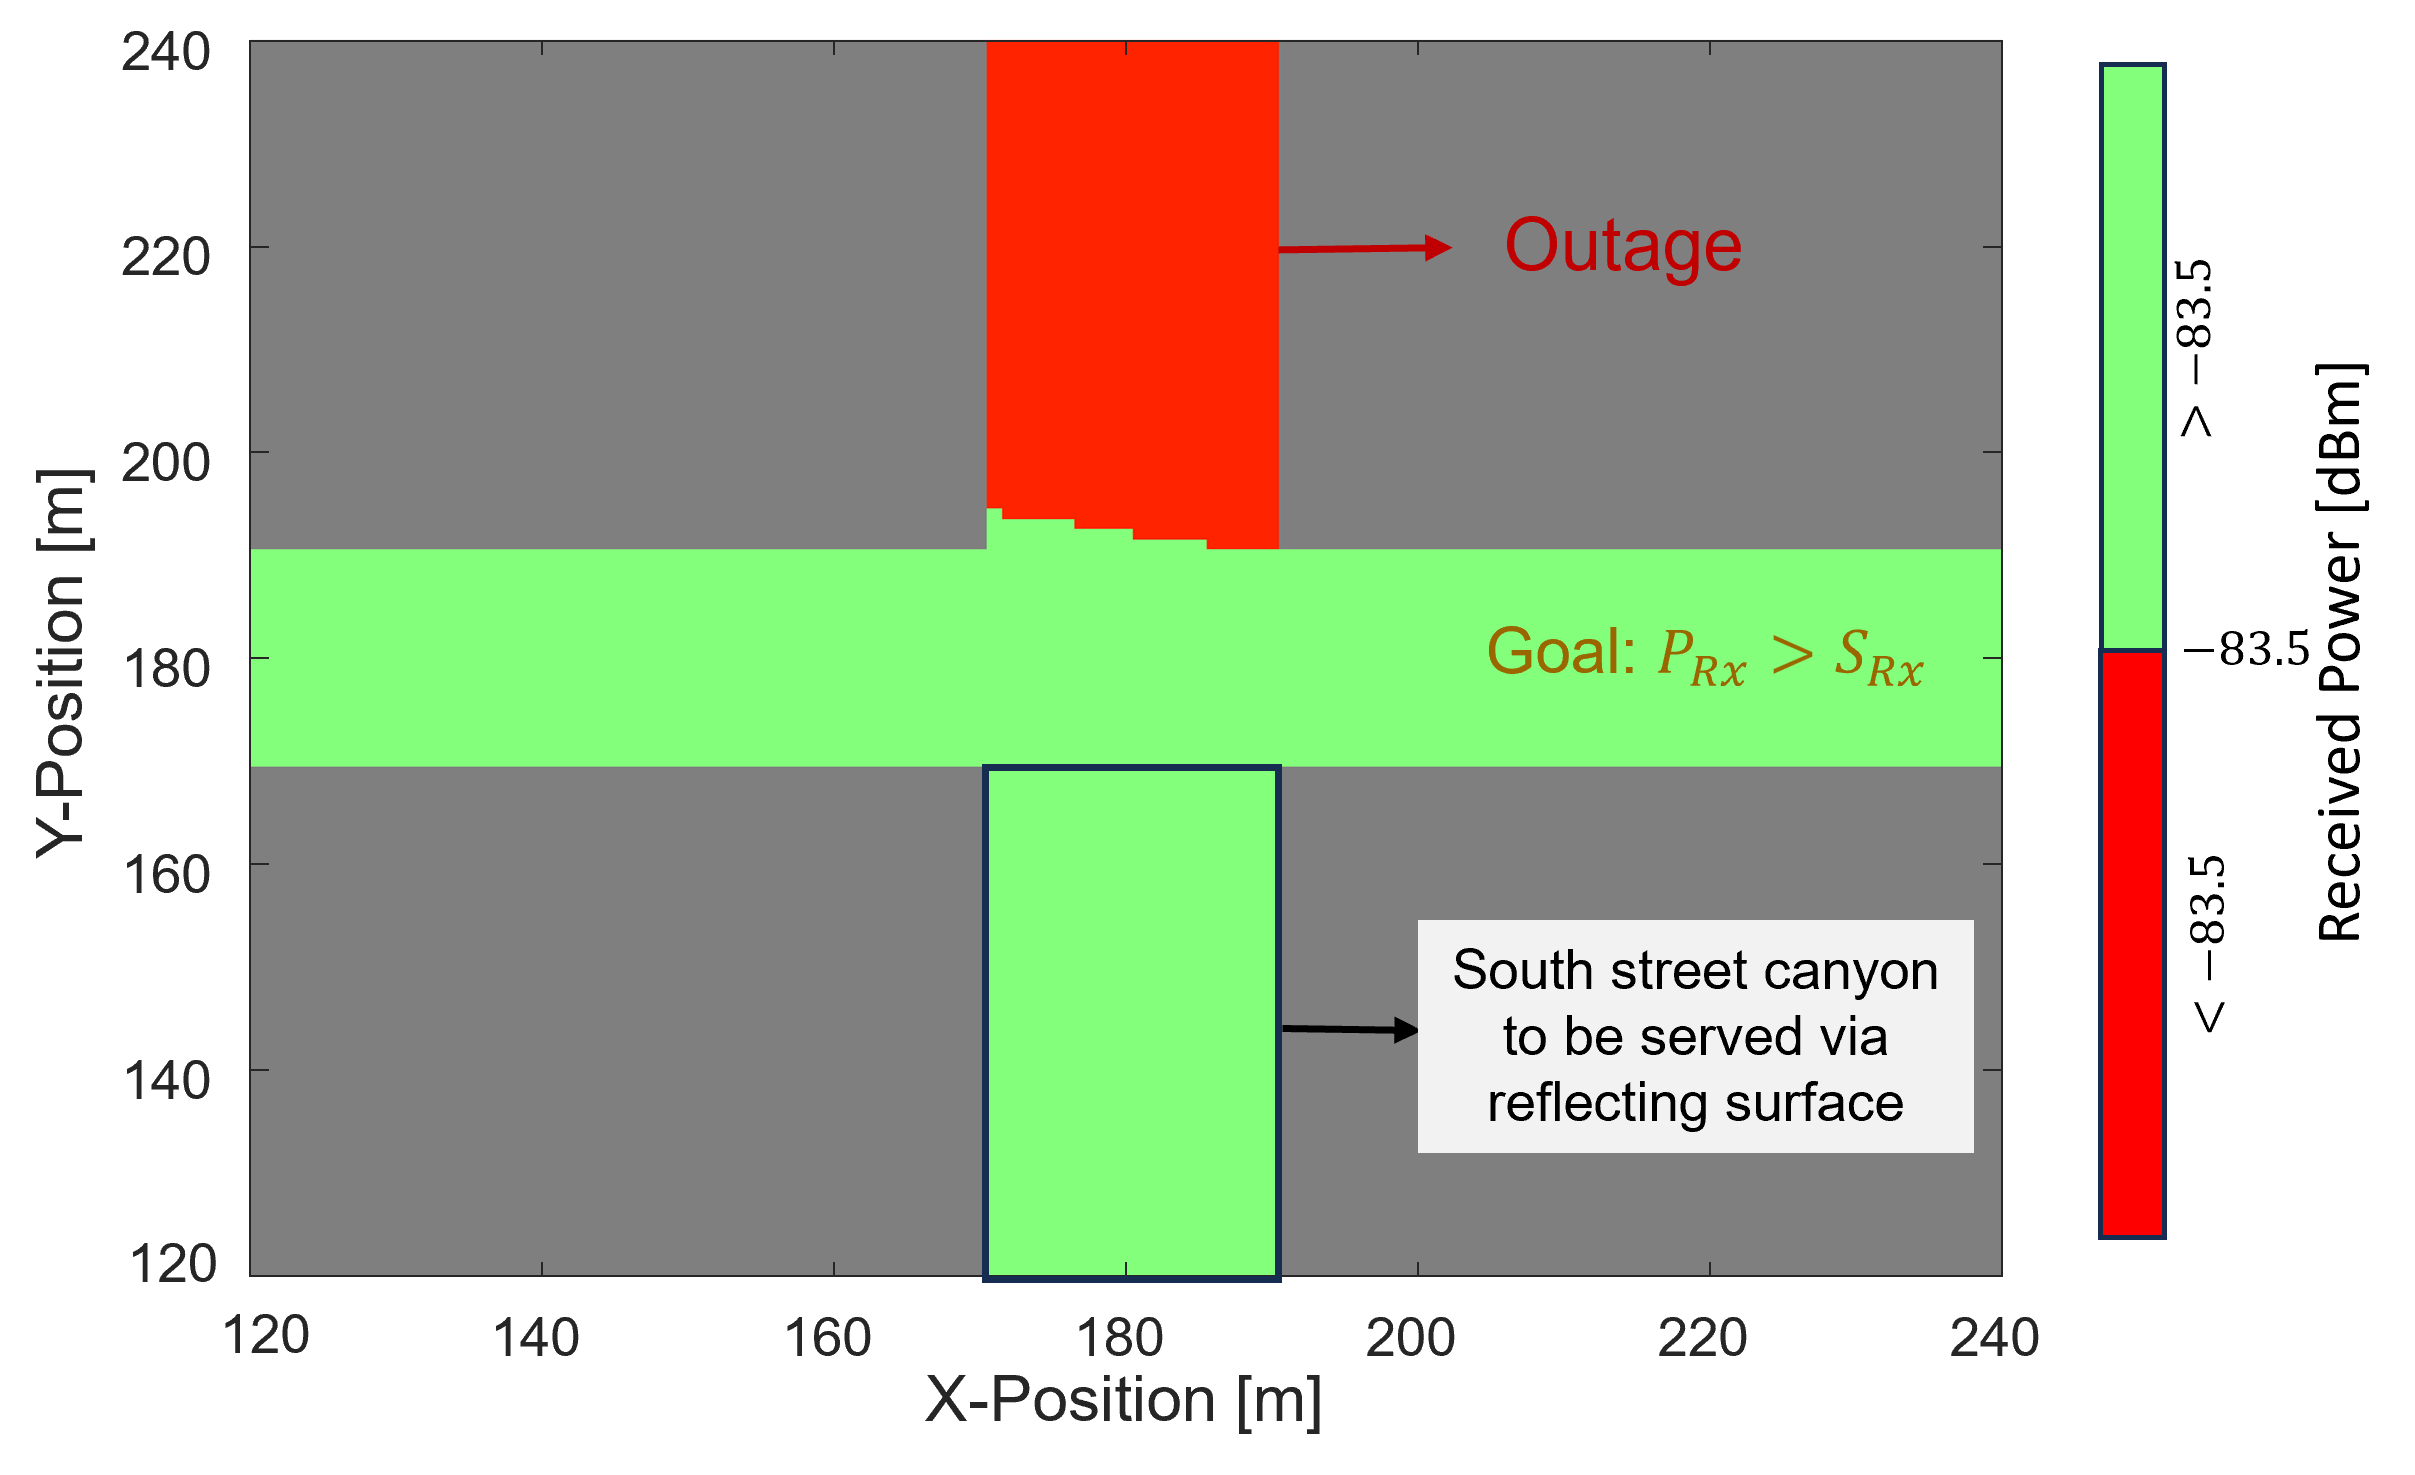
\includegraphics[width=1\linewidth]{images/Section 4 Images/Scenario2}
	\caption{Sample illustration of received power analysis in the urban scenario to highlight the region of interest, i.e., south street canyon, where received power is greater than receiver sensitivity and the outage region.}
	\label{fig:Scenario2}
\end{figure}
\subsection{Baseline Connectivity Using LOS Channel Models}\label{Baseline Performance of FSPL Model}
Here we apply the FSPL model from \Cref{Free space propagation model} to estimate the received signal strength in the LOS regions of the selected scenario. We note that the NLOS regions will be assumed to have infinite path loss. After mounting of a reflecting surface, e.g., HELIOS or IRS, we also use the radar equation \Cref{Eq:HELIOS_array} to predict the receive power level at all UE positions, i.e., NLOS and LOS positions. 

\Cref{FSPL_delta}, which represents the excess path loss components that are then removed from the comprehensive path loss equation, explains the difference between the chained path loss equations, i.e., $PL_{Tx,Ref} \circ  PL_{Ref,Rx}$ (see \Cref{FSPLChained}).  This equation provides a clear and concise illustration of the virtual LOS situation by directly representing the radar path.
\begin{equation}\label{FSPLChained}
	\begin{aligned}
		PL_{FSPL_{Radar}}(r_{Tx,Ref},r_{Ref,Rx},f,\sigma_{Meta},G_{Tx}, G_{Rx})&=PL_{FSPL}(G_{Tx}, r_{Tx,Ref},f)+PL_{FSPL}(G_{Rx}, r_{Ref,Rx},f)+\\ &\sigma_{Meta}-\Delta D_{ChainnedFSPL},
	\end{aligned}
\end{equation}
where
\begin{equation} \label{FSPL_delta}
	\Delta D_{ChainedFSPL}= 10\cdot log_{10}(4 \cdot \pi)- 20\cdot log_{10}(c)+20\cdot log_{10}(f)
\end{equation}
\Cref{FSPL_delta} is already incorporated in \Cref{FSPL_dB_Radar}. Using this equation, we refer the reader to \Cref{fig:FSPL_Radar} for a brief comparison between the power level prediction for an arbitrary scenario assuming $\sigma_{Meta}=\SI{0}{\decibel}$ and the reflector location to be $r_{Tx, Ref}=\SI{50}{\meter}$ (see \Cref{Radar-Cross-Section and Radar Equation}).
\begin{figure}[H]
	\centering
	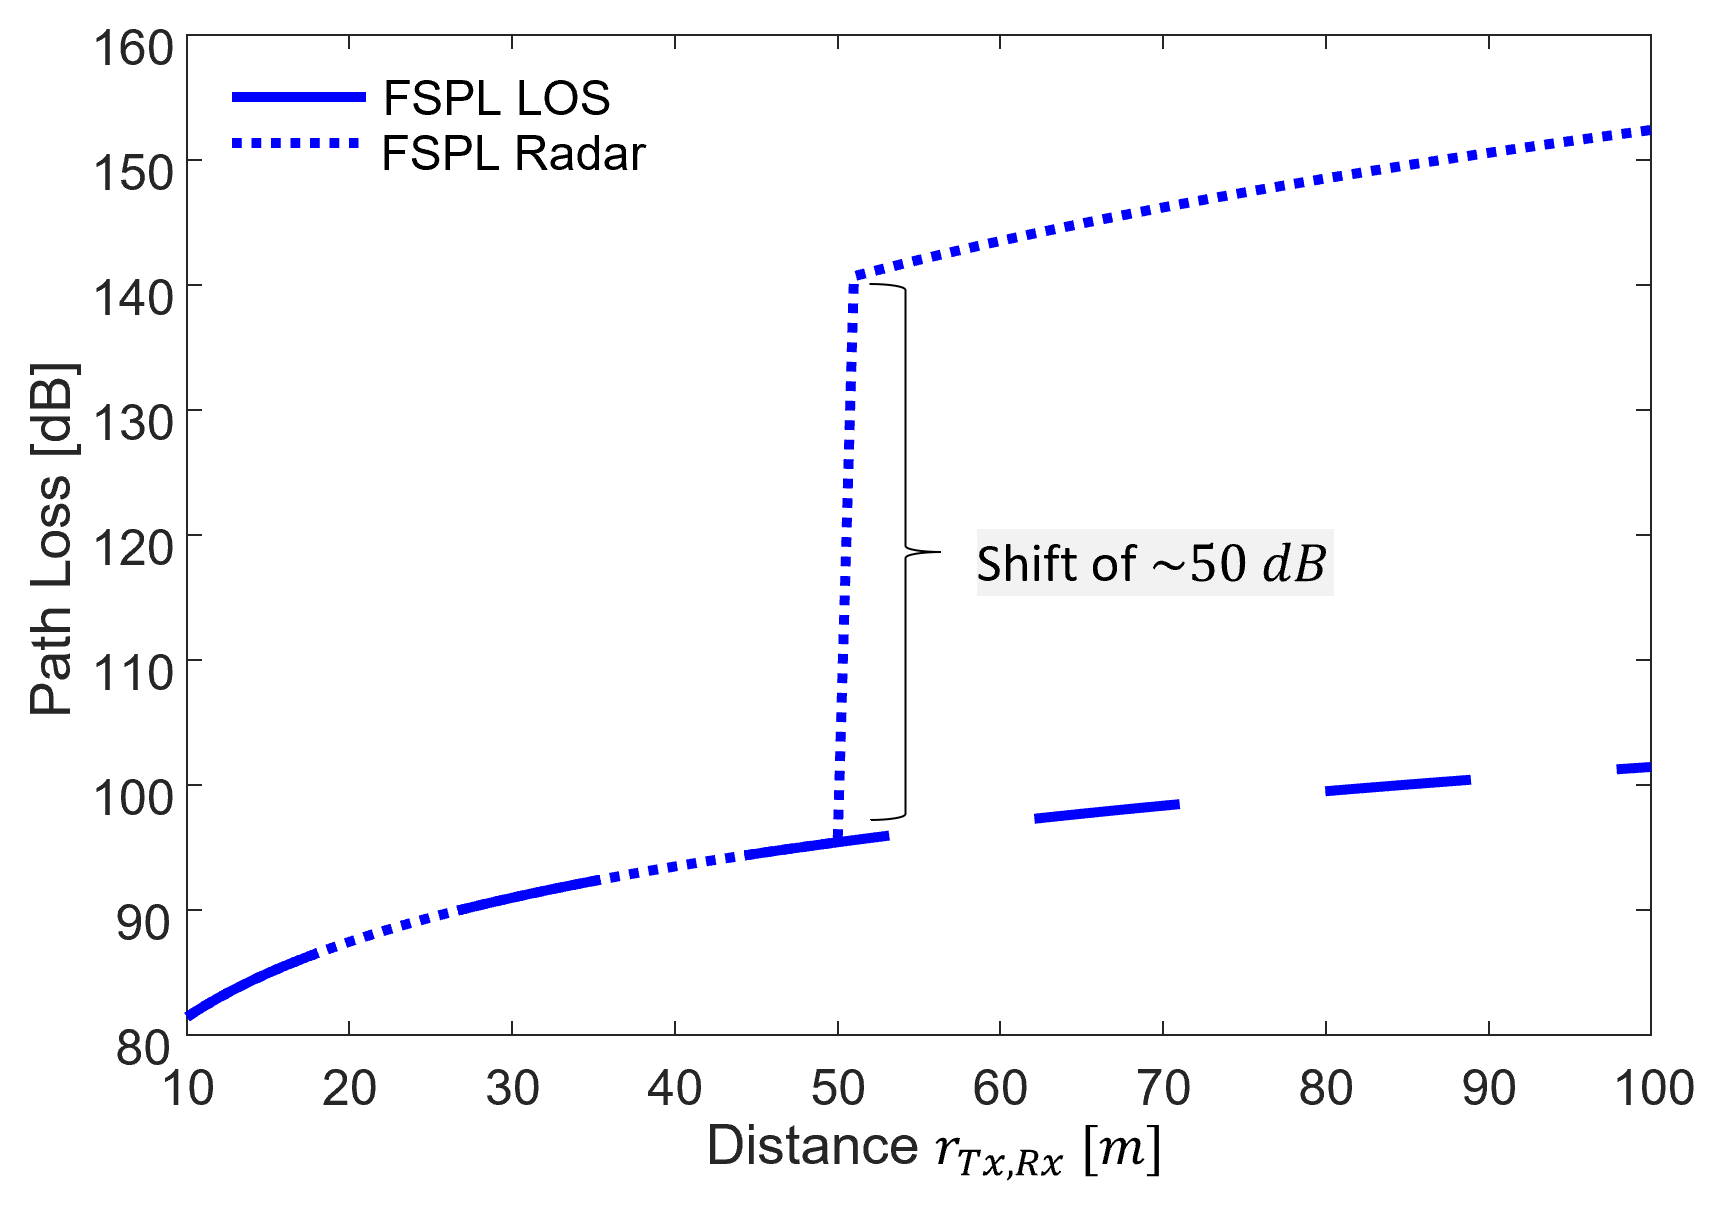
\includegraphics[width=0.75\linewidth]{images/Section 4 Images/FSPL_Radar}
	\caption{Comparison between predicted path loss of FSPL and radar equations over the total distance between Tx and Rx. For the radar equation curve, we assume LOS connectivity for the first \SI{50}{\meter}. Thereafter, it holds $\sigma_{Meta}=\SI{0}{\decibel}$, $r_{Tx, Ref}=\SI{50}{\meter}$ and $r_{Ref, Rx}=r_{Tx, Rx}$.}
	\label{fig:FSPL_Radar}
\end{figure}
A notable shift of about \SI{50}{\decibel} is observed at the reflector location $r_{Tx, Ref}=\SI{50}{\meter}$. Referring back to \Cref{Table:standard_sigma_values}, a car normally provides a $\sigma_{Meta}$ value of about \SI{20}{\decibel}. The observed shift at the reflector position is further reduced to about \SI{30}{\decibel} when considered. Using geometries explicitly tailored to achieve high RCS, such as reflecting surfaces, particularly by scaling the reflecting surface area, such scenarios as considered in the context of \Cref{fig:FSPL_Radar} can be overcome such that a reflector path can provide virtual LOS connectivity. 
\subsection{Analyzing Connectivity Enhancement by HELIOS Reflectors}\label{Coupling Simulated and Analytical Reflection Pattern with Radar Realization}
We now move on and assess the performance after mounting the narrow beam and broad beam HELIOS reflectors, respectively. For this purpose, we now put the radar equation to use, cf. \Cref{Eq:HELIOS_array}, For $\sigma_{Meta}$, we either substitute our analytical model or the simulation results, see \Cref{fig:urbanscenario_analy_sim}.

Initially, we verify the behavior of our analytical model through a comparison with simulation-based RCS patterns taken from \cite{Helios}. Our results are illustrated visually in  \Cref{fig:urbanscenario_analy_sim}, which includes heatmaps for both narrow and broad beams. The heatmaps, in particular, highlight that the coordinates $(\theta_{Rx}, \varphi_{Rx})=(\num{-2.5}^\circ, \num{-25.75}^\circ)$ are where the highest peak occurs and are in match.
\begin{figure}[H]
	\centering
	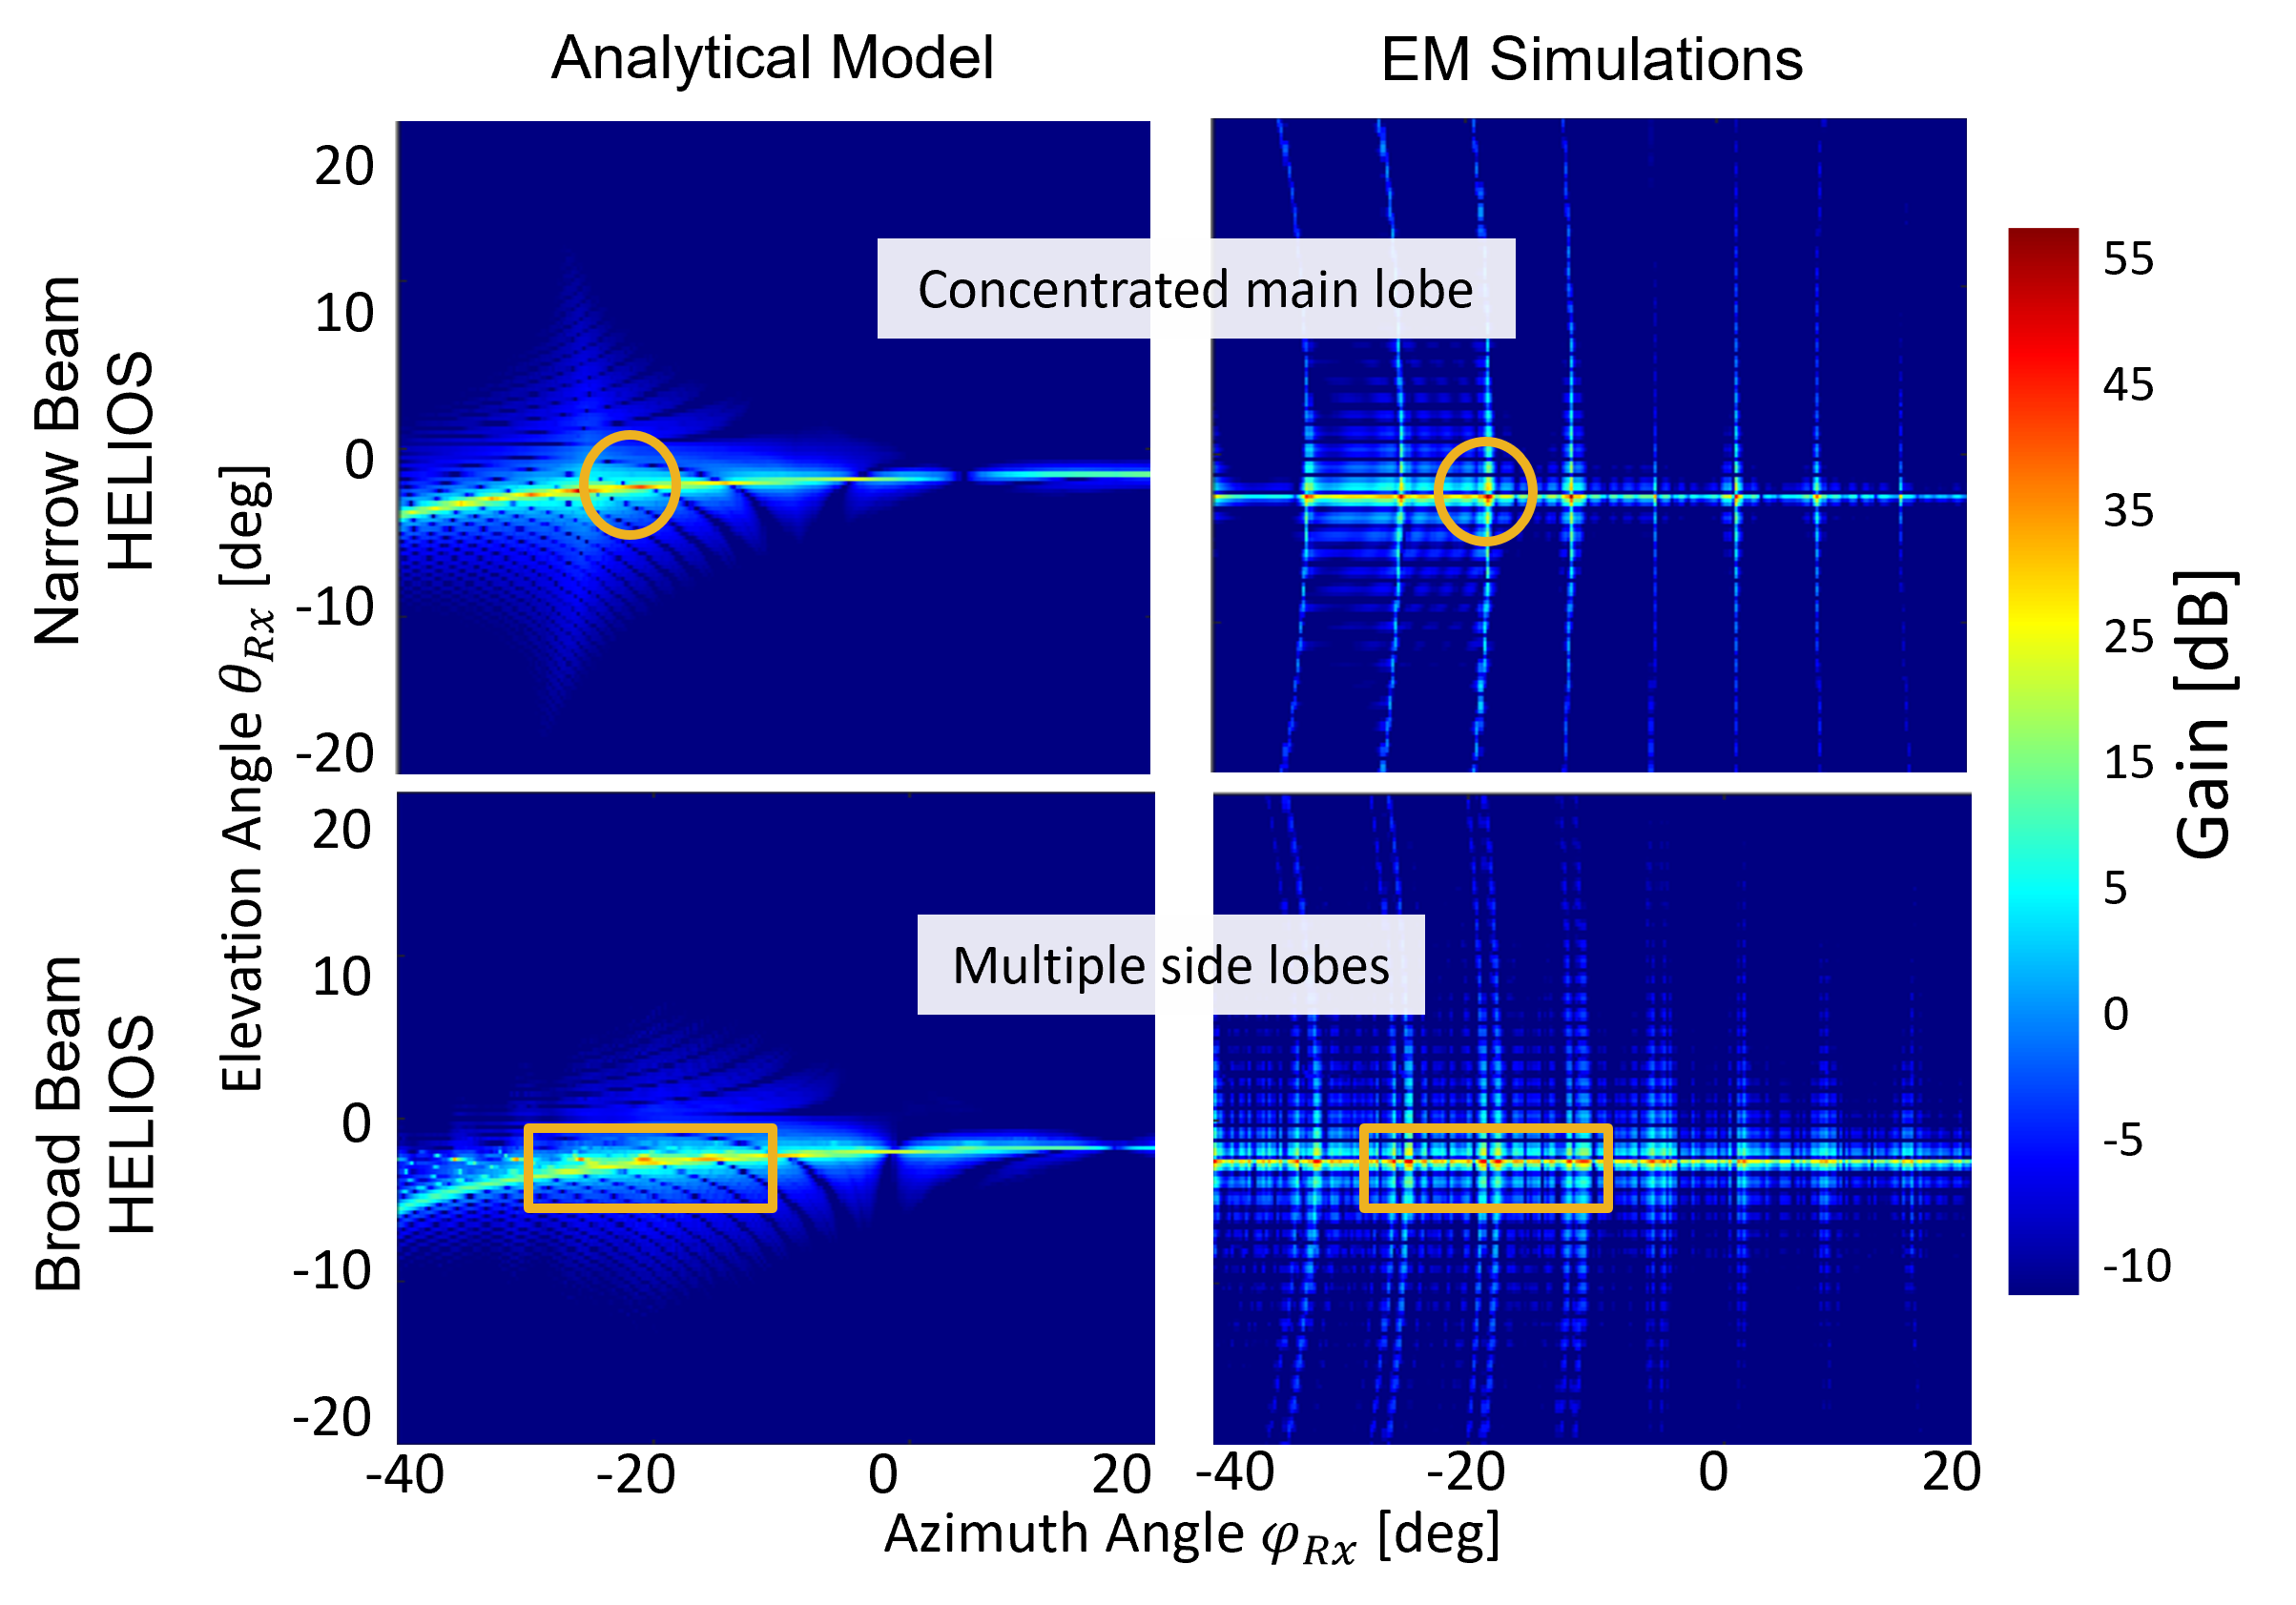
\includegraphics[width=0.9\linewidth]{images/Section 4 Images/urbanscenario_analy_sim}
	\caption{RCS comparison heatmaps between the HELIOS analytical model and EM simulation results in urban scenarios highlighting the gain behavior for both narrow and broad beams. Notably, a concentrated single lobe appears in narrow beam HELIOS, as the beams are focused in one direction at $(\theta_{Rx}, \varphi_{Rx})=(\num{-2.5}^\circ, \num{-25.75}^\circ)$, whereas with broad beam HELIOS, we observe multiple side lobes.}
	\label{fig:urbanscenario_analy_sim}
\end{figure}
The narrow beam HELIOS yields a peak gain of \SI{54.6}{\decibel} with EM simulations, whereas \SI{52.9}{\decibel} with the analytical model. Since it closely matches the simulated results, this consistency highlights the precision and dependability of our analytical method. As with broad beam HELIOS, our analytical model records a peak gain of \SI{40.7}{\decibel}, whereas the simulation model records a little higher value of \SI{48.7}{\decibel}. The overall trend shows an agreement between our analytical predictions and the simulated results, despite subtle differences in the magnitudes at the above-discussed angles. Since it faithfully reflects the simulation's observations of the larger beams' performance characteristics, this parallelism adds even more support to the validity of our analytical model.

Complementing the previous paragraph, we take a look at \Cref{fig:urbanscenario_analy_sim_ECDF} depicting the ECDFs of the previously discussed RCS heatmaps. They underline that there is a fundamental match, e.g., in terms of mean value: For the narrow beam configuration, the mean gain difference is \SI{2.8}{\decibel} with the analytical model predicting less reflection power than the EM simulations. This difference increases up to \SI{9.7}{\decibel} for the broad beam HELIOS. Whereas this suffices that the analytical model does not overpredict, we note that the ECDFs are not always weaker than the ones of the simulations. However, this shows that overprediction is rare. Like our investigation in \Cref{Analytical Modeling of HELIOS Modules}, this suggests that our analytical model provides a conservative estimate, even when scaling the reflecting surface to such large dimensions which potentially pushes analytical models and EM simulation tools to the limit.

In this section, we assess the impact on the received power for UEs located in the far-field region of the reflector under test. To make this transparent in our result figure, we highlight the near-field zone \cite{Neubauer1997, hansen1988spherical}, as defined by \Cref{Near-field} below, as a white color coding.
\begin{figure}[H]
	\centering
	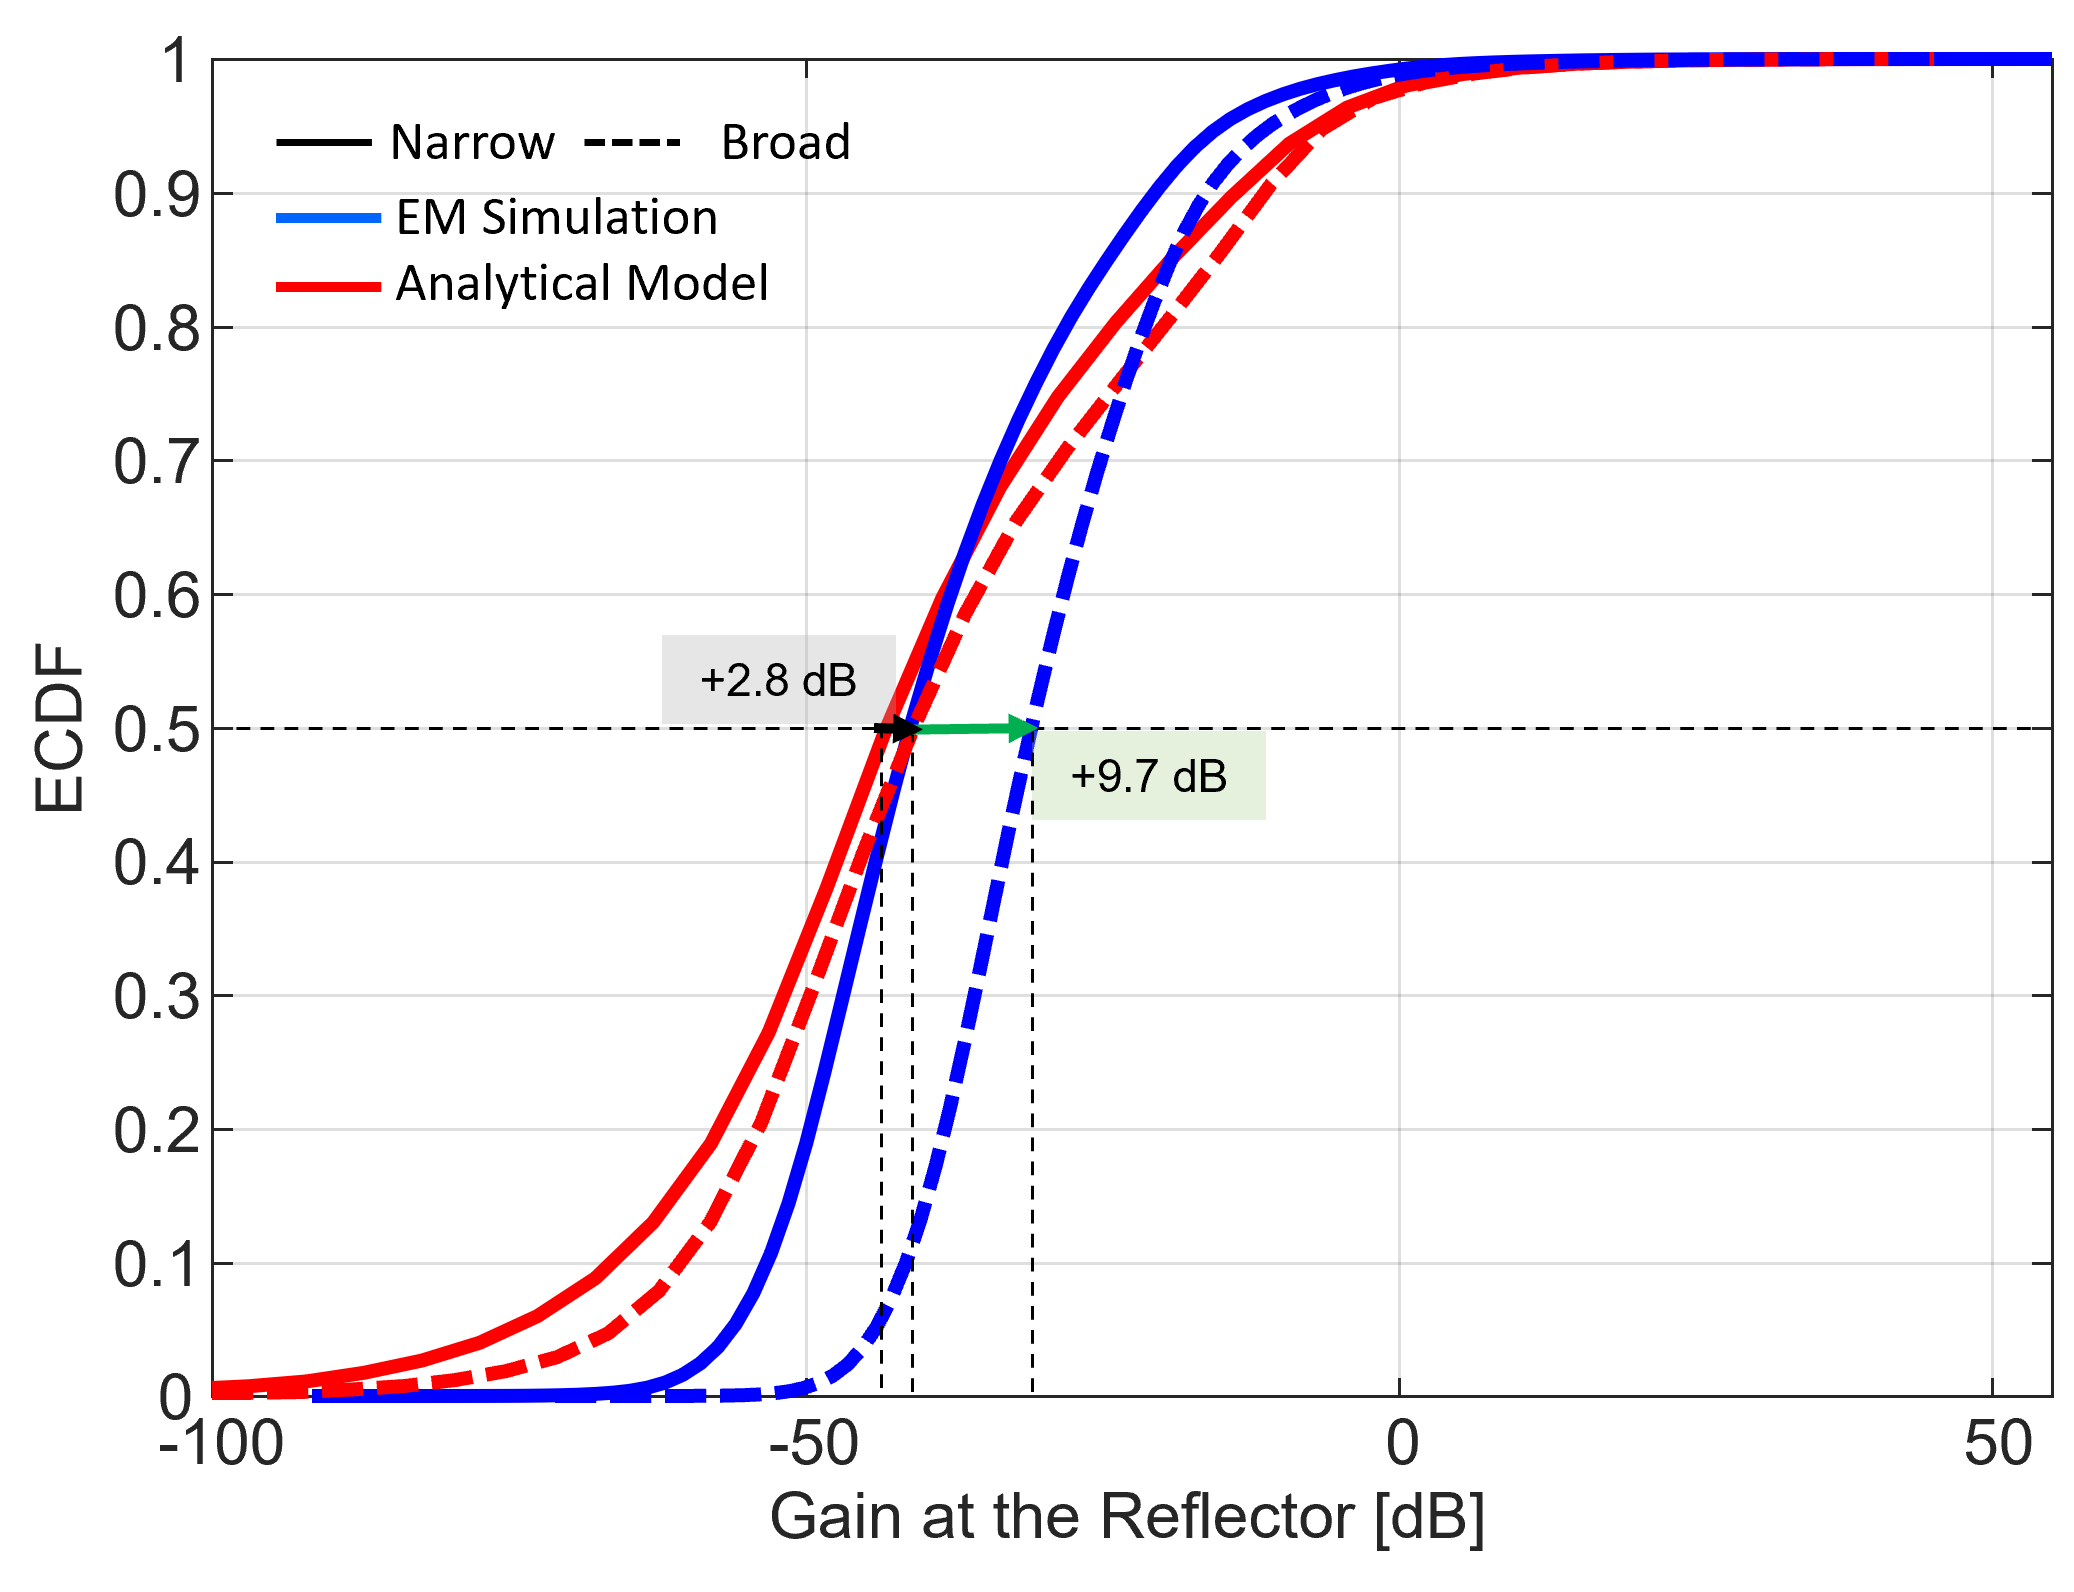
\includegraphics[width=0.7\linewidth]{images/Section 4 Images/urbanscenario_analy_sim_ECDF}
	\caption{ECDF vs gain at the reflector plot for narrow and broad beam HELIOS highlighting the difference along the mean between simulated results and analytical model in \si{\decibel}. The parameters are considered from \Cref{Table:Urban case study} at \SI{28}{\giga\hertz} frequency. }
	\label{fig:urbanscenario_analy_sim_ECDF}
\end{figure}
Given $M\cdot a=N\cdot b=\SI{3}{\meter}$, the near-field region extends up to \SI{8.4}{\meter} in this case study. 
\begin{equation} \label{Near-field}
	r_{Ref, Rx} \leq \frac{\max \left( \left( M \cdot a \right)^2, \left( N \cdot b \right)^2 \right)}{\lambda}
\end{equation}
By integrating the HELIOS analytical model into our urban environment, we can predict the RCS towards each potential UE position and therefore also determine the expected receive power level. These heatmaps in \Cref{fig:urbanscenario_originalvalues} show the maximum power received which is expressed in \si{\decibel}m and the RCS gain which is measured in \si{\decibel} from the reflector into the receiver grid. The method for calculation of maximum power received is given by $P_{Rx_{Max}}= max(P_{Rx_{LOS}}, P_{Rx_{Radar}})$, where the maximum power received with LOS and radar channel modeling is considered.

From the figure below, narrow beam HELIOS gives a peak gain of about \SI{15.4}{\decibel}, whereas \SI{11.2}{\decibel} with broad beam HELIOS. It appears from the figure that power is radiating in the direction of the south street canyon. It is interesting to note, nevertheless, that radiation in the LOS area seems to have very little effect. This observation is ascribed to the shortcomings of the maximum \ac{RSS} statistic alone, as well as the complexities of the HELIOS design.
\begin{figure}[H]
	\centering
	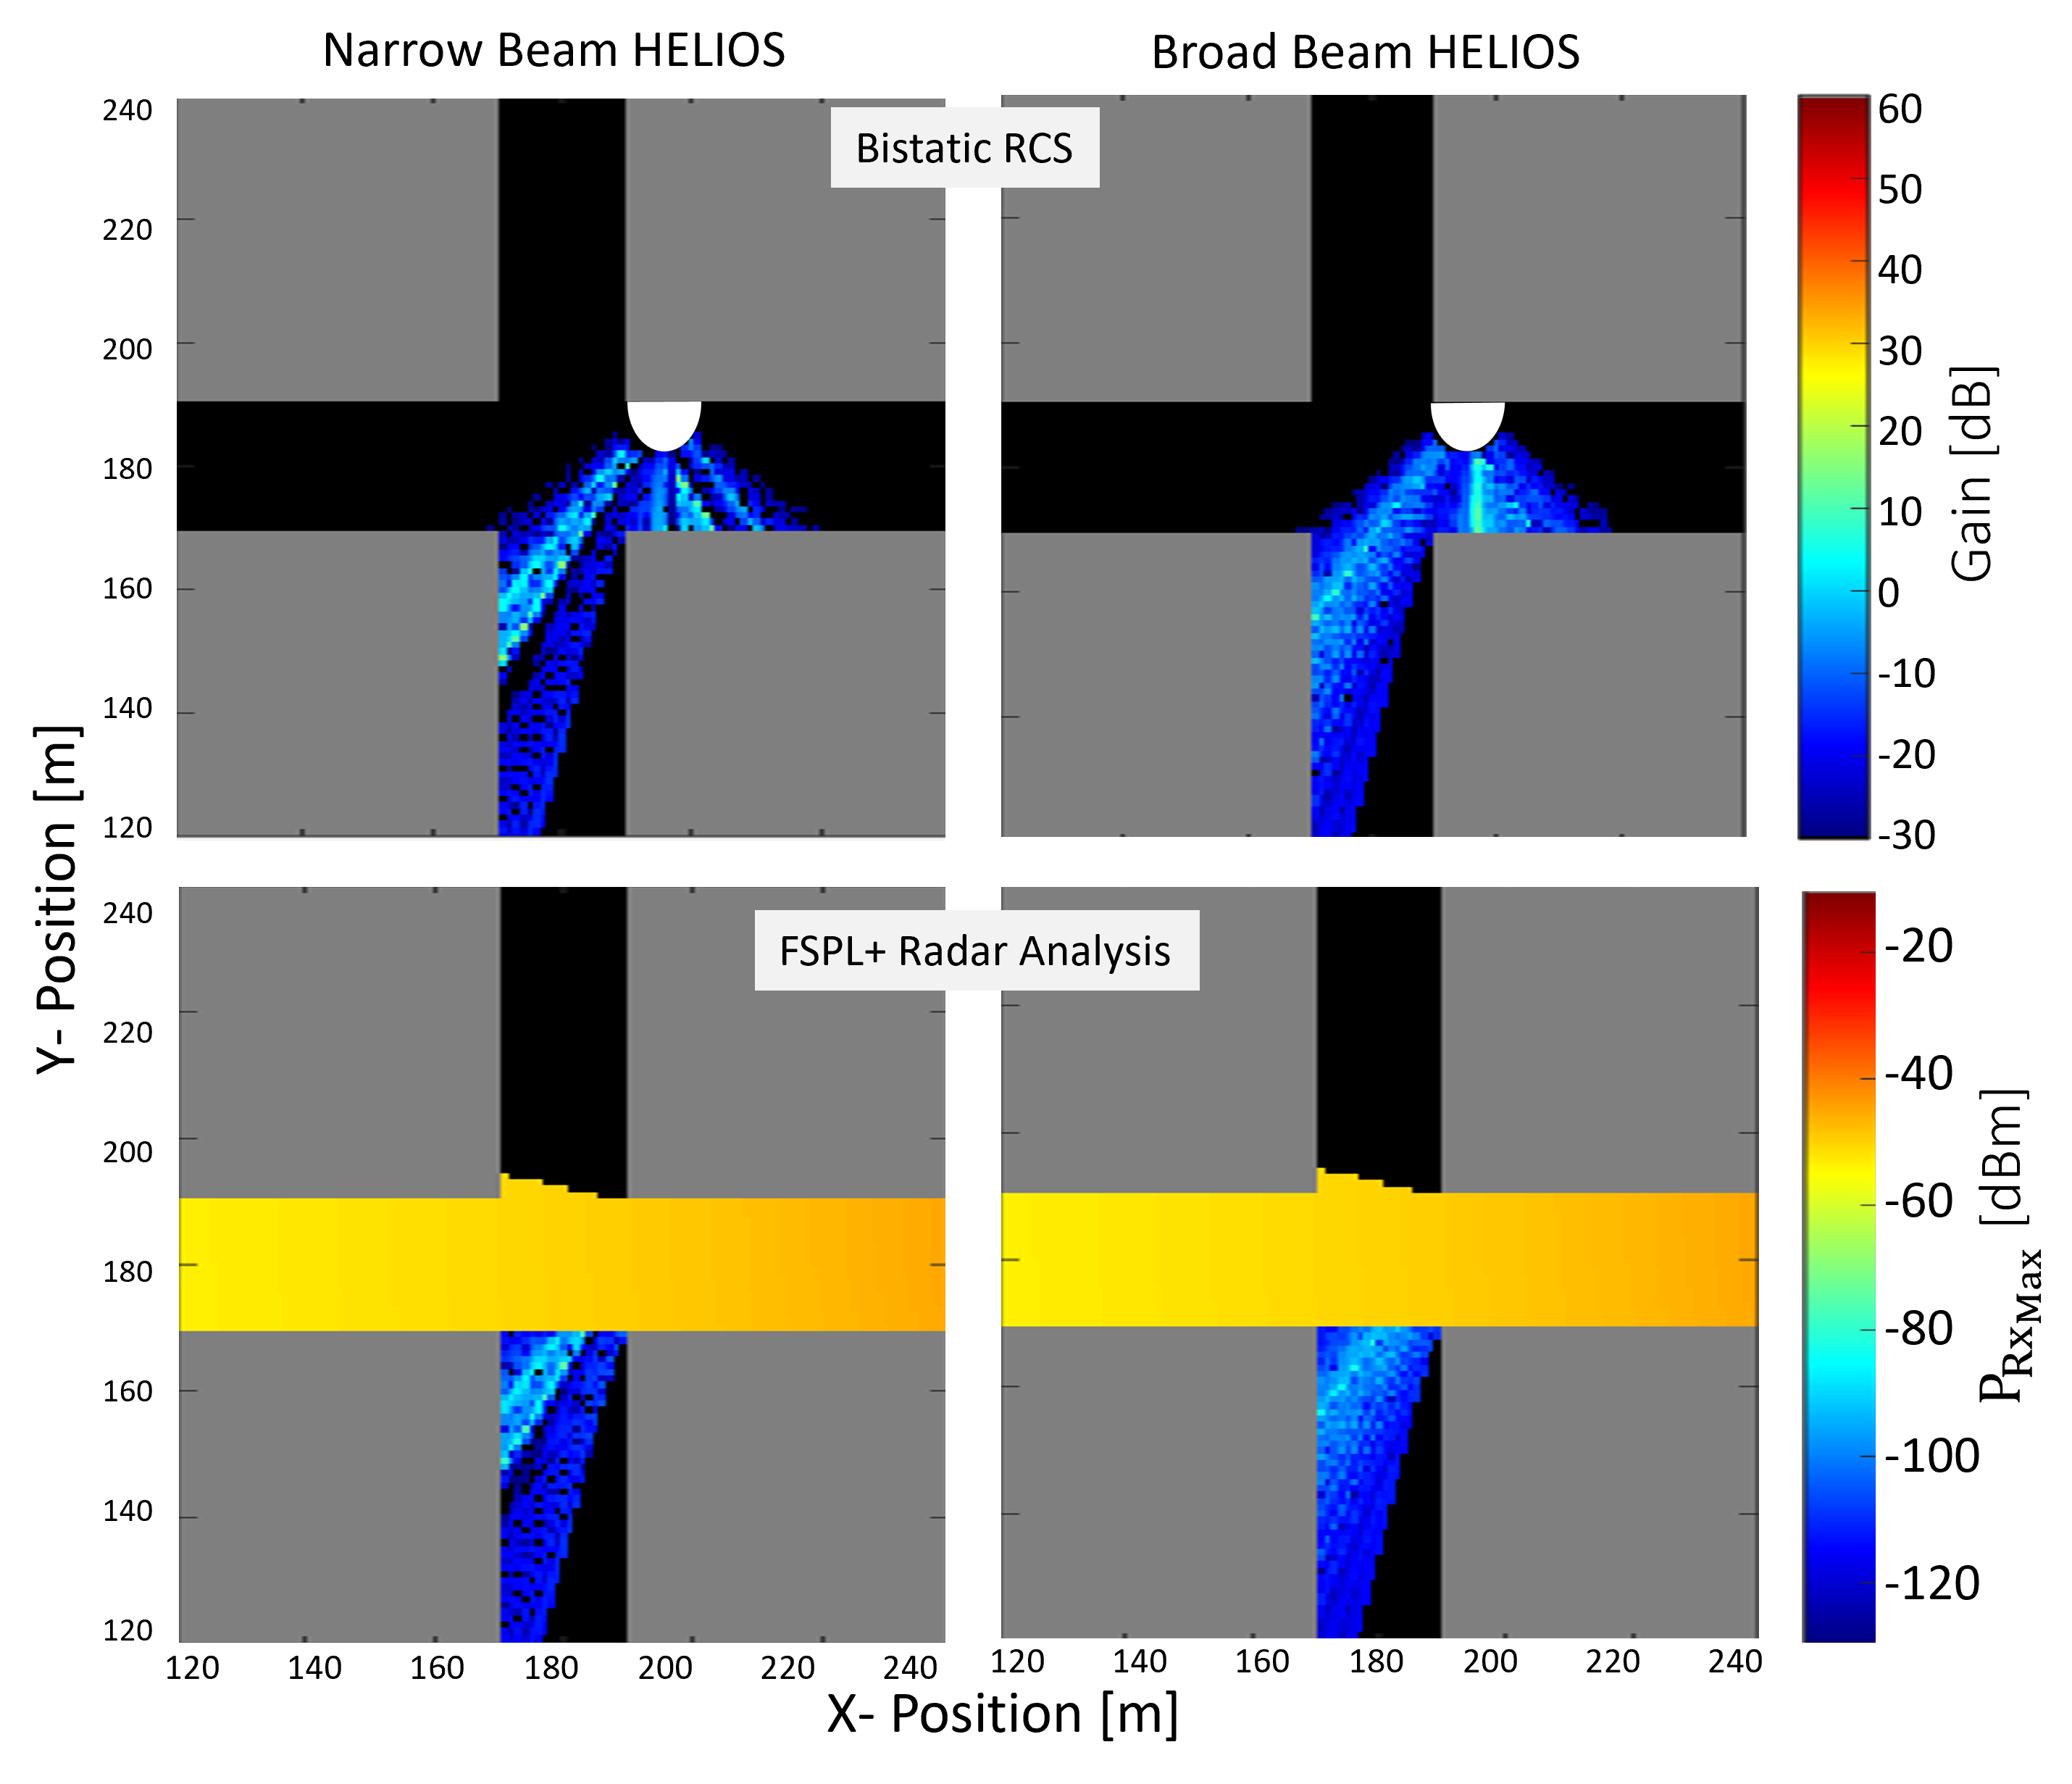
\includegraphics[width=0.8\linewidth]{images/Section 4 Images/urbanscenario_originalvalues}
	\caption{RCS comparison of narrow beam HELIOS (left column) and broad beams HELIOS (right column) in an urban scenario depicting the gain in \si{\decibel} (top row) and maximum power received in \si{\decibel}m (bottom row). The parameters are considered from \Cref{Table:Urban case study} at \SI{28}{\giga\hertz} frequency. Notably, the power is radiating in the direction of south street canyon with a peak gain of \SI{15.4}{\decibel} with narrow beam and \SI{11.2}{\decibel} with broad beam. }
	\label{fig:urbanscenario_originalvalues}
\end{figure}
Even if the LOS zones appear to be unaffected, \Cref{fig:Scenario2} confirms that the reflector, which has a minimum power $>$ \SI{-83.5}{\decibel}m, introduces unique propagation characteristics in the LOS region. Observing the behavior in the south street canyon, there is a significant difference in coverage regions between narrow and broad beams HELIOS. The heatmap's visual depiction of signal coverage fluctuations shows how tight beams have concentrated, localized effects while broad beam HELIOS has a broader range of influence. This finding highlights the tactical benefit of using a HELIOS configuration aiming for a broader distribution of the reflection. However, the overall coverage in south street canyon is noted to be around \num{1}\% with both narrow and broad beam HELIOS. A closer look at the RCS heatmaps at the bottom shows where the maximum power received is distributed. They are mainly in the LOS region and not in the region of interest, thus motivating a revision of the HELIOS configurations being considered in the next sections. 
\subsection{Optimizing Connectivity by Improving upon HELIOS Geometry}\label{Optimizing the HELIOS Geometry for Better Performance}
We used previously determined slope angle values from the literature \cite{Helios} in our earlier analysis. Now, we use our analytical model systematically to identify a suitable HELIOS configuration so that our connectivity goals are met. Whereas such an optimization topic is out of the scope of this work, we show here how our analytical model can be put to use there due to the short computing times, see \Cref{Computing Time Analysis}. We note that this would not be possible in such short time when using EM simulations. We investigated widely for slope angles $\alpha_{m,n}$, and $\beta_{m,n}$ to accomplish this optimization. With a $\num{0.2}^\circ$ step size, the slope angle ranges from $\alpha_{m,n} \in [15: 35]^\circ$ and $\beta_{m,n} \in [-10: 10]^\circ$. Overall, more than $10,000$ RCS pattern calculations were used to identify a more suitable HELIOS narrow beam and broad beam configuration, respectively.

It is important to remember that for narrow beams, the slope angle values for each of the \num{32} reflector parts stay constant, whereas, on the other hand, the slope angles must differ for broad beams. As such, there are two degrees of freedom to optimize the narrow beam HELIOS reflector configuration, i.e., $\alpha=\alpha_1 = \dots = \alpha_{32}$ and $\beta=\beta_1 = \dots = \beta_{32}$. For the revision of the broad beam HELIOS, we configure these variables precisely in our reflector design process. Our approach necessitates that each of the \num{32} modules have its slope angles carefully assigned inside the reflector design. With a step increment of $\num{2.5}^\circ$ between each angle for both the slope angles, each module is specifically assigned one of seven different slope angles. This complex operation is as complex as described in the literature \cite{Helios}, and adjusting this step value has not been shown to result in meaningful improvements.\\
The RCS heatmap depicting our search for a narrow beam HELIOS inside our chosen region of interest is shown in \Cref{fig:urbanscenario_narrowsearch}. Here, each pixel in the heatmap is already the sum of the received power of the given HELIOS configuration. Finding the peak power received location, which acts as our reference point, is our main goal. We find the matching slope angles $\alpha_{m,n}$ and $\beta_{m,n}$ by locating the maximum value inside the heatmap. For instance, as seen by a little black box inside the image in \Cref{fig:urbanscenario_narrowsearch}, the maximum value happens at $\alpha=\num{30.2}^\circ$ and $\beta=\num{4.2}^\circ$. 
\begin{figure}[H]
	\centering
	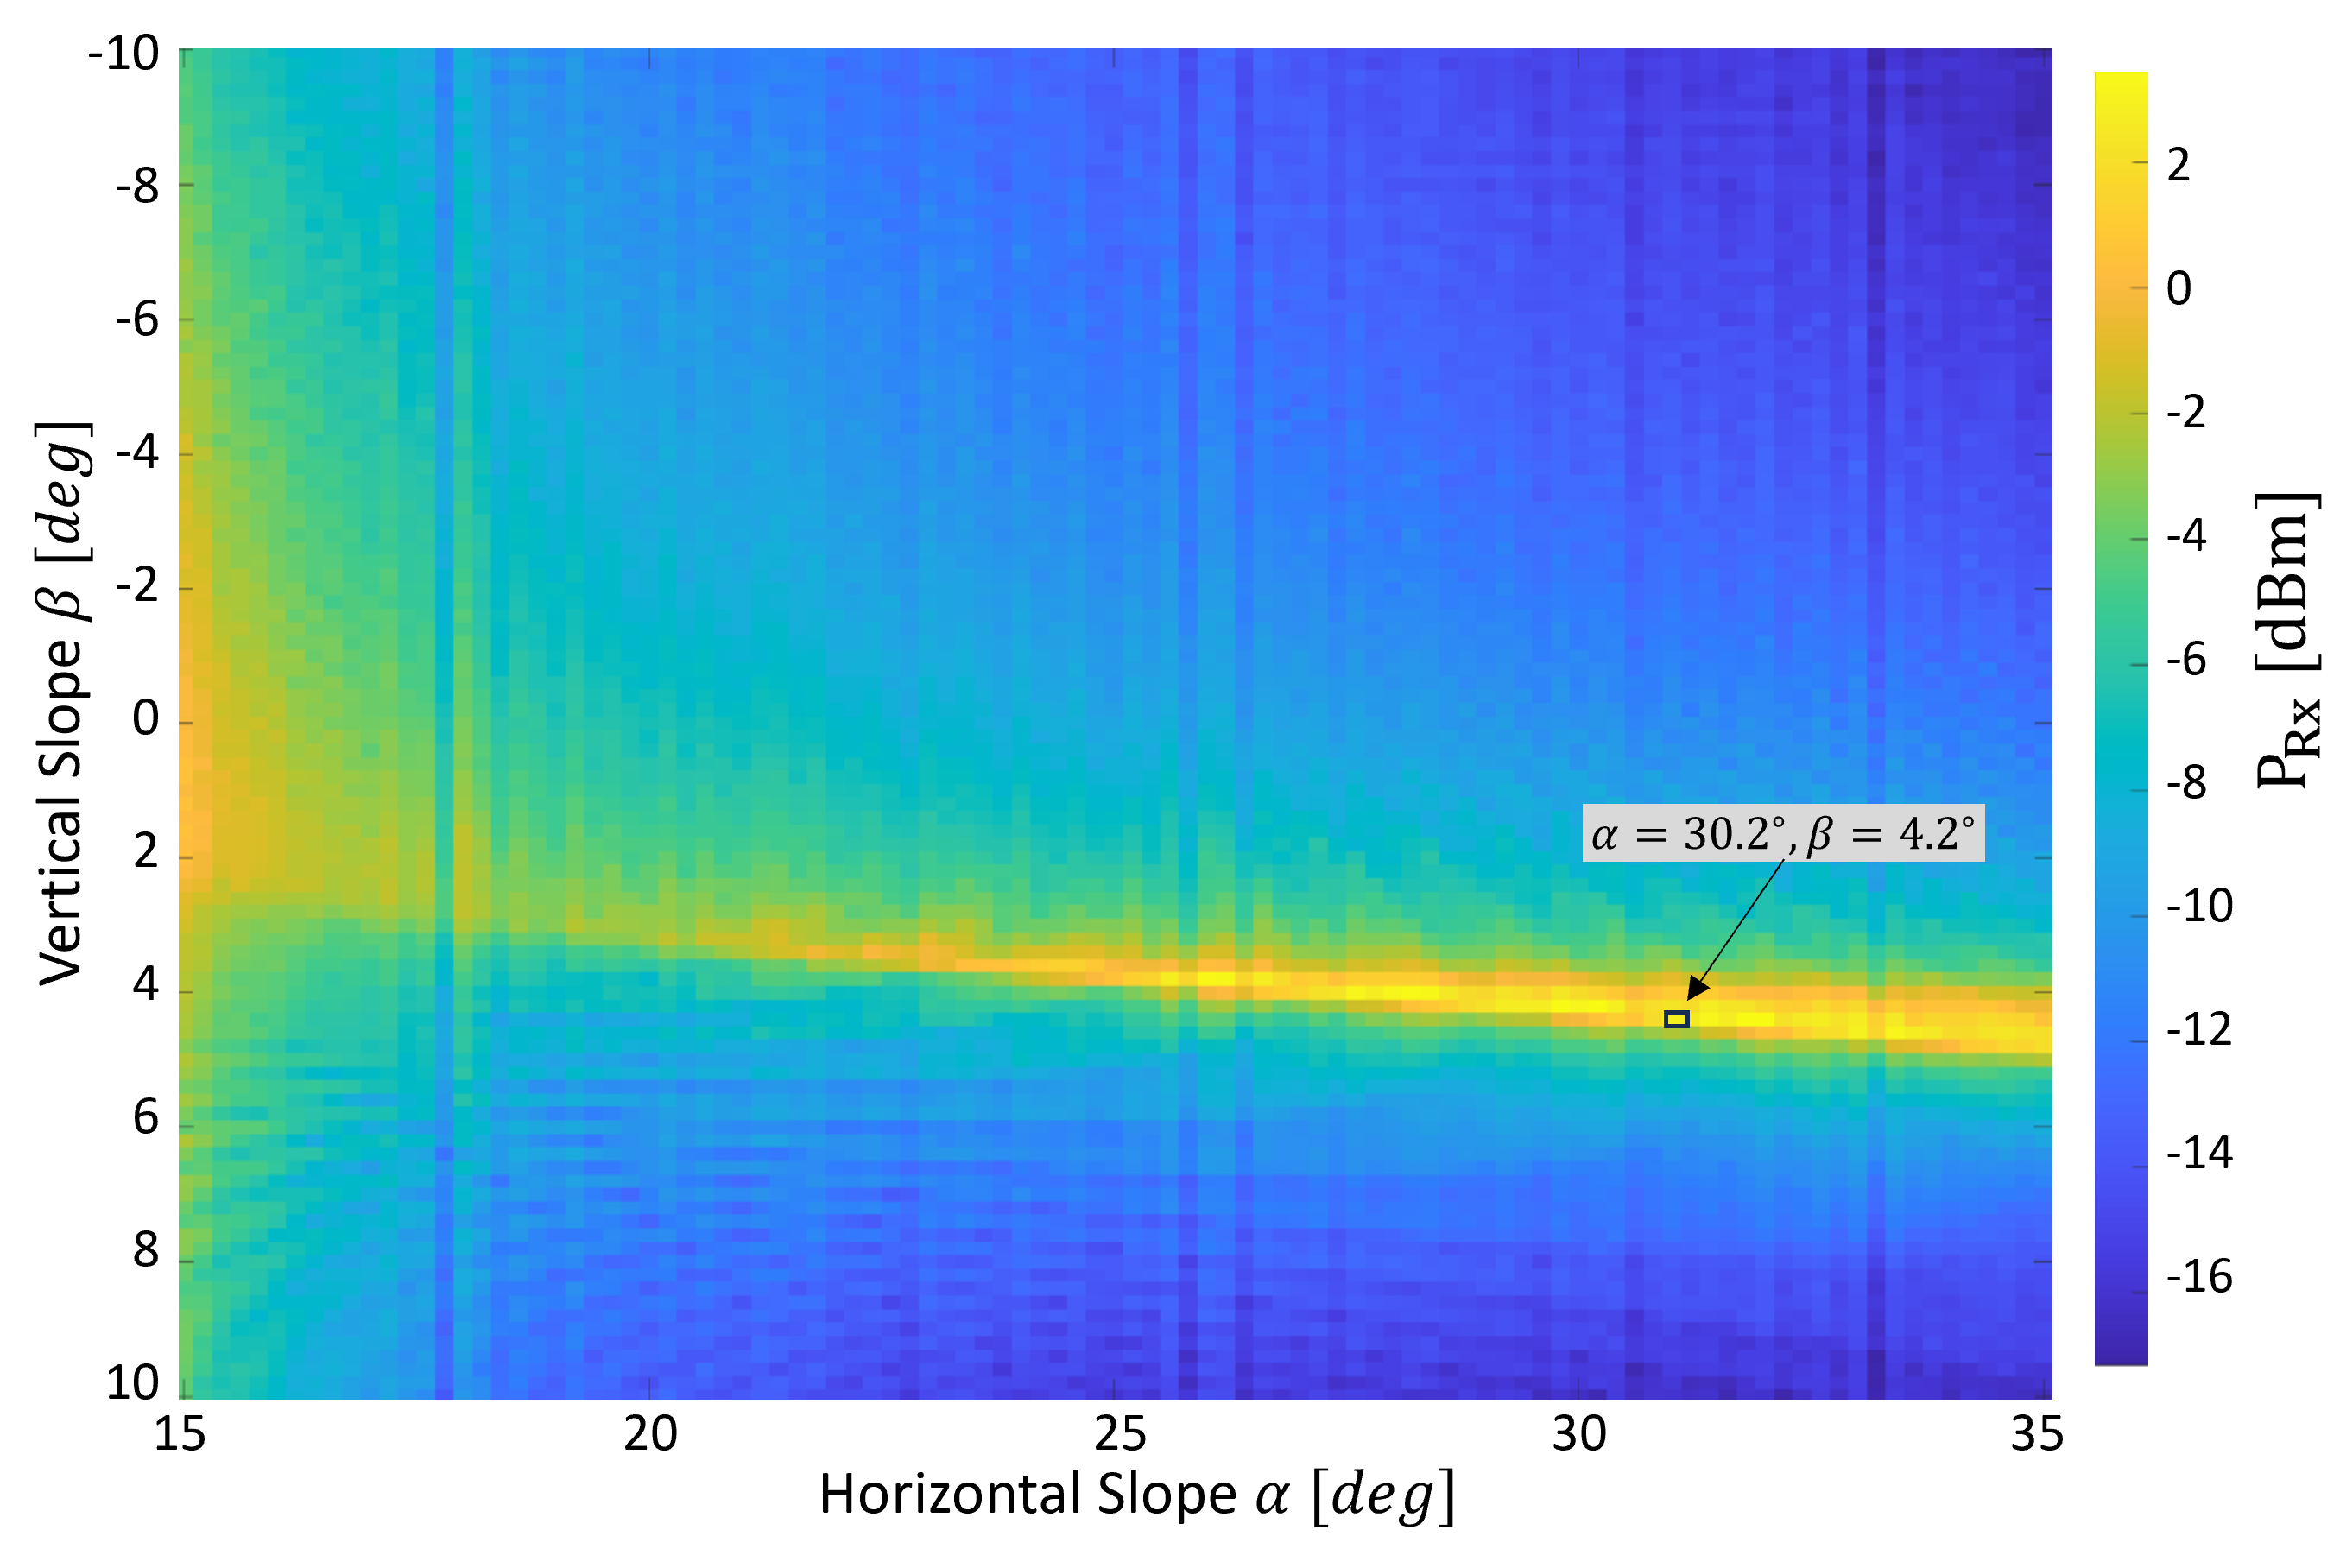
\includegraphics[width=0.78\linewidth]{images/Section 4 Images/urbanscenario_narrowsearch}
	\caption{Power received RCS heatmap depicting the search for optimal slope angles to form narrow beams in the south street canyon of the urban scenario, resulting in the maximum power received at slope angle $\alpha=\num{30.2}^\circ$ and $\beta=\num{4.2}^\circ$, as depicted by the small black box.}
	\label{fig:urbanscenario_narrowsearch}
\end{figure}
Similarly, \Cref{fig:urbanscenario_broadsearch} provides the search heatmap for broad beam HELIOS, where the maximum receive power is with slope angles $\alpha_{1,1}=\num{20.2}^\circ$ and $\beta_{1,1}=\num{-10.2}^\circ$. 
\begin{figure}[H]
	\centering
	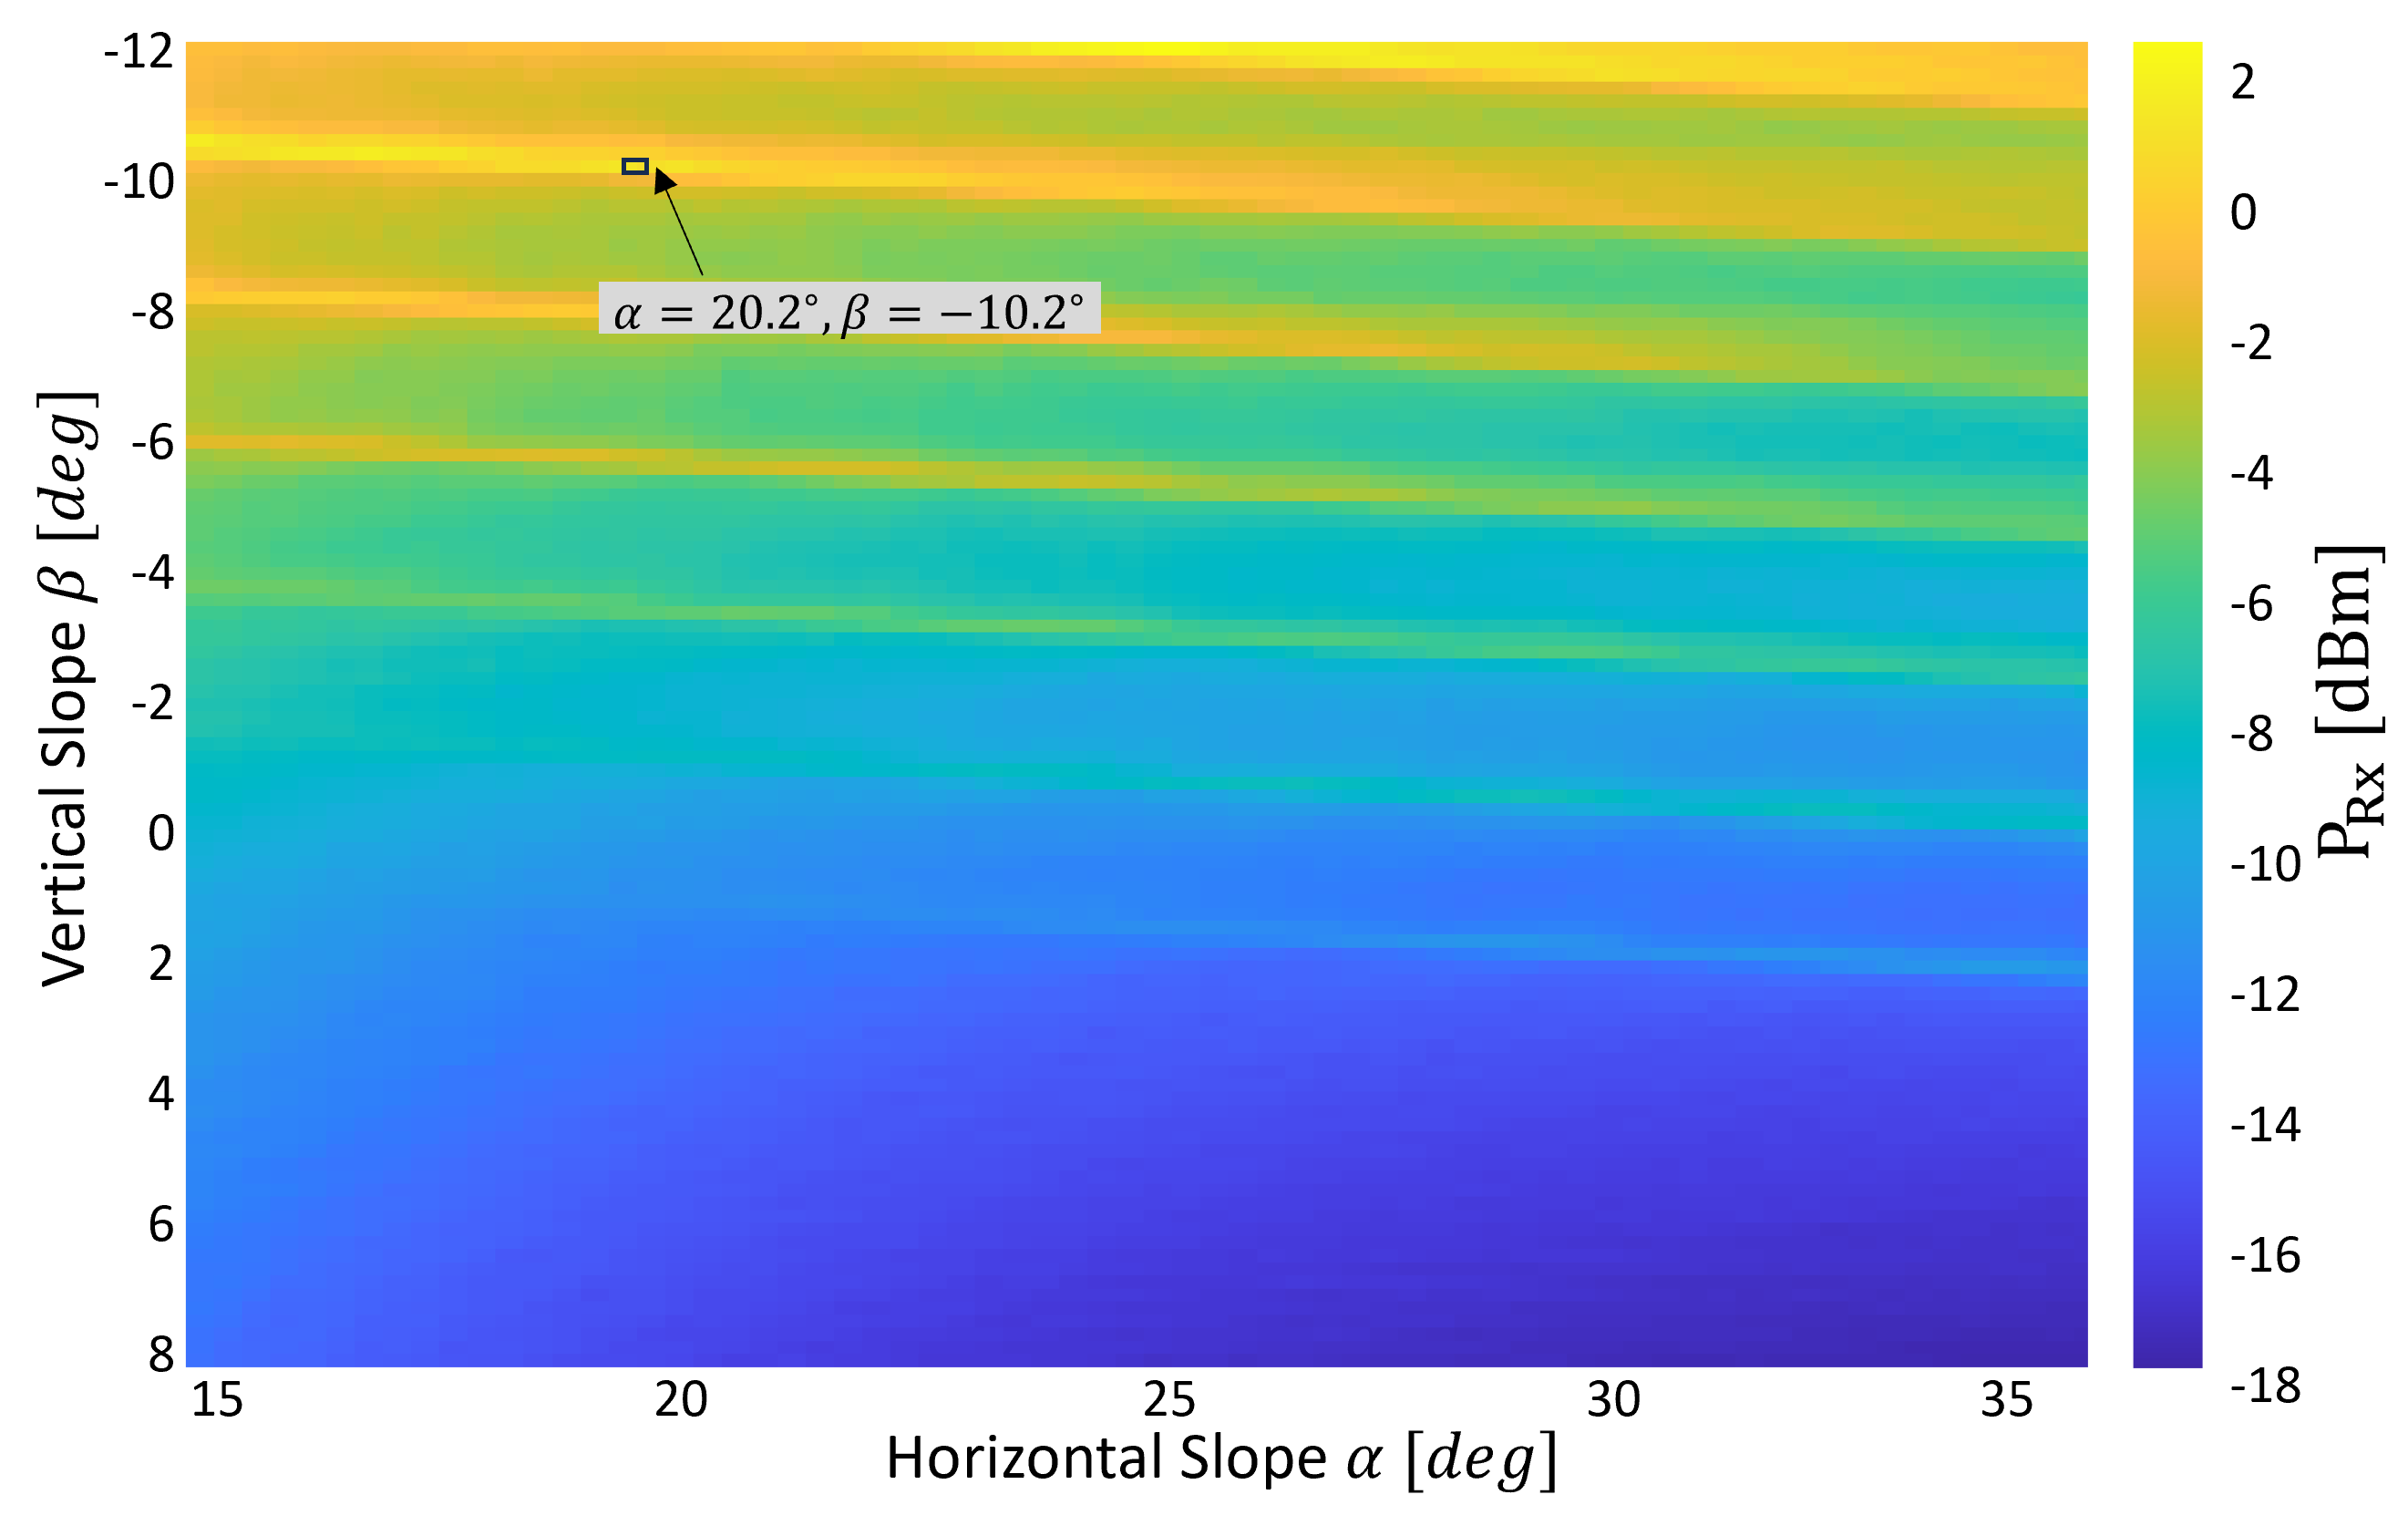
\includegraphics[width=0.78\linewidth]{images/Section 4 Images/urbanscenario_broadsearch}
	\caption{RCS received power depicting the search for optimal slope angles to form a broad beam in the south street canyon of the urban scenario. The \num{32} reflectors take seven different slope angles in the step of $\num{2.5}^\circ$ with $\alpha=\num{20.2}^\circ$ and $\beta=\num{-10.2}^\circ$ being its first value, where the maximum receive power is at this location. }
	\label{fig:urbanscenario_broadsearch}
\end{figure}
The reflectors then take seven different slope angles in the step of $\num{2.5}^\circ$ as depicted in \Cref{Urban Scenario Implementation}. Summarizing the above two paragraphs, we have identified the following optimized HELIOS configurations:
\begin{itemize}
	\item \textbf{Optimized narrow beam HELIOS}: Slope angle $\alpha_{1}=...=\alpha_{32}=\num{30.2}^\circ$, and $\beta_{1}=...=\beta_{32}=\num{4.2}^\circ$.
	\item \textbf{Optimized broad beam HELIOS}: Slope angle variation in the steps of $\num{2.5}^\circ$, $\alpha_{1},....,\alpha_{32} \in [\num{20.2}:\num{35.2}]^\circ$, i.e., $\alpha_{2}, \alpha_{1}= \num{20.2}^\circ$, $\alpha_{6}, ...., \alpha_{3}=  \num{22.7}^\circ$, $\alpha_{11}, ...., \alpha_{7}= \num{25.2}^\circ$, $\alpha_{17}, ...., \alpha_{12}= \num{27.7}^\circ$, $\alpha_{23}, ...., \alpha_{18}= \num{30.2}^\circ$, $\alpha_{28}, ...., \alpha_{24}= \num{32.7}^\circ$, and $\alpha_{32}, ...., \alpha_{29}= \num{35.2}^\circ$,
	and \\
	 $\beta_{1},....,\beta_{32} \in [\num{-10.2}:\num{4.8}]^\circ$, $\beta_{2}, \beta_{1}= \num{-10.2}^\circ$, $\beta_{6}, ...., \beta_{3}=  \num{-7.7}^\circ$, $\beta_{11}, ...., \beta_{7}= \num{-5.2}^\circ$, $\beta_{17}, ...., \beta_{12}$ $=\num{-2.7}^\circ$, $\beta_{23}, ...., \beta_{18}= \num{-0.2}^\circ$, $\beta_{28}, ...., \beta_{24}= \num{2.3}^\circ$, and $\beta_{32}, ...., \beta_{29}= \num{4.8}^\circ$. 
\end{itemize}
Compared to the previous configuration, the adoption of the elevation slope parameter is an important aspect of our optimization process. In \Cref{Coupling Simulated and Analytical Reflection Pattern with Radar Realization}, we have considered the case when $\beta_{m,n}=0^\circ$, similar to that mentioned in \cite{Helios}. However, given these intrinsic differences, comparing the optimized model to the earlier model is a little unfair. 
\begin{figure}[H]
	\centering
	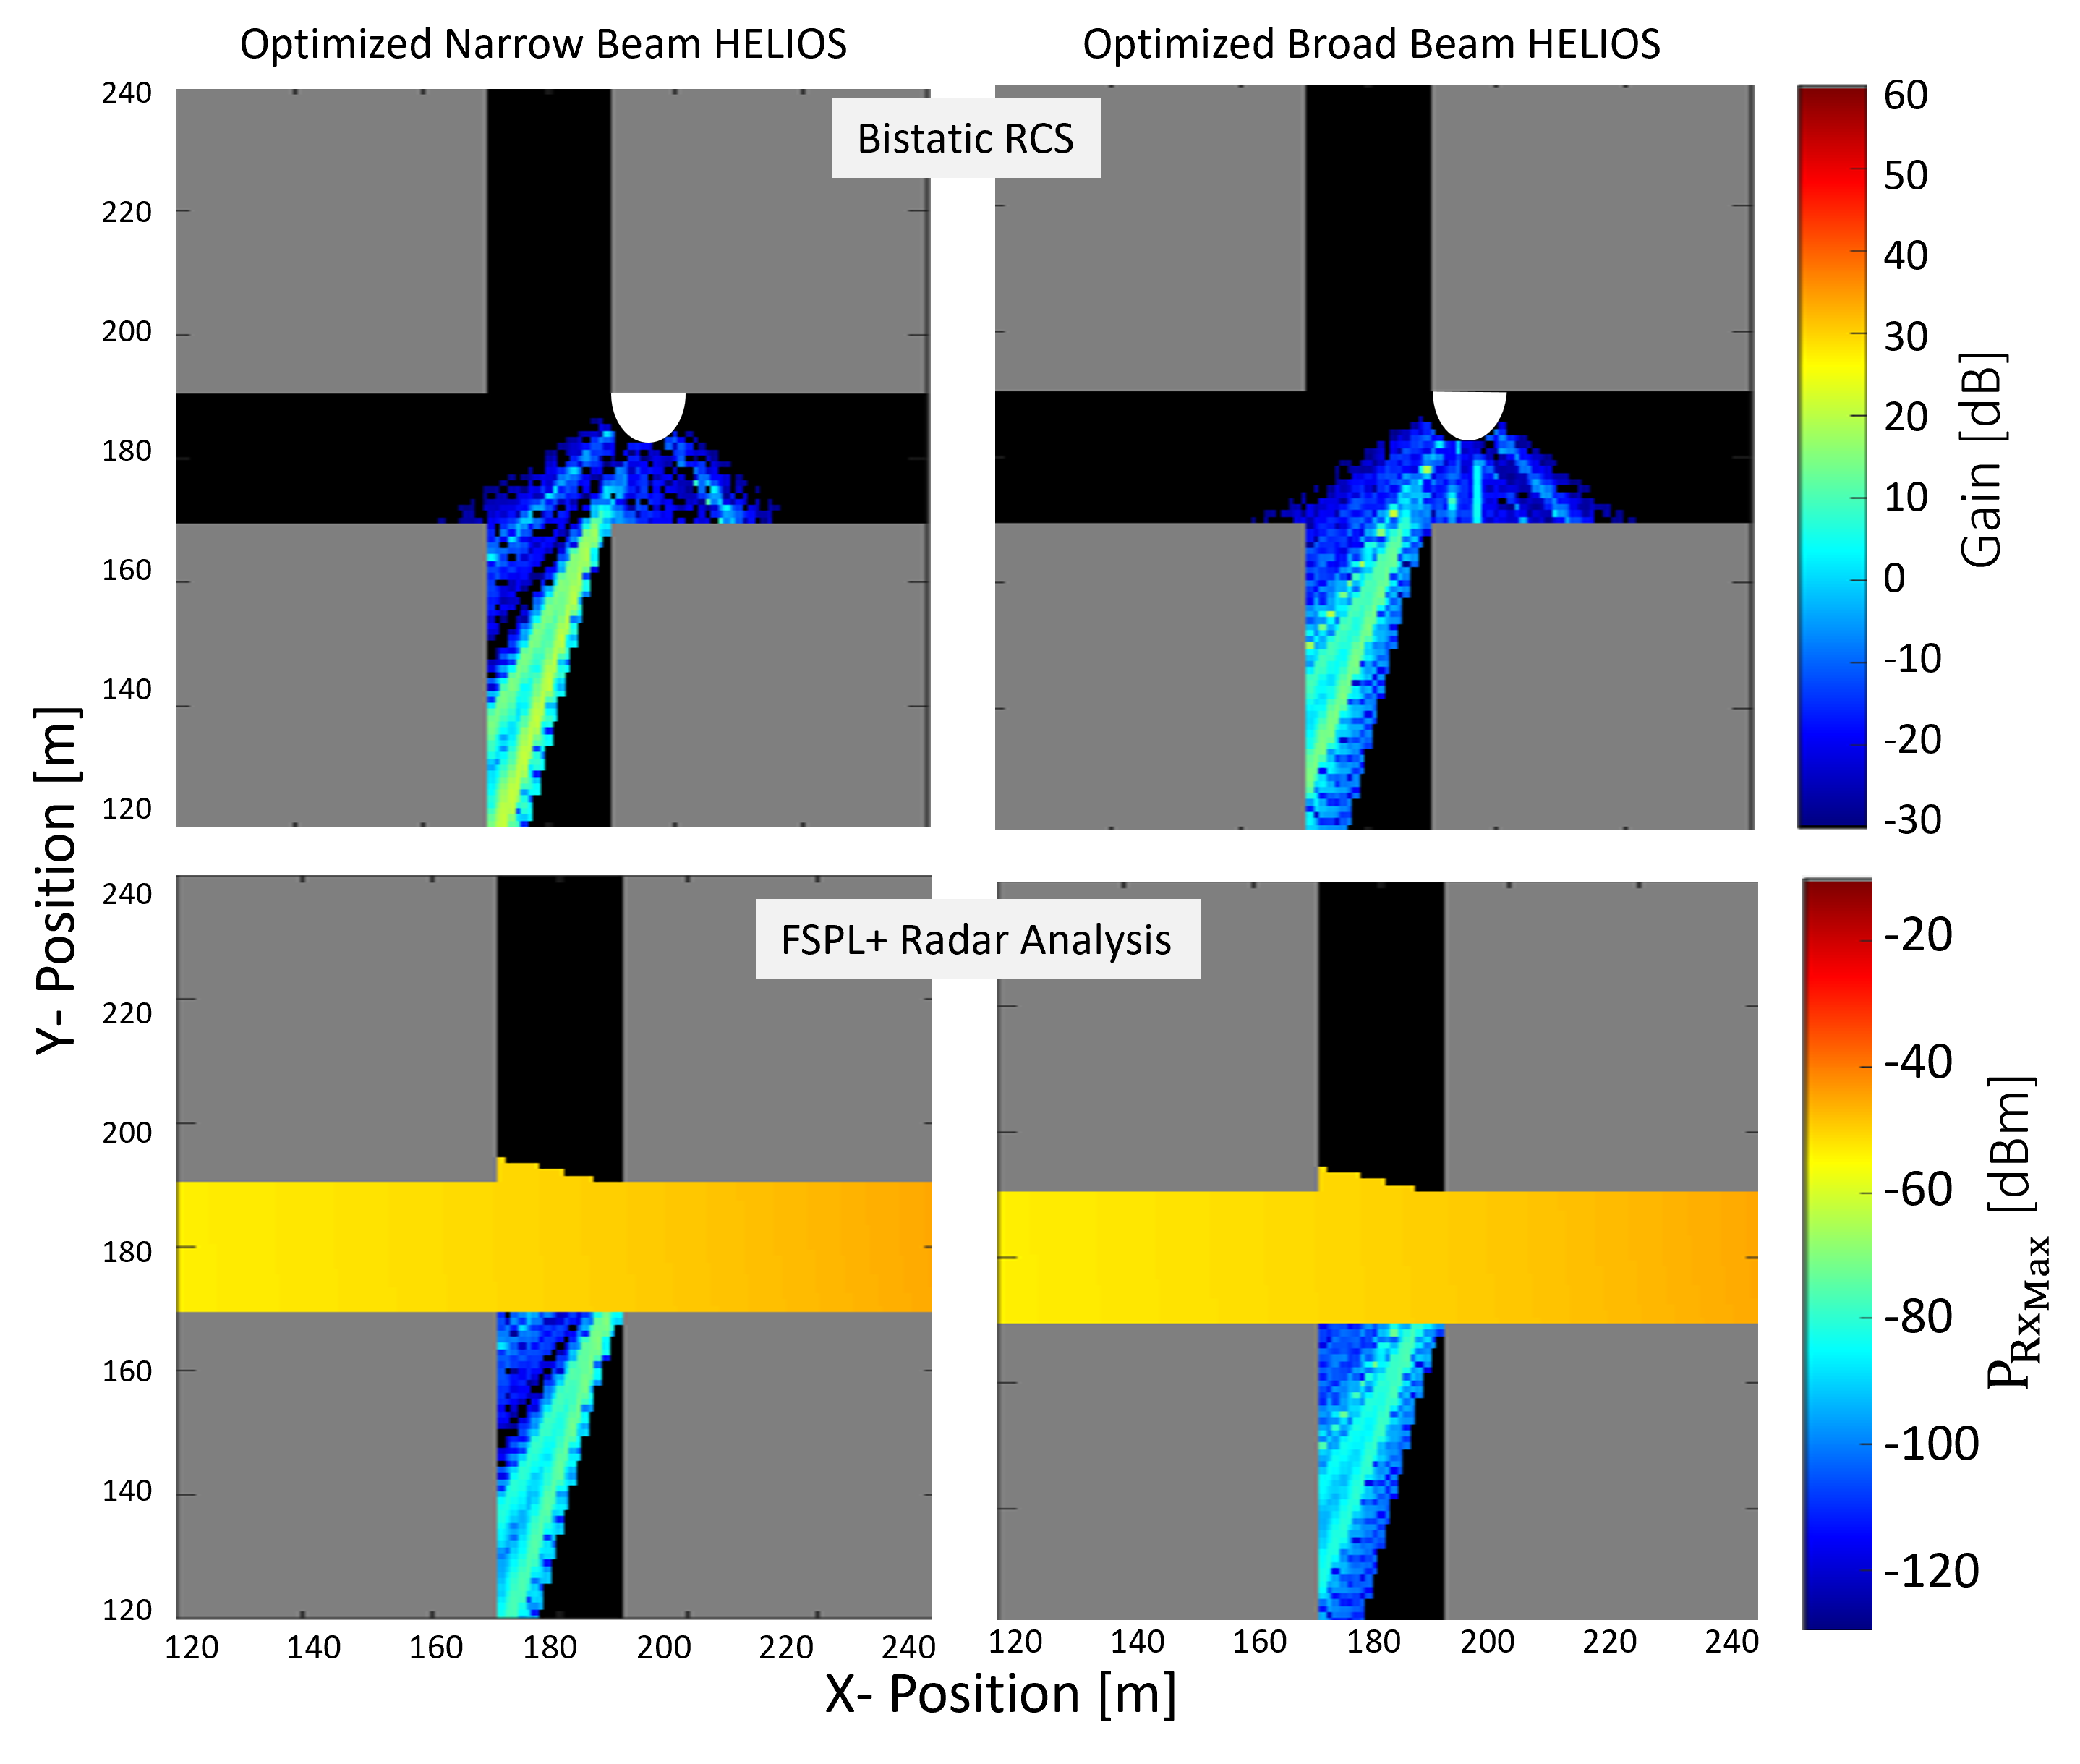
\includegraphics[width=0.8\linewidth]{images/Section 4 Images/urbanscenario_optimzedvalues}
	\caption{RCS comparison of narrow beam HELIOS (left column) and broad beams HELIOS (right column) in an urban scenario depicting the gain in \si{\decibel} (top row) and maximum power received in \si{\decibel}m (bottom row). The parameters are considered from \Cref{Table:Urban case study} at \SI{28}{\giga\hertz} frequency with the optimized slope angles.}
	\label{fig:urbanscenario_optimzedvalues}
\end{figure}
Interestingly, we correct this imbalance in our methodology by utilizing recently unexplored aspects to strengthen the strength of the assessment, a tactical advantage not found in earlier methods. Analog to \Cref{fig:urbanscenario_originalvalues} in \Cref{Coupling Simulated and Analytical Reflection Pattern with Radar Realization}, we assess the expected performance in our street crossing scenario in \Cref{fig:urbanscenario_optimzedvalues}. The maximum power received is displayed in the bottom row of the picture, while the top row depicts the gain behavior of the reflectors. When compared to \Cref{fig:urbanscenario_originalvalues}, considerable improvements have been made by this optimization approach. The improved slope angles result in a maximum gain of \SI{20.5}{\decibel} for narrow beams ($+\SI{5.1}{\decibel}$) and \SI{19.9}{\decibel} for broad beams ($+\SI{8.7}{\decibel}$).

Our optimized slope angles have even more advantages, as seen by the comparison with  \Cref{fig:urbanscenario_optimzedvalues}. In addition to being more comprehensive, the coverage inside our chosen region of interest performs better, i.e., approx. \num{8.3}\% with narrow beam HELIOS and around \num{15.0} \% with broad beam HELIOS. Our approach is thus effective in optimizing slope angles for both narrow and broad beams in the urban context, as demonstrated by the improved gain and power reception capabilities. In the given urban context, this improvement has proven to be crucial in obtaining enhanced signal strength and communication.
\subsection{Optimizing Connectivity for Different Reflector Position}\label{Optimizing Connectivity with Different Reflector Positions}
Our previous results, e.g., \Cref{fig:urbanscenario_optimzedvalues}, indicate that a fraction of the region of interest is still not covered. This is due to the reflector position. Thus, we now move the reflector \SI{3.5}{\meter} to the west, i.e., right to the building edge, and rerun the optimization process from \Cref{Optimizing the HELIOS Geometry for Better Performance}. Thereby, we illustrate how the analytical model could be used during hybrid network planning. The optimization process yields the following configurations:
\begin{itemize}
	\item \textbf{Optimized narrow beam HELIOS: Edge}: Slope angle $\alpha_{1}=...=\alpha_{32}=\num{10.4}^\circ$, and $\beta_{1}=...=\beta_{32}=\num{2.2}^\circ$.
	\item \textbf{Optimized broad beam HELIOS: Edge}: Slope angle variation in the steps of $\num{2.5}^\circ$, 	$\alpha_{1},....,\alpha_{32} \in [\num{-6.5}:\num{8.5}]^\circ$, i.e., $\alpha_{2}, \alpha_{1}= \num{-6.5}^\circ$, $\alpha_{6}, ...., \alpha_{3}=  \num{-4}^\circ$, $\alpha_{11}, ...., \alpha_{7}= \num{-1.5}^\circ$, $\alpha_{17}, ...., \alpha_{12}= \num{1}^\circ$, $\alpha_{23}, ...., \alpha_{18}= \num{3.5}^\circ$, $\alpha_{28}, ...., \alpha_{24}= \num{6}^\circ$, and $\alpha_{32}, ...., \alpha_{29}= \num{8.5}^\circ$,
	and \\
	$\beta_{1},....,\beta_{32} \in [\num{-4.6}:\num{10.4}]^\circ$, i.e., $\beta_{2}, \beta_{1}= \num{-4.6}^\circ$, $\beta_{6}, ...., \beta_{3}=  \num{-2.1}^\circ$, $\beta_{11}, ...., \beta_{7}= \num{0.4}^\circ$, $\beta_{17}, ...., \beta_{12}= \num{2.9}^\circ$, $\beta_{23}, ...., \beta_{18}= \num{5.4}^\circ$, $\beta_{28}, ...., \beta_{24}= \num{7.9}^\circ$, and $\beta_{32}, ...., \beta_{29}= \num{10.4}^\circ$. 
\end{itemize}
Similar to our analysis in \Cref{Optimizing the HELIOS Geometry for Better Performance}, we consider RCS and received power heatmaps along the scenario using the two newly optimized HELIOS configurations at the new mounting positions. \Cref{fig:urbanscenario_edgevalues}'s top row shows the gain behavior, while the bottom row shows the maximum power, i.e., also considering LOS contributions, that were received. When comparing to \Cref{fig:urbanscenario_optimzedvalues}, one can extract from \Cref{fig:urbanscenario_edgevalues} that the change of mounting of position and thereafter rerunning of the optimization algorithm is fruitful: In particular, maximum gains of \SI{29.1}{\decibel} for narrow beams and \SI{38.9}{\decibel} for broad beams are attained, constituting increases of \SI{8.6}{\decibel} and \SI{19}{\decibel}, respectively. These results highlight how important reflection beamwidth is in affecting the system's overall performance.

\begin{figure}[tb]
	\centering
	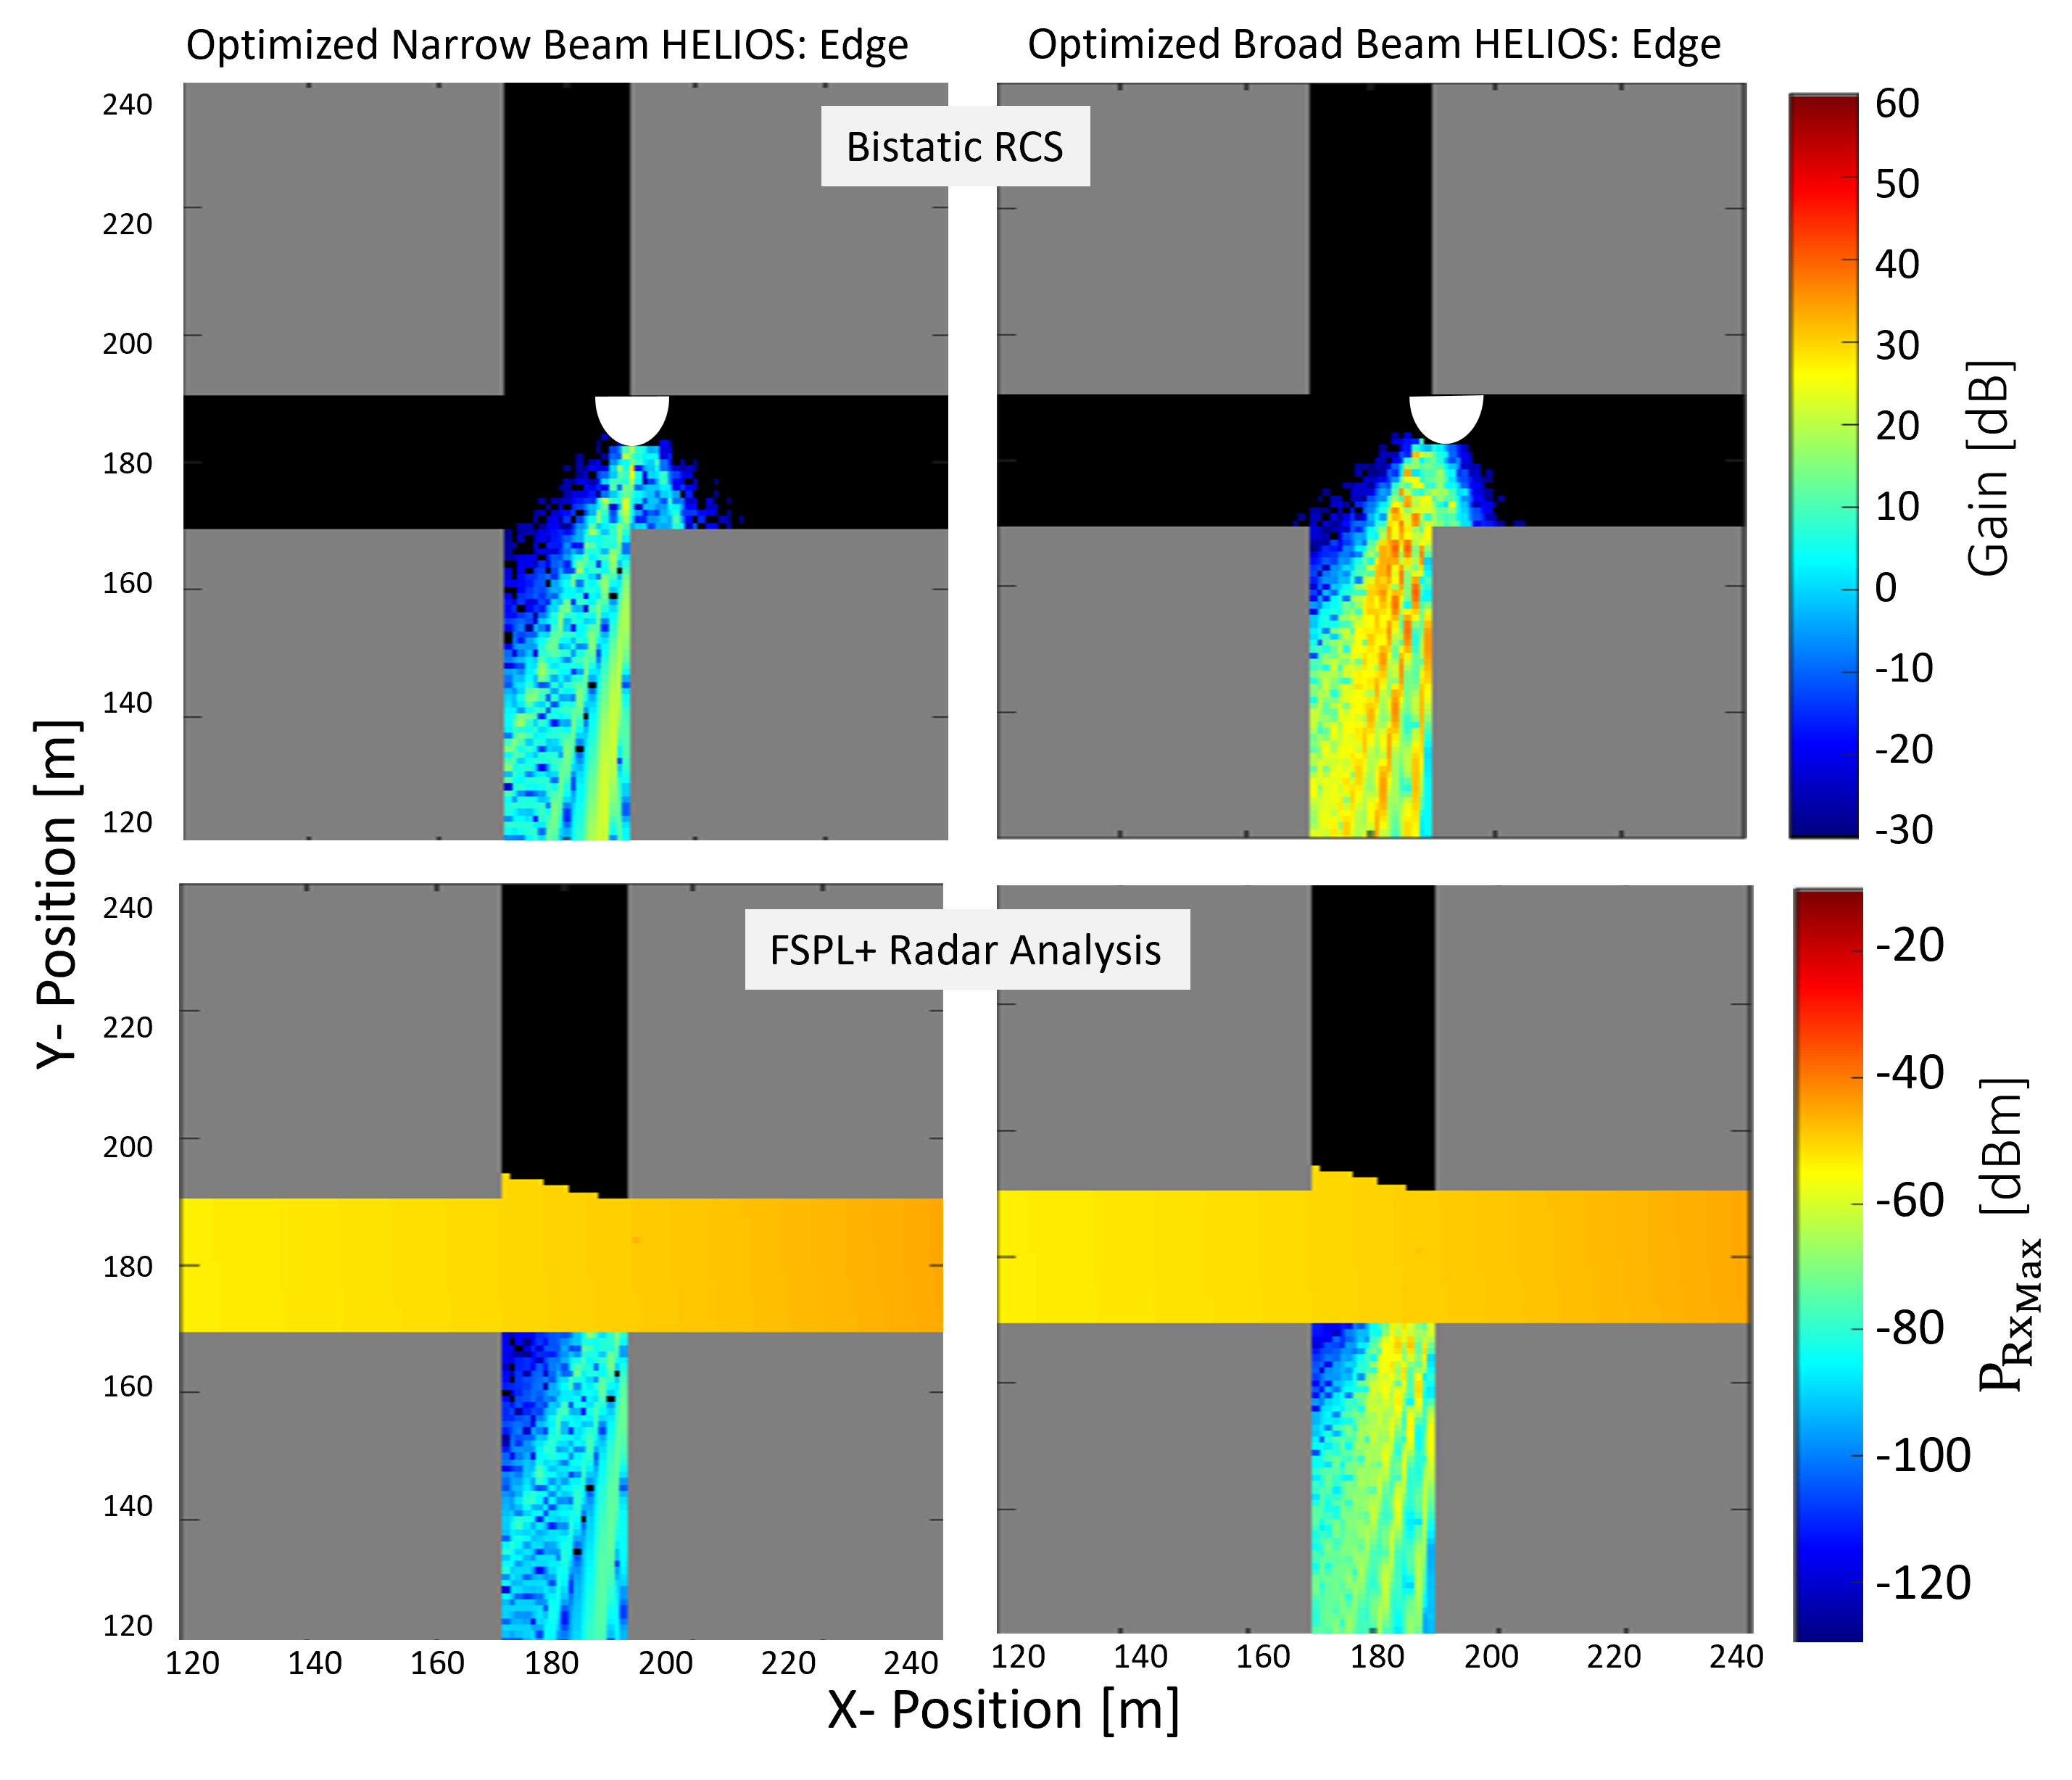
\includegraphics[width=0.8\linewidth]{images/Section 4 Images/urbanscenario_edgevalues}
	\caption{RCS comparison of optimized narrow beam HELIOS (left column) and broad beams HELIOS (right column) in an urban scenario depicting the gain in \si{\decibel} (top row) and maximum power received in \si{\decibel}m (bottom row). The parameters are considered from \Cref{Table:Urban case study} at \SI{28}{\giga\hertz} frequency with the optimized slope angles at the edge of the building.}
	\label{fig:urbanscenario_edgevalues}
\end{figure}
Moreover, we can see that the adjusted reflector placement greatly improves both the coverage and performance within our region of interest. These constitute to coverage area of about \num{30.1} \% with narrow beam HELIOS and \num{79.3} \% with broad beam HELIOS. This coverage is better than the previous models in \Cref{fig:urbanscenario_optimzedvalues} and \Cref{fig:urbanscenario_originalvalues}.

To conclude, we have thereby shown the potential gains HELIOS reflectors may provide in such a scenario. In this context, we have shown the benefits a thorough optimization in terms of geometry configuration and mounting position may have. However, one must note that our attained performance does not constitute the global maxima. Future work on this optimization topic, which is out of the scope of this thesis, is likely to achieve even better results. 
\subsection{Analyzing IRS Based Connectivity}\label{Analyzing Urban Scenario for Different IRS Models}
Now that we have explored the performance of the analytical model for reflectors in urban scenarios, we may now compare the performance of HELIOS reflectors against IRSs using the respective analytical models from \Cref{coordinate systems}. Like in \Cref{Optimizing Connectivity with Different Reflector Positions}, the IRS shall be mounted at the more suitable, changed mounting position at the edge of the building to maximize the coverage in the south street canyon. This section considers two cases: First, we use the IRS model by Özdogan \emph{et al}. \cite{8936989} \Cref{Model 1} and consider it for a fixed configuration reflecting the energy in a bundle fashion into the region of interest. Second, we employ all three models \cite{8936989, ntontin2021optimal, tang2020wireless} and consider the maximum gain throughout the scenario for the case that the IRS is set to beamform to each possible UE position, thus contrasting the previous case.

Similar to our analysis from \Cref{fig:urbanscenario_narrowsearch}, the performance results with $\gamma_{Rx}(\theta_{Rx},\varphi_{Rx})=$ $\gamma_{Rx}$ $(\num{-2.5}^\circ$, $\num{-25.75}^\circ)$ yields the best to serve the south street canyon. The gain and power received RCS heatmaps in \Cref{fig:urbanscenario_IRSmodel1s} compare two separate instances shown in this model. In the first scenario, the user is positioned at the angle at which the IRS is precisely pointing also referred to as a "dynamic beam", i.e., when $\gamma_{Rx} = \gamma_{Dev}$. When $\gamma_{Rx} \neq \gamma_{Dev}$, i.e., a user-performed angle sweep is indicated in the second scenario which is also referred to as a "fixed beam". The latter scenario in this case leads to the narrow beams being generated.
\begin{figure}[H]
	\centering
	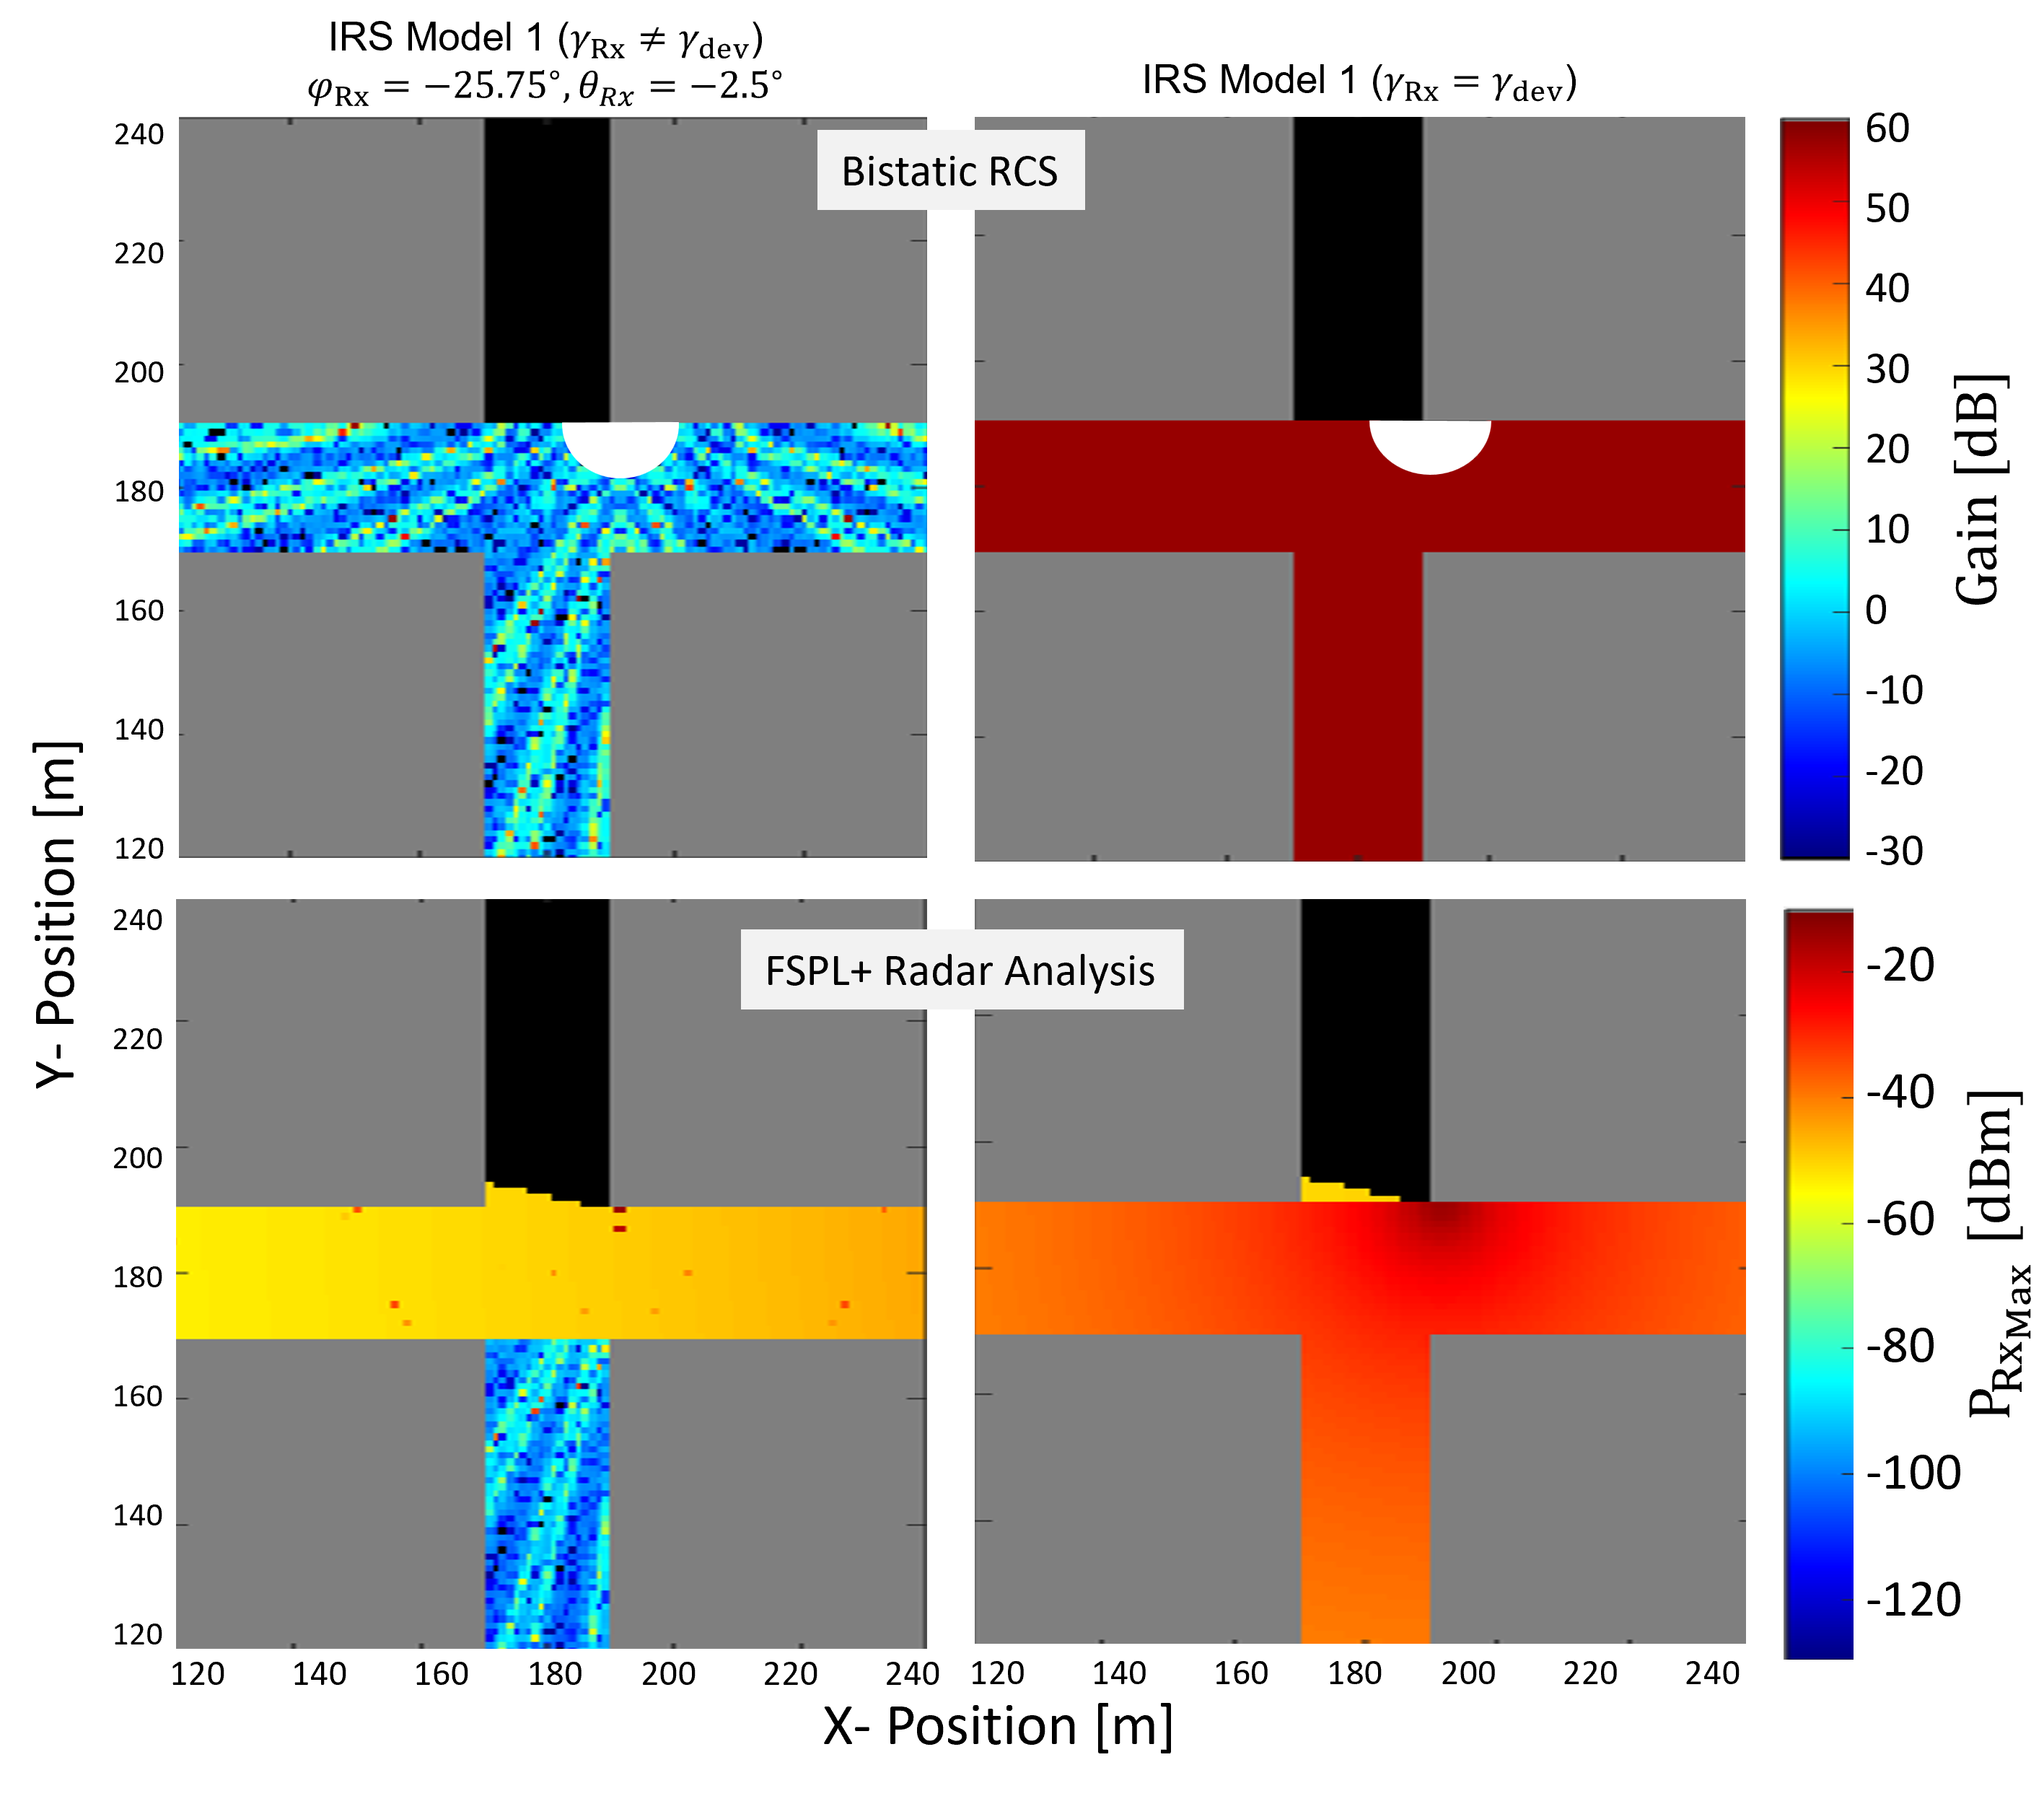
\includegraphics[width=0.8\linewidth]{images/Section 4 Images/urbanscenario_IRSmodel1s}
	\caption{RCS comparison of two cases of IRS model 1 (\Cref{Model 1}): fixed beam case on the left column and dynamic beam on the right column in an urban scenario depicting the gain in \si{\decibel} (top row) and maximum power received in \si{\decibel}m (bottom row). The parameters are considered from \Cref{Table:Urban case study} at \SI{28}{\giga\hertz} frequency with the optimized slope angles at the edge of the building.}
	\label{fig:urbanscenario_IRSmodel1s}
\end{figure}

The examination of maximum gain in \Cref{fig:urbanscenario_IRSmodel1s} shows that both fixed and dynamic beam cases of IRS model 1 have \SI{57.5}{\decibel} gain, which constitutes to increase by \SI{28.4}{\decibel} as compared to \Cref{fig:urbanscenario_edgevalues}. Comparison between RCS heatmaps by both the scenarios of model 1 is mainly in terms of beam pattern and coverage. The coverage area is almost \num{100} \% when $\gamma_{Rx}=\gamma_{Dev}$ (dynamic beam), whereas when the reflector focuses on the UE location (fixed beam), the coverage is \num{13.3} \%. This disparity highlights the multifaceted performance features of IRS model 1, in which the dynamic redistribution of signals occurs in different beam patterns and coverage areas while attaining the same advantages.

Turning our attention to \Cref{fig:urbanscenario_IRSmodel2_3}, which summarizes the results related to the other two IRS models discussed in \Cref{coordinate systems}. The peak gain for the second and third IRS models are \SI{57.5}{\decibel} and \SI{57.4}{\decibel}, respectively. These two models show coverage area in south street canyon by almost \num{97.7} \% and \num{100} \%, respectively, which are comparable to the results from the first IRS model with dynamic beam. The performance of IRS model 1 with the fixed beam is more comparable with our HELIOS analytical model in the urban scenarios with different reflector placement, see \Cref{Optimizing Connectivity with Different Reflector Positions}. A similar comparative analysis is carried out in \Cref{model gains}, but without the scenario implementation. 

\begin{figure}[H]
	\centering
	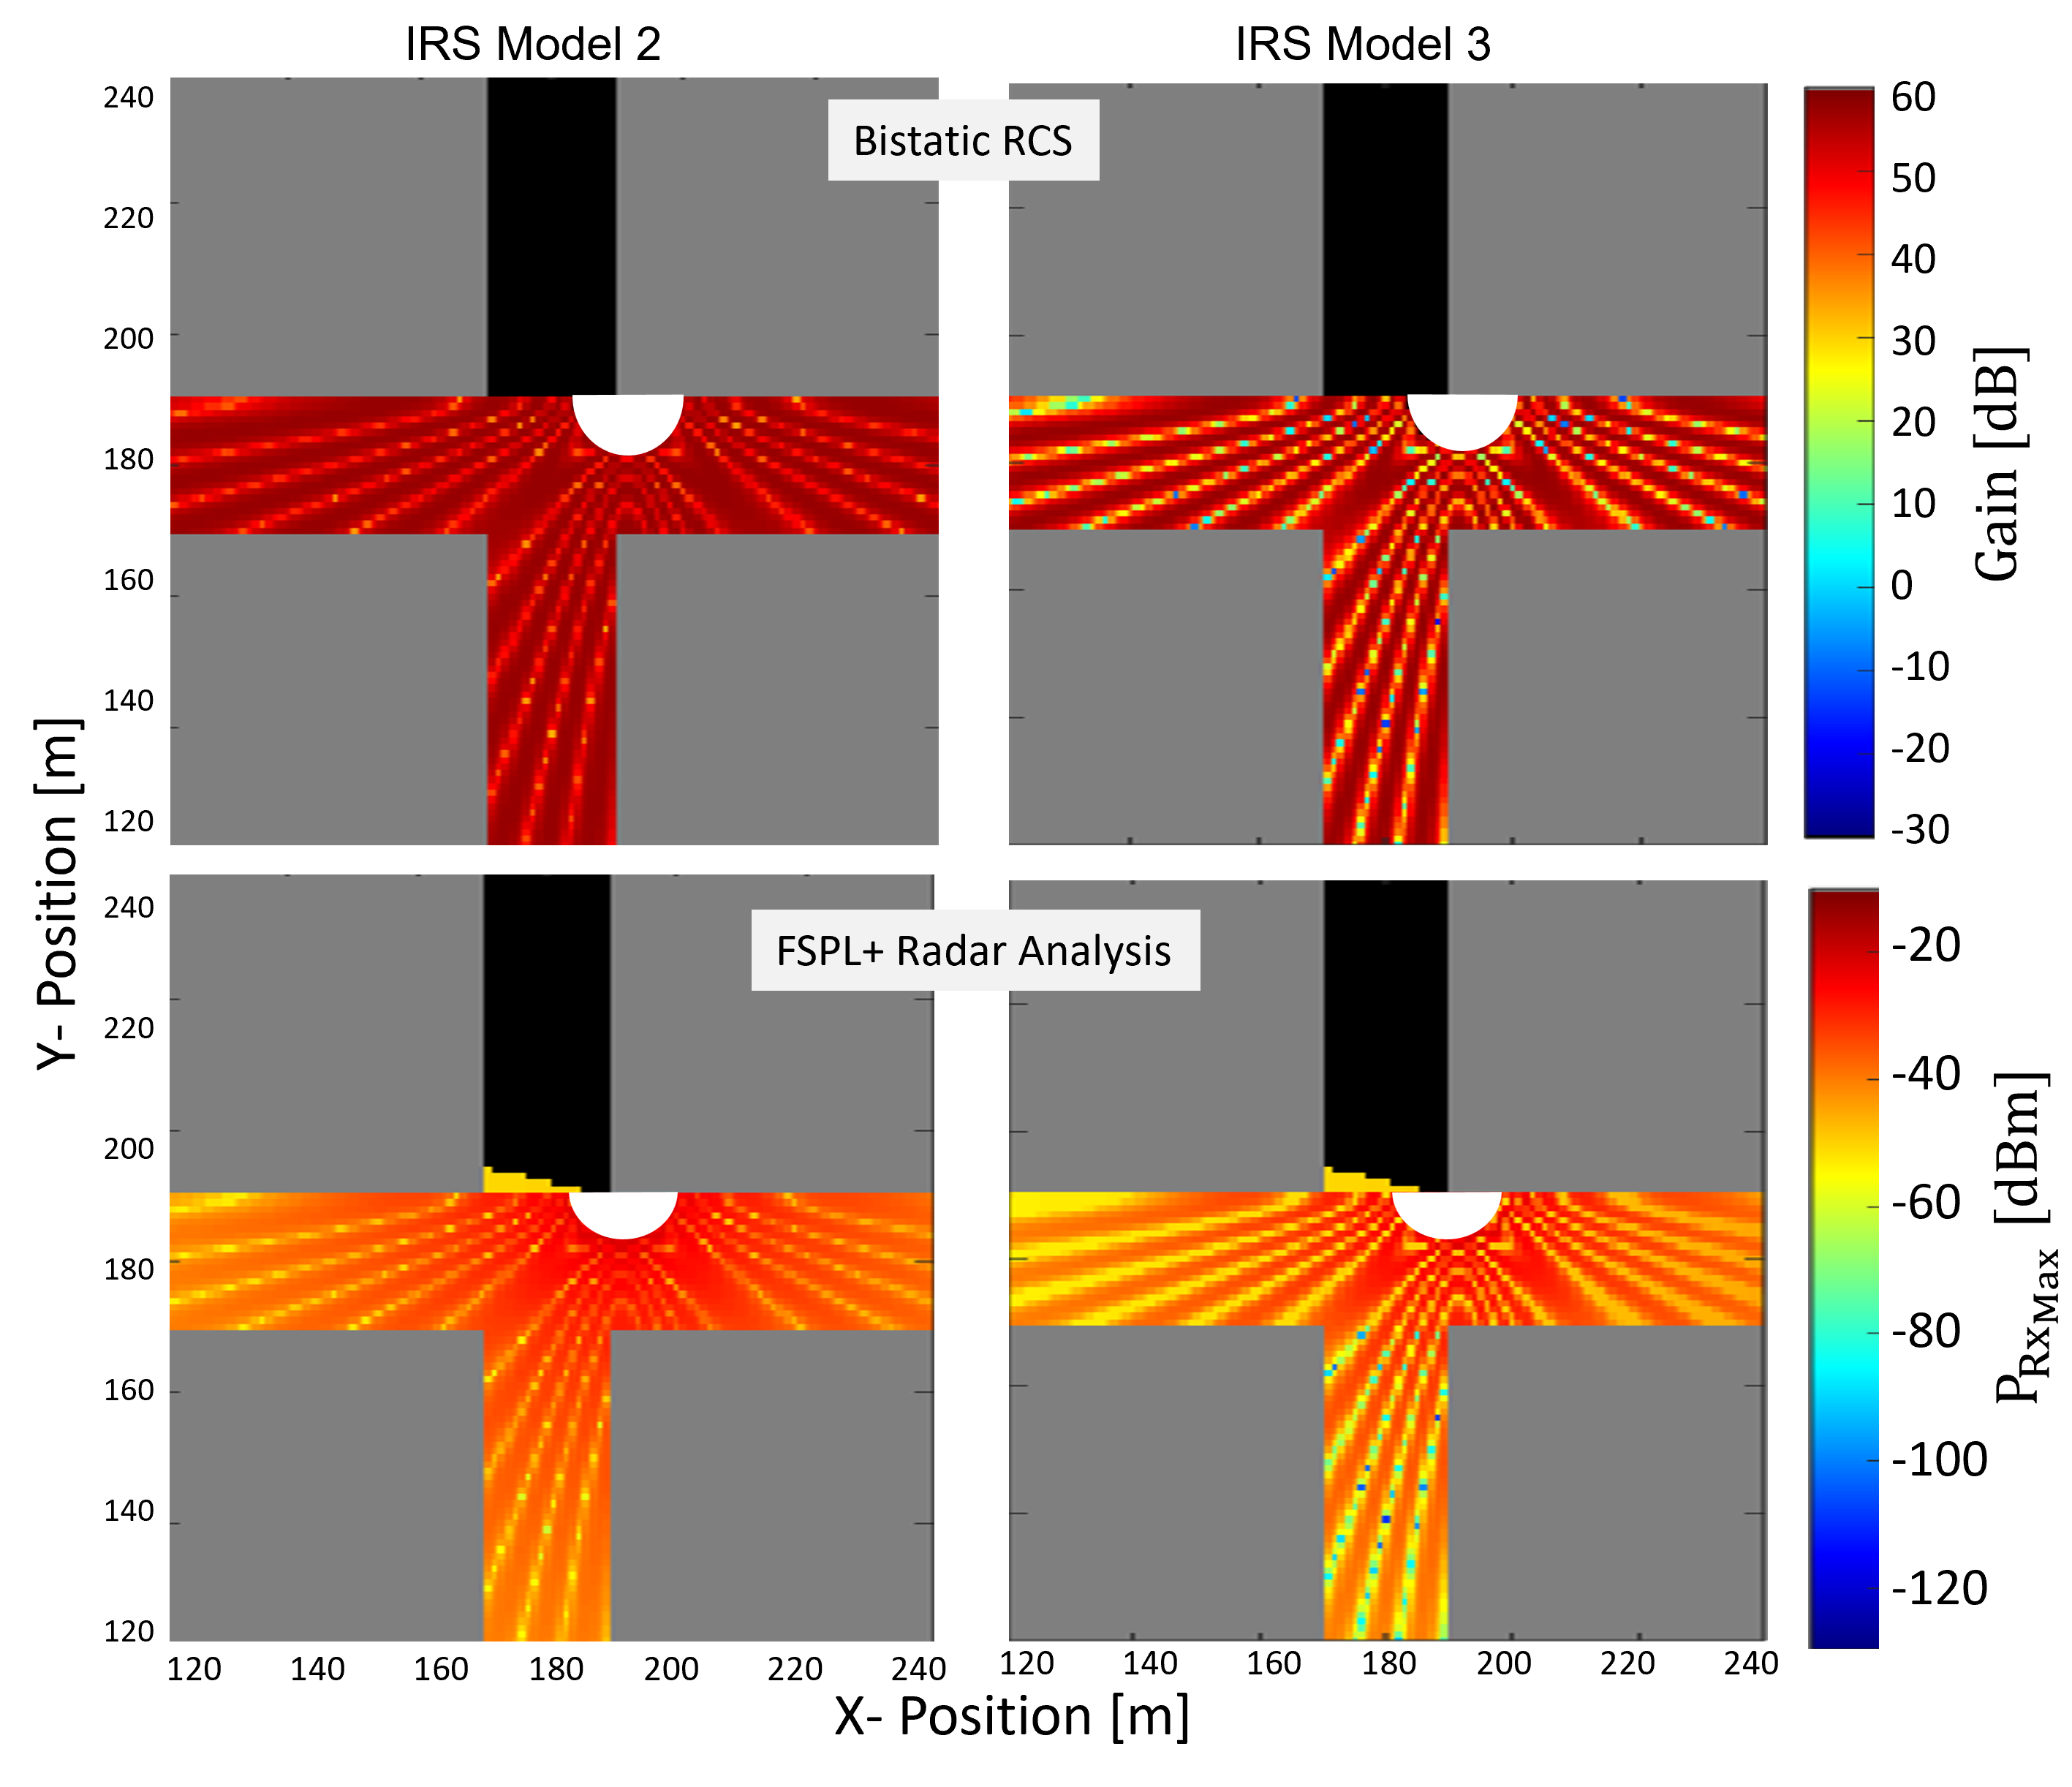
\includegraphics[width=0.8\linewidth]{images/Section 4 Images/urbanscenario_IRSmodel2_3}
	\caption{RCS comparison of IRS model 2 (left column) and IRS model 3 (right column) (\Cref{Model 3}) in an urban scenario depicting the gain in \si{\decibel} (top row) and maximum power received in \si{\decibel}m (bottom row). The parameters are considered from \Cref{Table:Urban case study} at \SI{28}{\giga\hertz} frequency with the optimized slope angles at the edge of the building.}
	\label{fig:urbanscenario_IRSmodel2_3}
\end{figure}

Further moving on to the detailed assessments of these models in \Cref{fig:urbanscenario_originalvalues}, \Cref{fig:urbanscenario_optimzedvalues}, \Cref{fig:urbanscenario_edgevalues}, \Cref{fig:urbanscenario_IRSmodel1s}, and \Cref{fig:urbanscenario_IRSmodel2_3} can be observed in \Cref{Comparing Passive Analytical Model to Active IRS Models}. The intrinsic ability of IRS models to effectively serve several locations and their dynamic signal redirection capabilities, which let them modify and improve the transmission path to accommodate various user locations, is what distinguishes them. These IRS models' adaptability and versatility highlight how important they are for improving signal propagation and increasing coverage in a variety of settings.
\subsection{Comparison of IRS and HELIOS based Connectivity Enhancements}\label{Comparing Passive Analytical Model to Active IRS Models}
We thoroughly investigated our HELIOS reflector performances in prior sections. This required a thorough examination of the baseline connectivity for a variety of channel models, which enabled us to make insightful comparisons with simulated outcomes from \cite{Helios}. We conducted a lengthy investigation to improve the reflectors' performance in our particular area of interest. This entailed carefully adjusting the reflectors' geometry and placement to maximize their effectiveness and match the special qualities of the region we had chosen. Moreover, our investigation went beyond a theoretical examination, as we used the IRS models in our urban scenario. We showed the strong connectivity such large IRSs could provide in the whole area when beamformed to the respective UE positions.

In this section, we now directly compare the three IRS models with the analytical HELIOS reflectors in great detail. The goal of this analysis is to draw attention to the advantages, and disadvantages of these two strategies. A detailed ECDF plot shown in \Cref{fig:Perfect_result_plot} illustrates the power received in \si{\decibel\meter} within the selected region of interest. \Cref{Baseline Performance of FSPL Model}, \Cref{Optimizing the HELIOS Geometry for Better Performance}, \Cref{Optimizing Connectivity with Different Reflector Positions}, and \Cref{Analyzing Urban Scenario for Different IRS Models} of this analysis provide a comparative examination of several reflector configurations. Our main goal is to clarify the differences in performance between different settings.

A significant finding is revealed when analyzing the reflector geometries covered in \Cref{Baseline Performance of FSPL Model}, and \Cref{Coupling Simulated and Analytical Reflection Pattern with Radar Realization}: The curves indicate that there is a potential coverage possible in the south street canyon region if the RCS directed to this area was higher. The changed HELIOS position shows that it is in a better mounting position for the intended south street coverage by \num{35}–\num{40} $\%$. The deliberate emplacement of reflectors, five meters from the building's edge, is responsible for this decrease, as they do not serve some part of the intended coverage region. when moving the reflector to a more suitable mounting position closer to the edge of the building, we observe a great impact as the whole region of interest is now in LOS from the reflector. HELIOS indeed enables mmWave connectivity in \num{80.2} \% of the area of interest, with mean and maximum receive powers of \SI{-75.2}{\decibel}m and \SI{-49.3}{\decibel}m. The behavioral analysis of IRS models is also included in \Cref{fig:Perfect_result_plot}. Compared to passive reflectors, the IRSs function better, offering better coverage and stronger signals. This superiority results from the IRS's dynamic nature, which allows them to focus on each UE position individually. The capacity of IRS to dynamically optimize signal propagation, surpassing conventional designs, makes them a clear advantage over passive reflectors.
\begin{figure}[H]
	\centering
	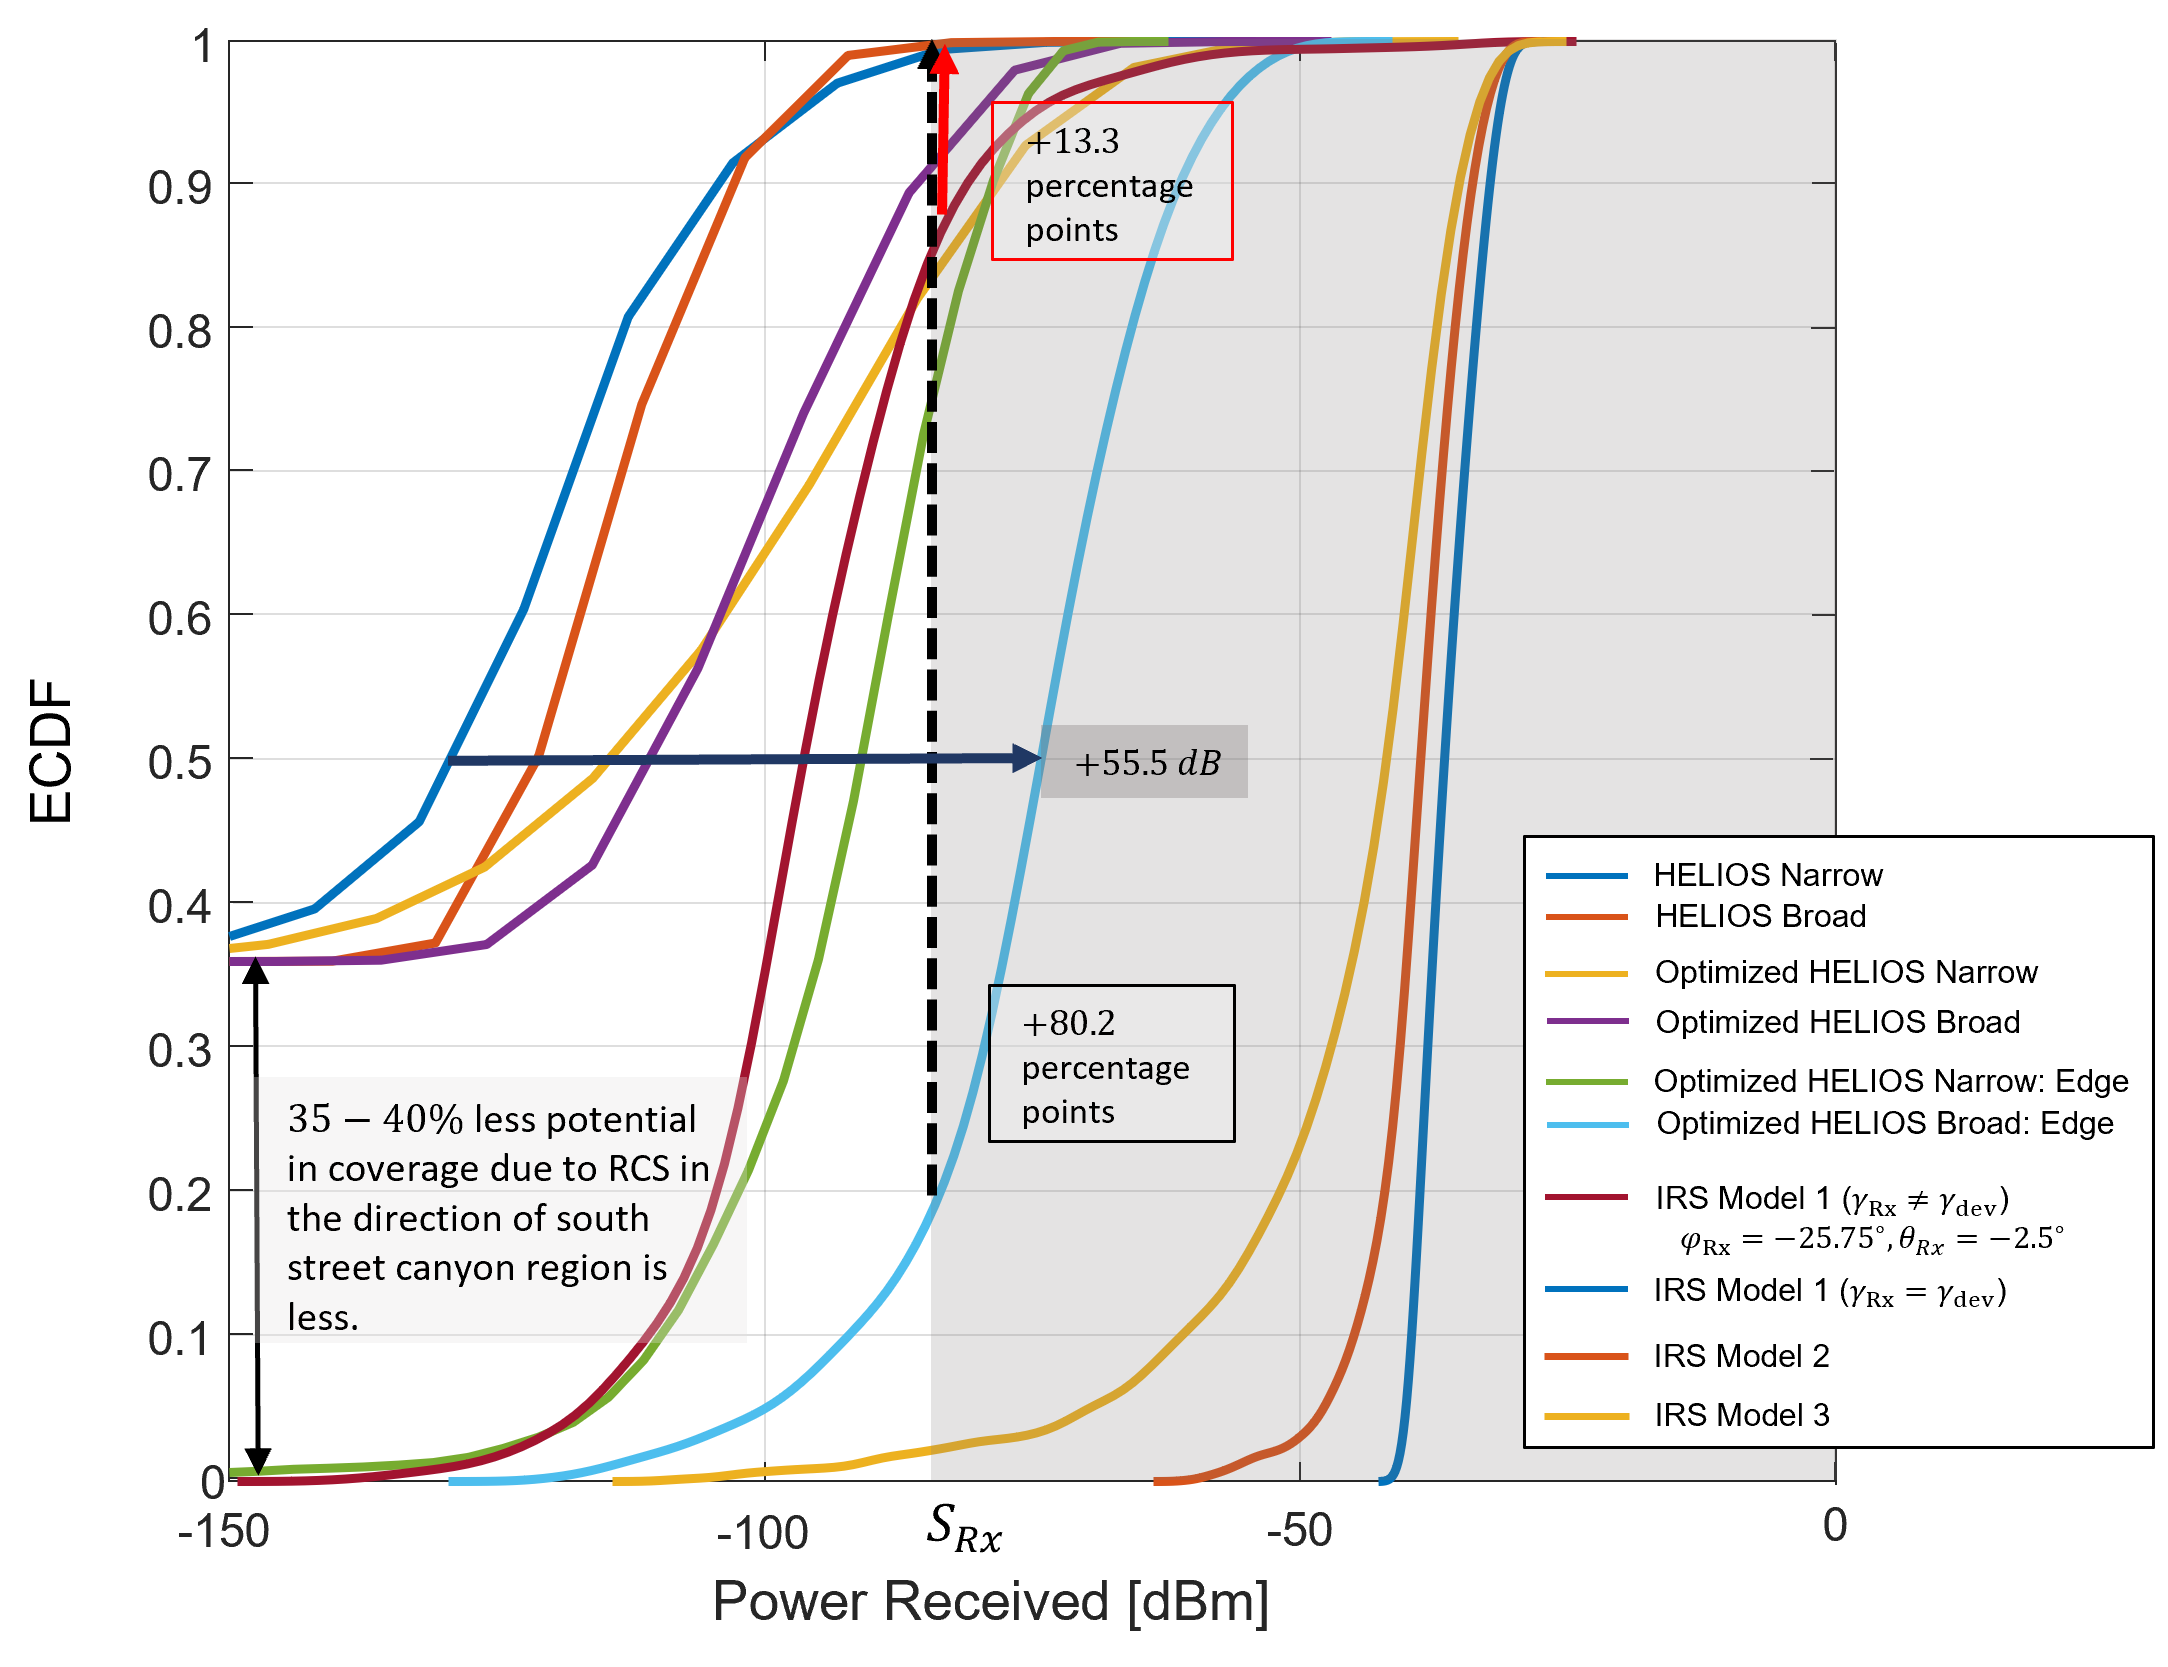
\includegraphics[width=1.0\linewidth]{images/Section 4 Images/Perfect_result_plot}
	\caption{ECDF plot depicting the power received in the south street canyon thus showcasing the performance of HELIOS and IRSs as predicted by analytical models, cf. \Cref{Model 1} (\cite{8936989, ntontin2021optimal, tang2020wireless}). Notably, the optimized broad beam HELIOS (geometry configuration + mounting position) shows more than 80.2 \% percentage coverage in our region of interest, while the fixed beam case of IRS model 1 exhibits 13.3 \% coverage. Our optimization increased the mean receive power by \SI{55.5}{\decibel} against \cite{Helios}. However, when compared to IRS which may reconfigure the reflection such that any position in the range is deliberately targeted, we still observe on average tens of dB of loss as well as reduced coverage.}
	\label{fig:Perfect_result_plot}
\end{figure}
However, we note that when fixing an IRS to a fixed configuration, we showed that HELIOS reflectors can perform better. An important takeaway from our case study is that reflector geometry and position optimization have a significant effect on signal strength and coverage. This considerable improvement highlights the effectiveness of our approach in enhancing signal propagation. Nonetheless, we point out the scope for more improvement as sophisticated algorithms should be considered for such purposes in the scope of hybrid network planning and HELIOS reflector customization processes.
\subsubsection{Case Study: Analyzing Behavior of Optimized HELIOS (Geometry Configuration + Mounting Position) Reflector on Frequency Variation}
Building upon the previous investigations conducted at \SI{28}{\giga\hertz} frequency, this study delves into analyzing the peak gain behavior for a frequency range from \SI{0.4}{\giga\hertz} to \SI{71}{\giga\hertz} in the steps of \SI{0.1}{\giga\hertz} for an optimized narrow beam HELIOS (Geometry configuration+ mounting position), see \Cref{Optimizing Connectivity with Different Reflector Positions}. \Cref{fig:Freq_vary_1} illustrates the reflector gain behavior across this spectrum, revealing three distinct regions: (a) $f\in [0.4:2.0] \si{\giga\hertz}$, where lower gains are observed at lower frequencies. (b) $f\in [2.0:38.7] \si{\giga\hertz}$ shows higher gains indicating optimal performance of the reflectors. (c) $f\in [38.7:71] \si{\giga\hertz}$ is characterized by higher frequencies, a noticeable loss in gain exceeding \SI{5}{\decibel} is observed.

\Cref{fig:Freq_vary_2} depicts the peak gains achieved in the green color-coded region, i.e., a peak gain value of \SI{31.8}{\decibel} at \SI{2.8}{\giga\hertz} being the highest, with \SI{31.0}{\decibel} at \SI{9}{\giga\hertz}, \SI{15.1}{\giga\hertz}, and \SI{21.1}{\giga\hertz} being the second highest peaks. Notably, at \SI{28}{\giga\hertz} frequency, we observe a peak gain of \SI{29}{\decibel} which is the same as the results we got from \Cref{Optimizing Connectivity with Different Reflector Positions}. The RCS gain and receive power behavior at \SI{2}{\giga\hertz}, \SI{28}{\giga\hertz}, and \SI{48}{\giga\hertz} frequency is seen in \Cref{fig:Freq_vary_2}. The three frequencies in the figure belongs to each of the three distinct regions in \Cref{fig:Freq_vary_1}. Initially, we observe that the near-field region (white-colored region), increases as the frequency increases. This direct dependency on frequency can be observed from \Cref{Near-field}. 
\begin{figure}[H]
	\centering
	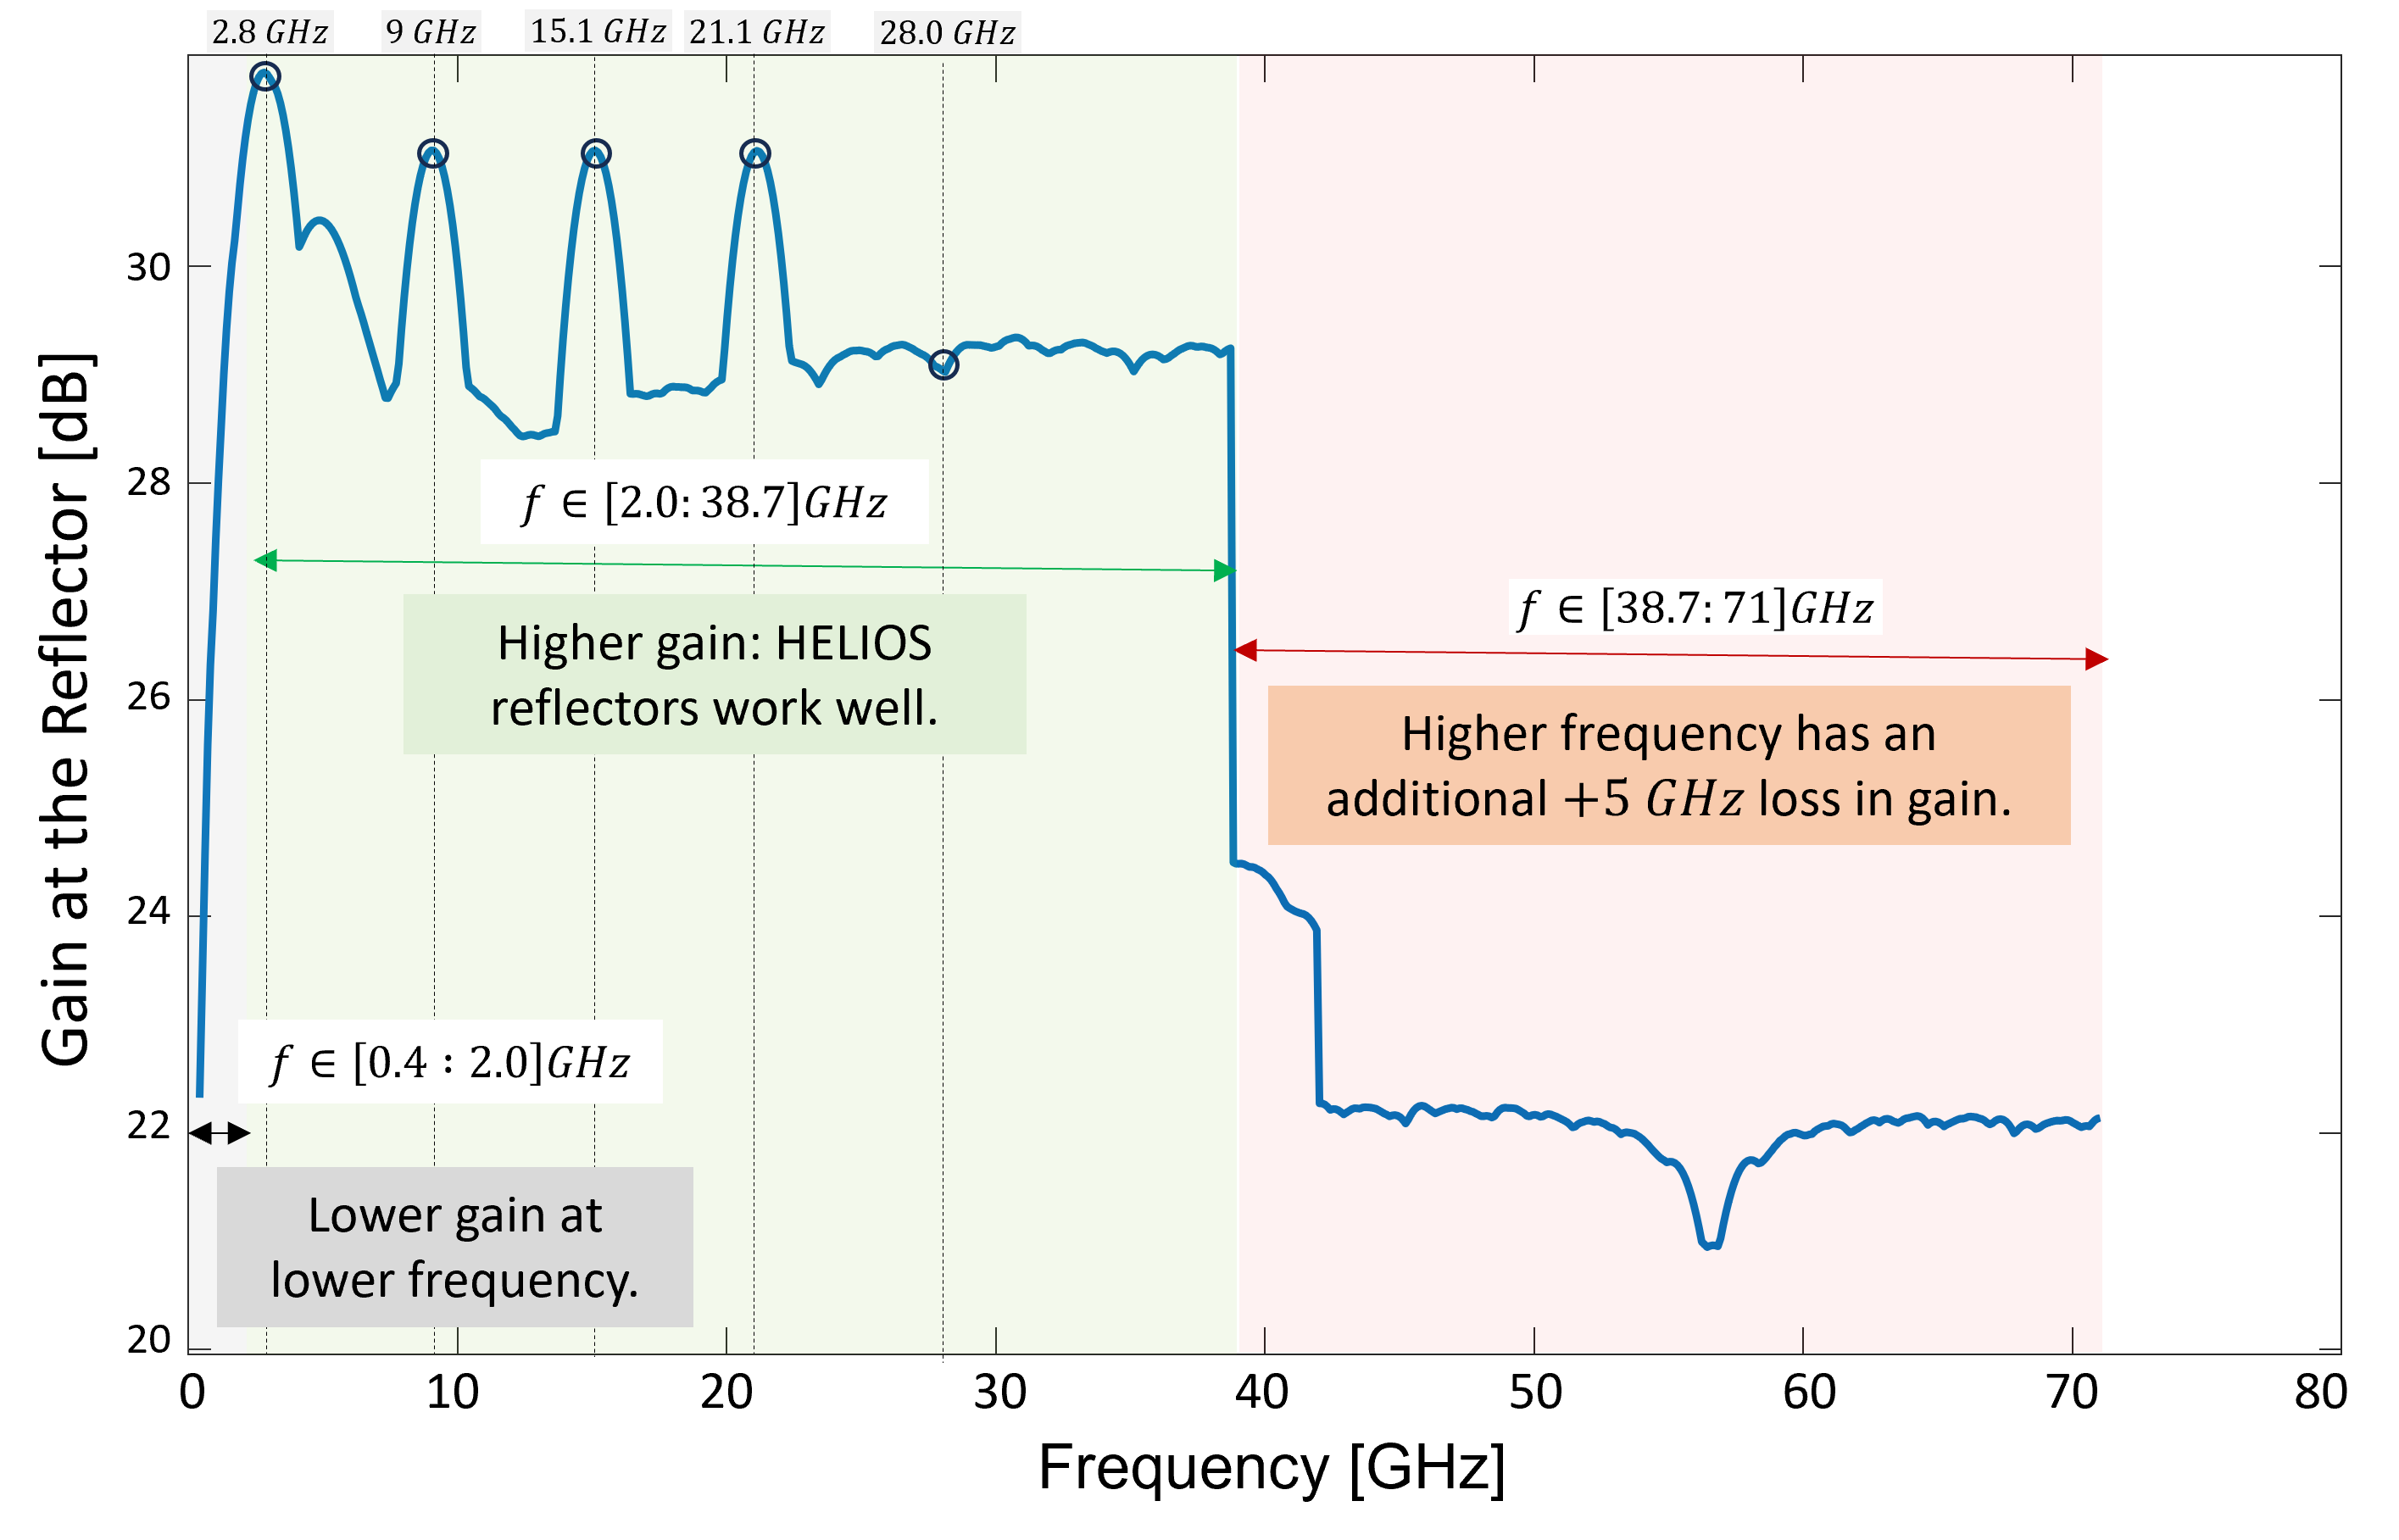
\includegraphics[width=0.9\linewidth]{images/Section 4 Images/Freq_vary_1}
	\caption{Variation of peak gain for span in frequency range $f\in [0.4:71] \si{\giga\hertz}$ in the steps of \SI{0.1}{\giga\hertz}. Three distinct frequency ranges depend on the peak gain values as depicted with color coding. Higher gains are observed in the green region showcasing the better performance of the HELIOS reflectors in this frequency range.}
	\label{fig:Freq_vary_1}
\end{figure}
\begin{figure}[tb]
	\centering
	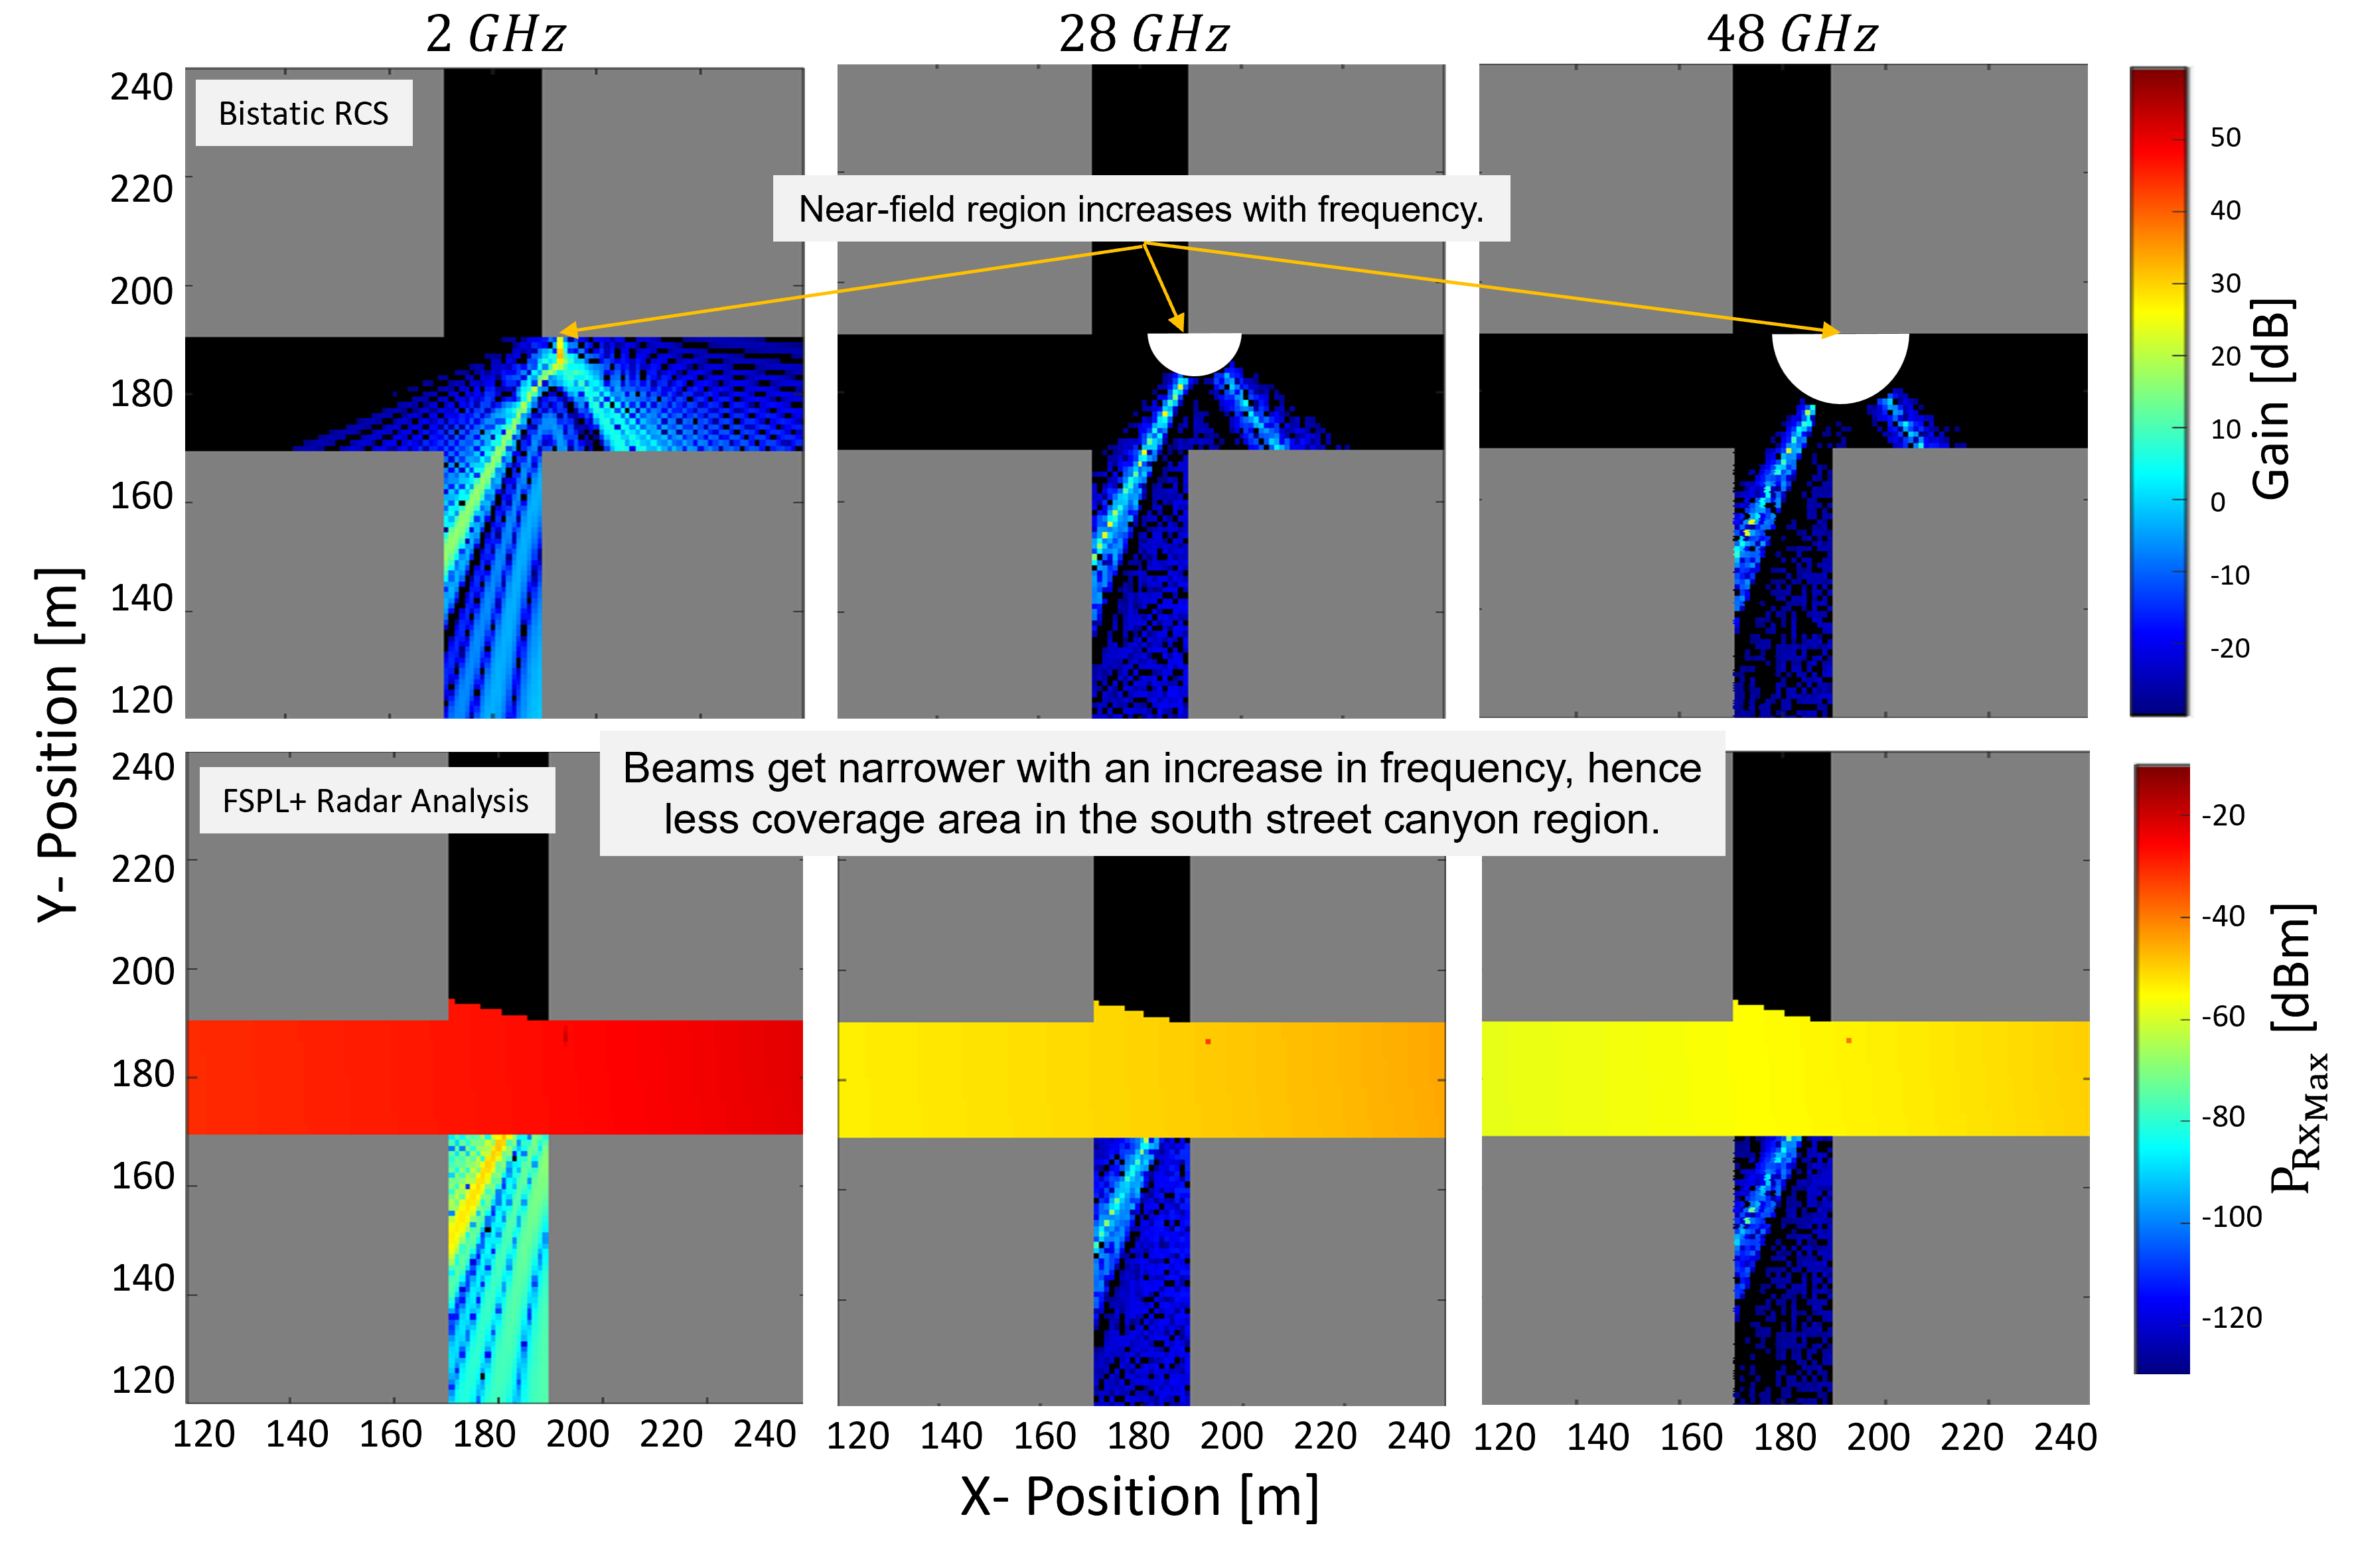
\includegraphics[width=0.95\linewidth]{images/Section 4 Images/Freq_vary_2}
	\caption{RCS comparison of optimized narrow beam HELIOS (Geometry configuration+ mounting position) at \SI{2}{\giga\hertz}, \SI{28}{\giga\hertz}, and \SI{48}{\giga\hertz} frequency in an urban scenario depicting the gain in \si{\decibel} (top row) and maximum power received in \si{\decibel}m (bottom row).}
	\label{fig:Freq_vary_2}
\end{figure} 

Referring to \Cref{Eq:HELIOS_module}, the direct dependency of frequency ($f=\frac{2\cdot \pi}{k}$) inside the $\sinc$ function of a HELIOS module, due to which the value inside the $\sinc$ function reduces as frequency increases. Thus leading to the narrow beam, as observed in \Cref{fig:Freq_vary_2} from \SI{2}{\giga\hertz} to \SI{48}{\giga\hertz}. The coverage area in the south street canyon region accounts for \num{97.0}\%, \num{23.0}\%, and \num{6}\% for models operating with \SI{2}{\giga\hertz}, \SI{28}{\giga\hertz}, and \SI{48}{\giga\hertz}, respectively. A drastic decrease in coverage area by almost \num{91}\% occurs as the frequency increases. 
\subsection{Sensitivity Point: HELIOS performance with UMi-Radar Equation}\label{Interpreting Different Channel Models}
The above study items have used FSPL channel models in an urban setting. It is imperative to acknowledge, nevertheless, that other channel models like the 3GPP UMi and others are typically a better choice for such. The basic formula for representing radar behavior in different contexts is found in \Cref{fig:FSPL_Radar}. Using the insights from \Cref{FSPL_delta}, we now explicitly examine the behavior when coupled with different propagation models. To use these models together with the reflecting surface, the channel is split into two parts: LOS and NLOS region as mentioned in \Cref{UMi scenario}, unlike FSPL which considers LOS paths only. Using the factor $\Delta D_{ChainedFSPL}$ as introduced previously in \Cref{Baseline Performance of FSPL Model}, we thus extend the UMi channel model to a radar equation-like formula as follows:
\begin{equation}
	\begin{aligned}
		PL_{UMi_{Radar}}(r_{Tx,Ref},r_{Ref,Rx},f,\sigma_{Meta},G_{Tx}, G_{Rx})&=PL_{UMi}(G_{Tx}, r_{Tx,Ref},f)+PL_{UMi}(G_{Rx}, r_{Ref,Rx},f)+\\ &\sigma_{Meta}-\Delta D_{UMi}
	\end{aligned}
\end{equation}
\begin{equation} \label{Umi_delta}
	\Delta D_{UMi}= 52\cdot log_{10}(4 \cdot \pi)- 20\cdot log_{10}(c)+20\cdot log_{10}(f).
\end{equation}

Although resembling the $\Delta D_{ChainedFSPL}$ parameter used in FSPL, it incorporates a distinct offset of $52\cdot log_{10}(4 \cdot \pi)$ as seen in \Cref{Umi_delta}. The rationale behind selecting this changed offset lies in its ability to account for scenarios where reflectors are situated near the transmitter, typically within a few tens of meters. This offset ensures that the radar path loss neither exceeds the NLOS value nor proceeds LOS value, especially when the reflector is located near the transmitter. Using the above equation, \Cref{fig:UMi_Radar} gives a brief comparison of predicted and radar path losses for an arbitrary scenario assuming $\sigma_{Meta}=\SI{0}{\decibel}$ and the reflector is located at \SI{50}{\meter}. The same assumptions were carried out for FSPL in \Cref{fig:FSPL_Radar}.

The minimum range of $r_{Tx, Rx}$ as seen from \Cref{UMi scenario} is \SI{10}{\meter} \cite{ETSI}. Observing the figure, there is a noticeable shift in the radar curve of about \SI{13}{\decibel}, at the reflector's assigned position with an ideal offset of $52\cdot log_{10}(4 \cdot \pi)$. Having seen the new radar-like performance, we now consider the HELIOS deployment from \Cref{Optimizing Connectivity with Different Reflector Positions} and consider the attained connectivity boost, see \Cref{fig:UMi_Helios_urban}.

\begin{figure}[H]
	\centering
	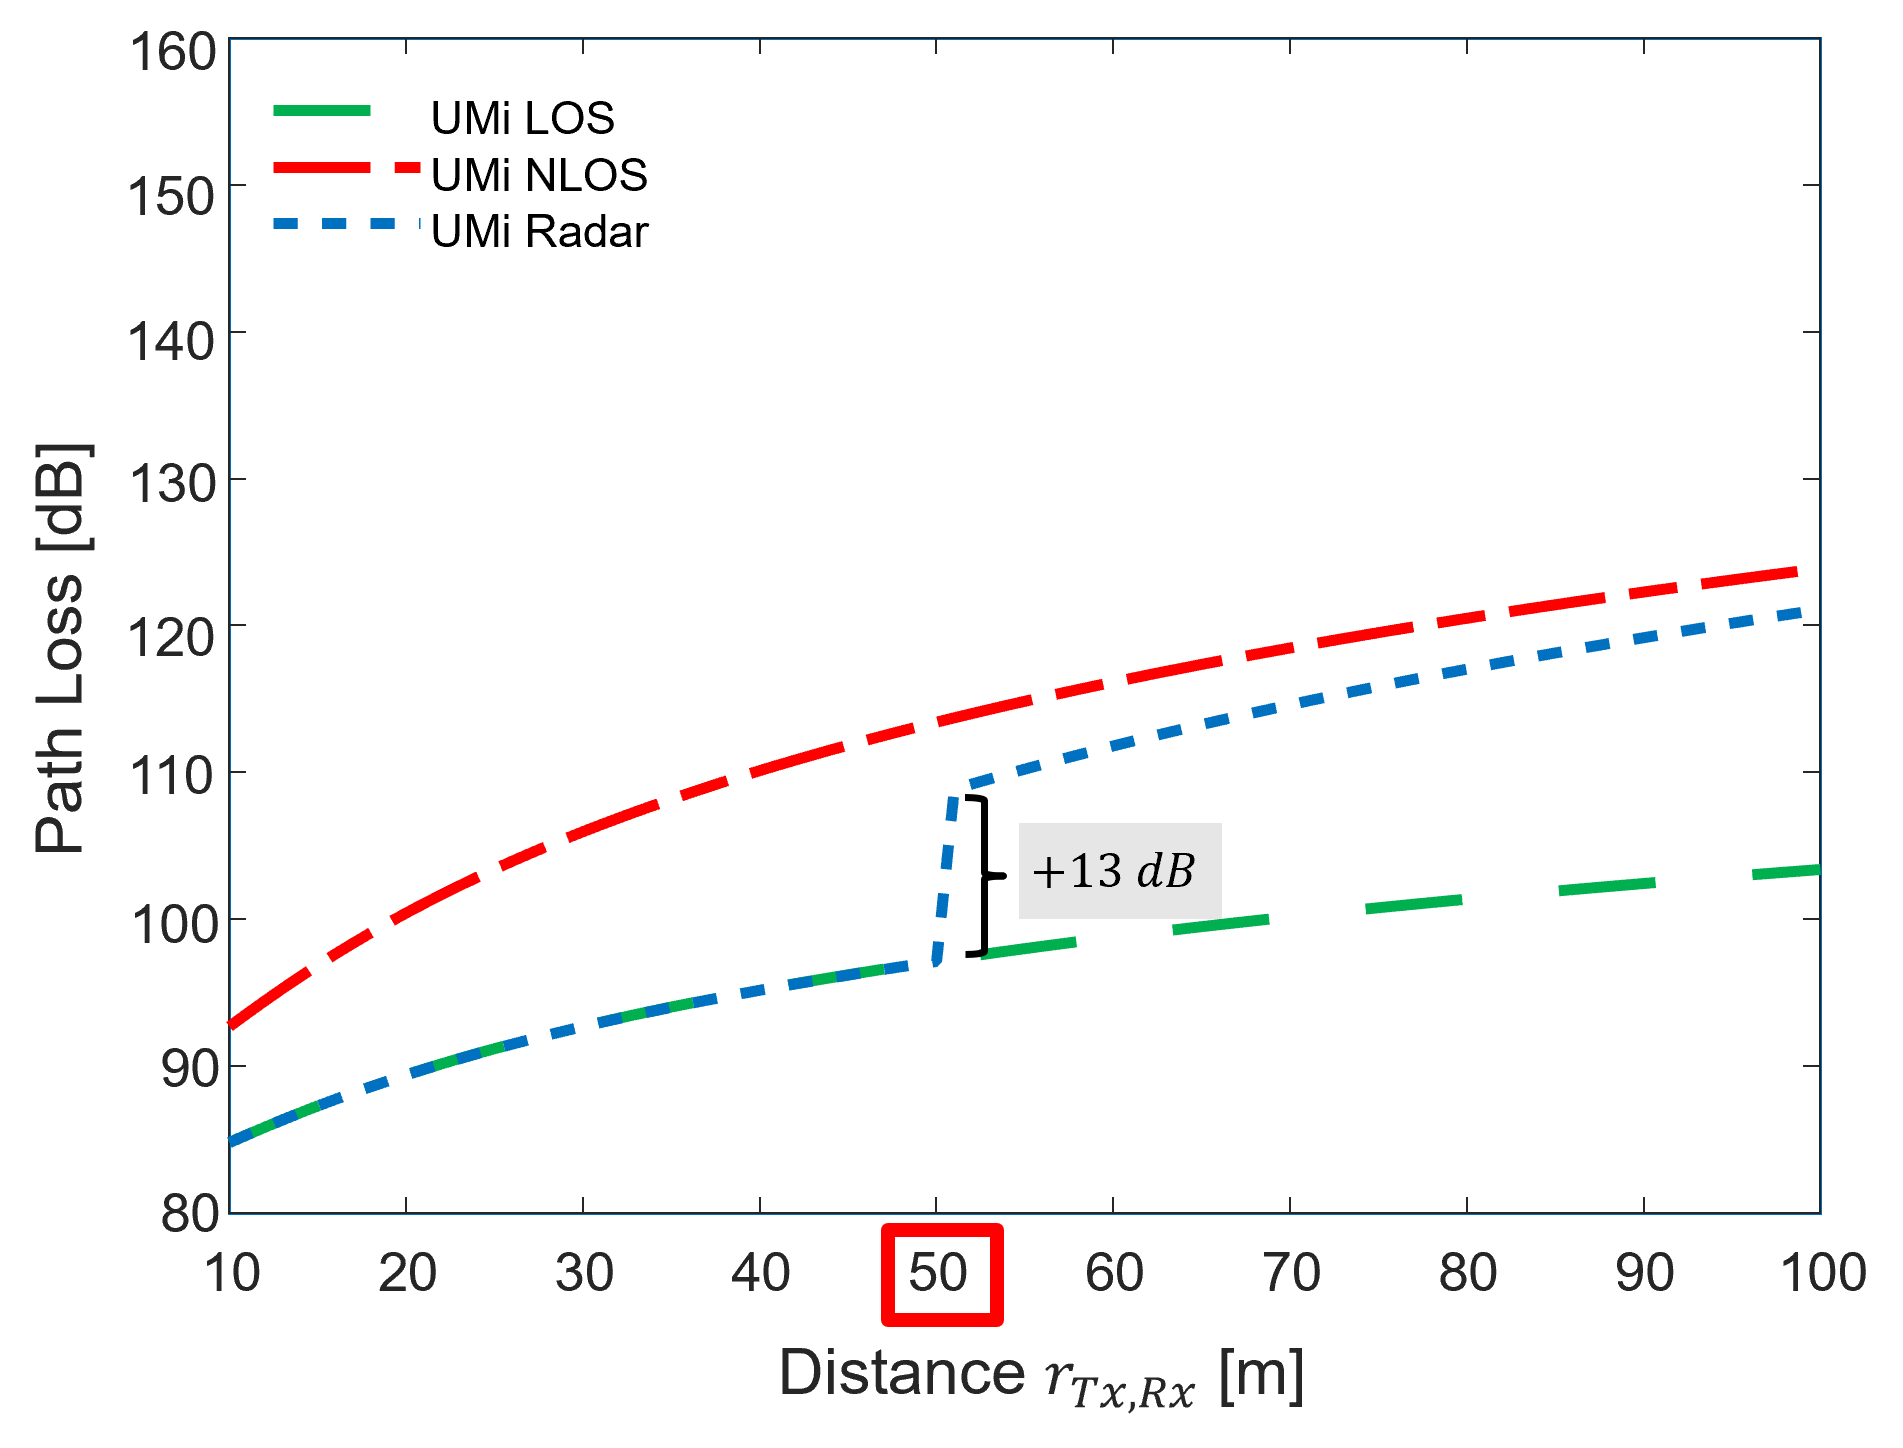
\includegraphics[width=0.8\linewidth]{images/Section 4 Images/UMi_Radar1}
	\caption{Comparison between predicted LOS, NLOS path loss of UMi channel model, and the radar equation over the total distance between Tx and Rx. For the radar curve, we assume LOS connectivity for the first \SI{50}{\meter}, as the reflector is located at \SI{50}{\meter} from Tx. Thereafter, it follows the radar path with $\sigma_{Meta}=\SI{0}{\decibel}$ and $r_{Tx, Rx}=r_{Ref, Rx}$.}
	\label{fig:UMi_Radar}
\end{figure}
\begin{figure}[H]
	\centering
	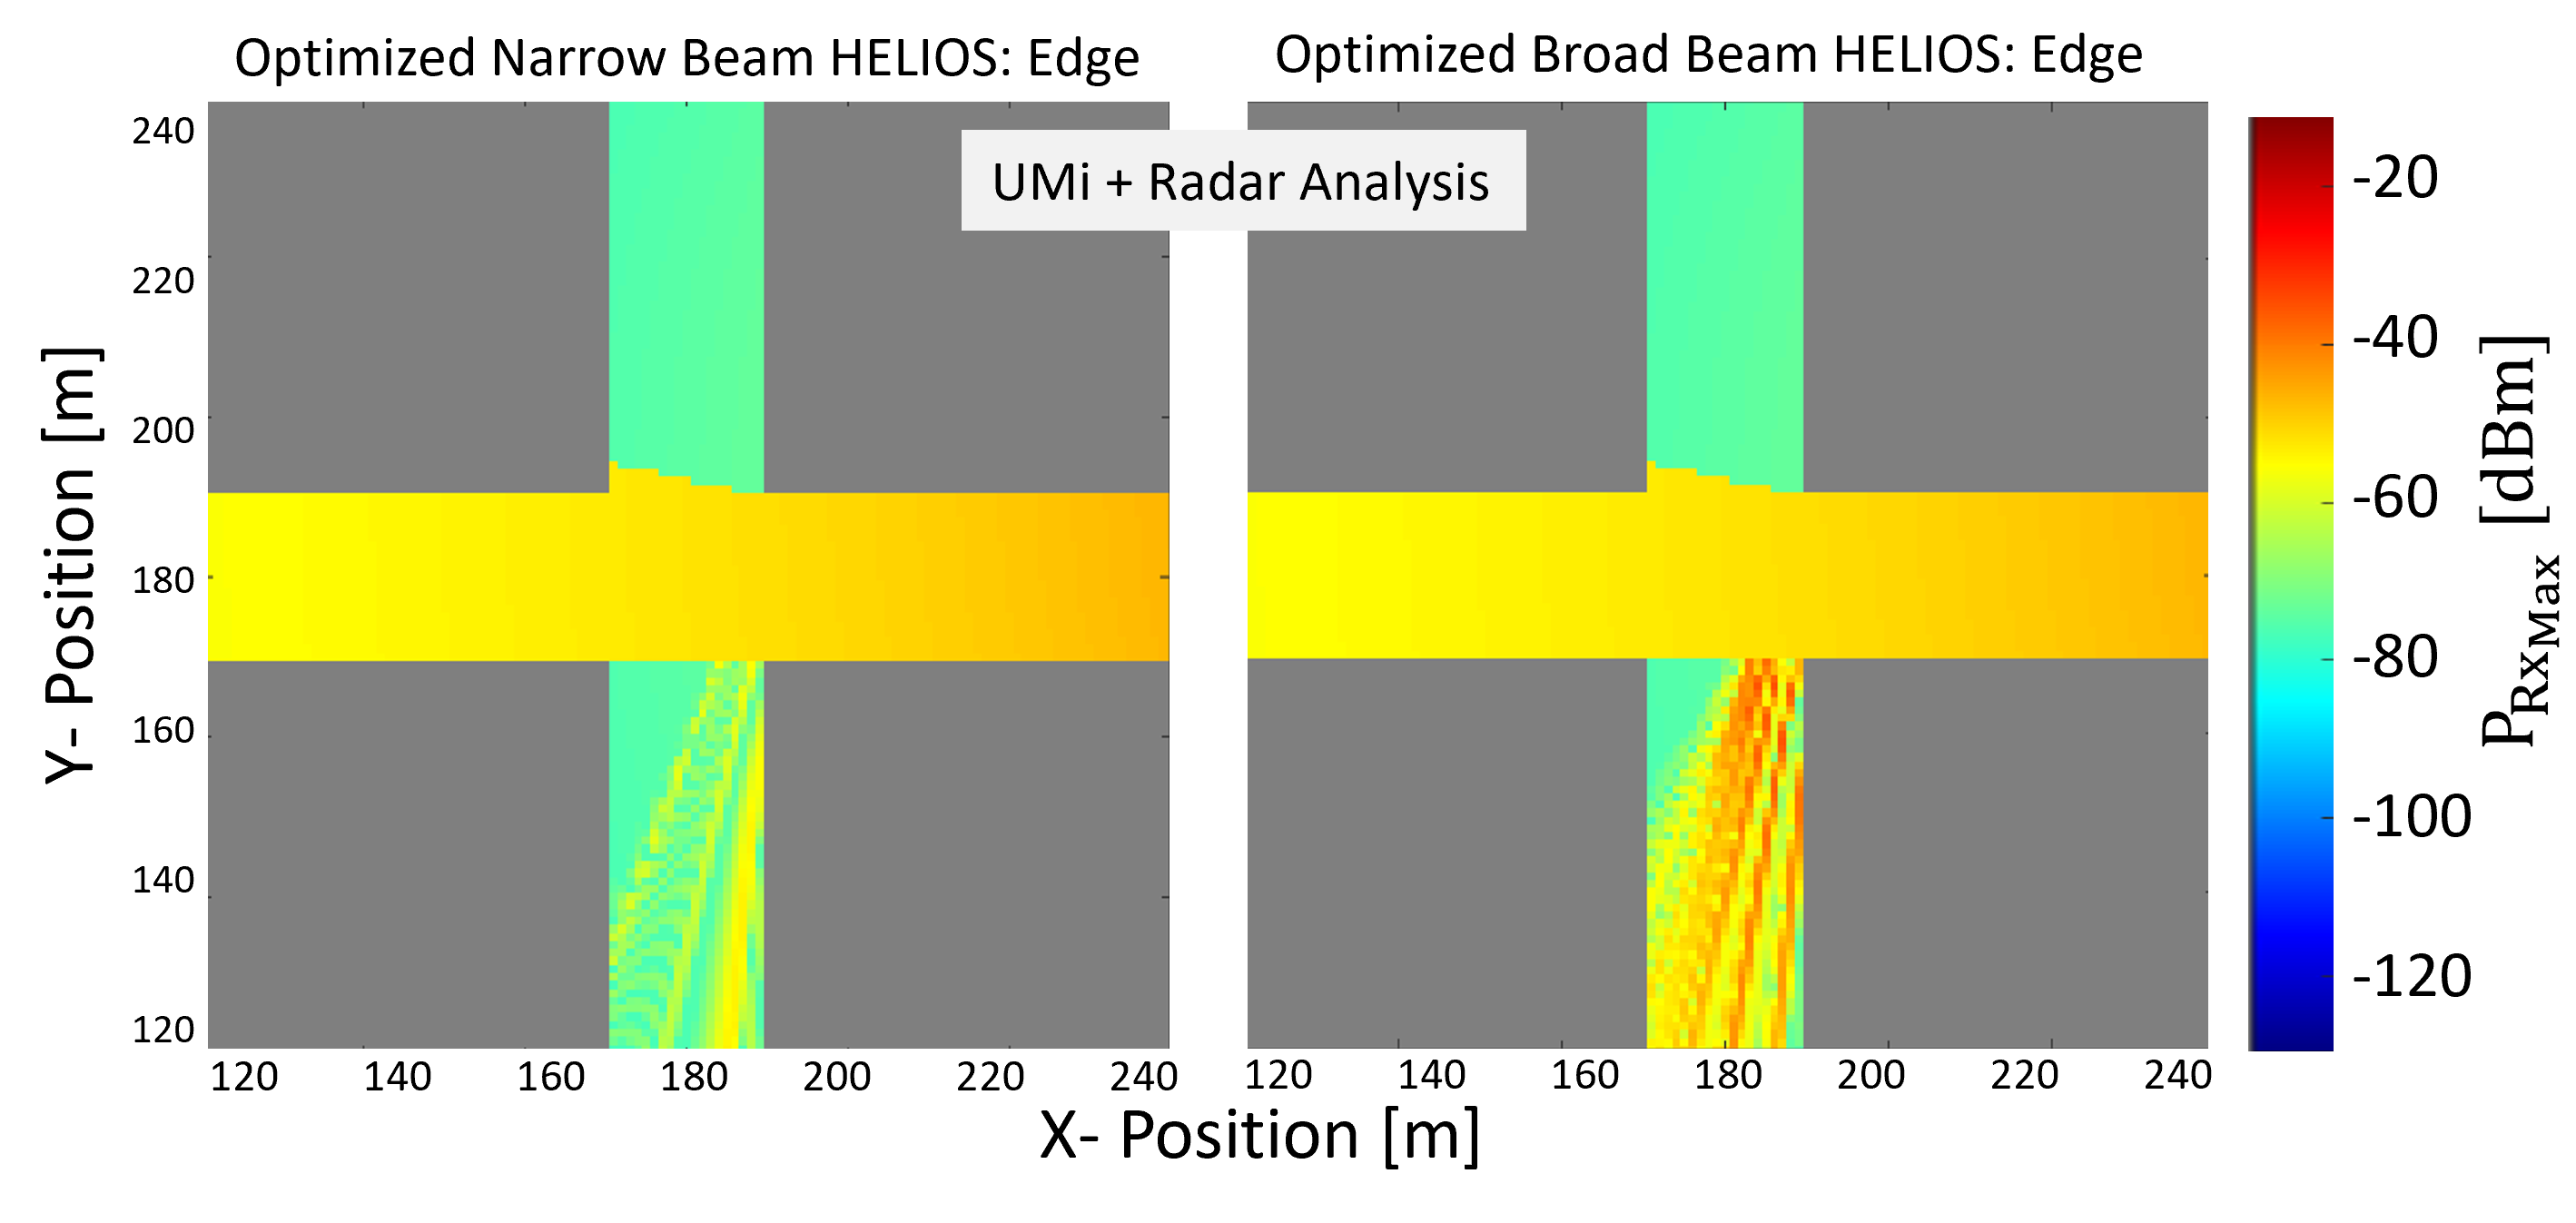
\includegraphics[width=0.83\linewidth]{images/Section 4 Images/UMi_Helios_urban}
	\caption{UMi channel model RCS comparison of optimized narrow beam HELIOS (left column) and broad beams HELIOS (right column) in urban scenario depicting maximum power received in \si{\decibel}m. The parameters are considered from \Cref{Table:Urban case study} at \SI{28}{\giga\hertz} frequency with the optimized slope angles at the edge of the building, see	\Cref{Optimizing Connectivity with Different Reflector Positions}.}
	\label{fig:UMi_Helios_urban}
\end{figure}
We find additional connectivity to the NLOS region using the UMi channel model in an urban scenario. When compared to the results in \Cref{Optimizing Connectivity with Different Reflector Positions}, the coverage area in the south street canyon enhanced by more than \num{60} \%, and \num{19.3} \% with optimized narrow and broad beam HELIOS, respectively. Similar to the deployment in \Cref{Comparing Passive Analytical Model to Active IRS Models} and for the same deployment of reflectors, we extend our study with new IRS channel models \Cref{coordinate systems}. Comparing the results between \Cref{fig:UMi_IRS_MOdel1}, and \Cref{fig:urbanscenario_IRSmodel1s}, we achieve enhanced coverage area with fixed beam case of IRS model by \num{78.1} \%, whereas the other case dynamic beam provides \num{100} \% coverage. 

\begin{figure}[H]
	\centering
	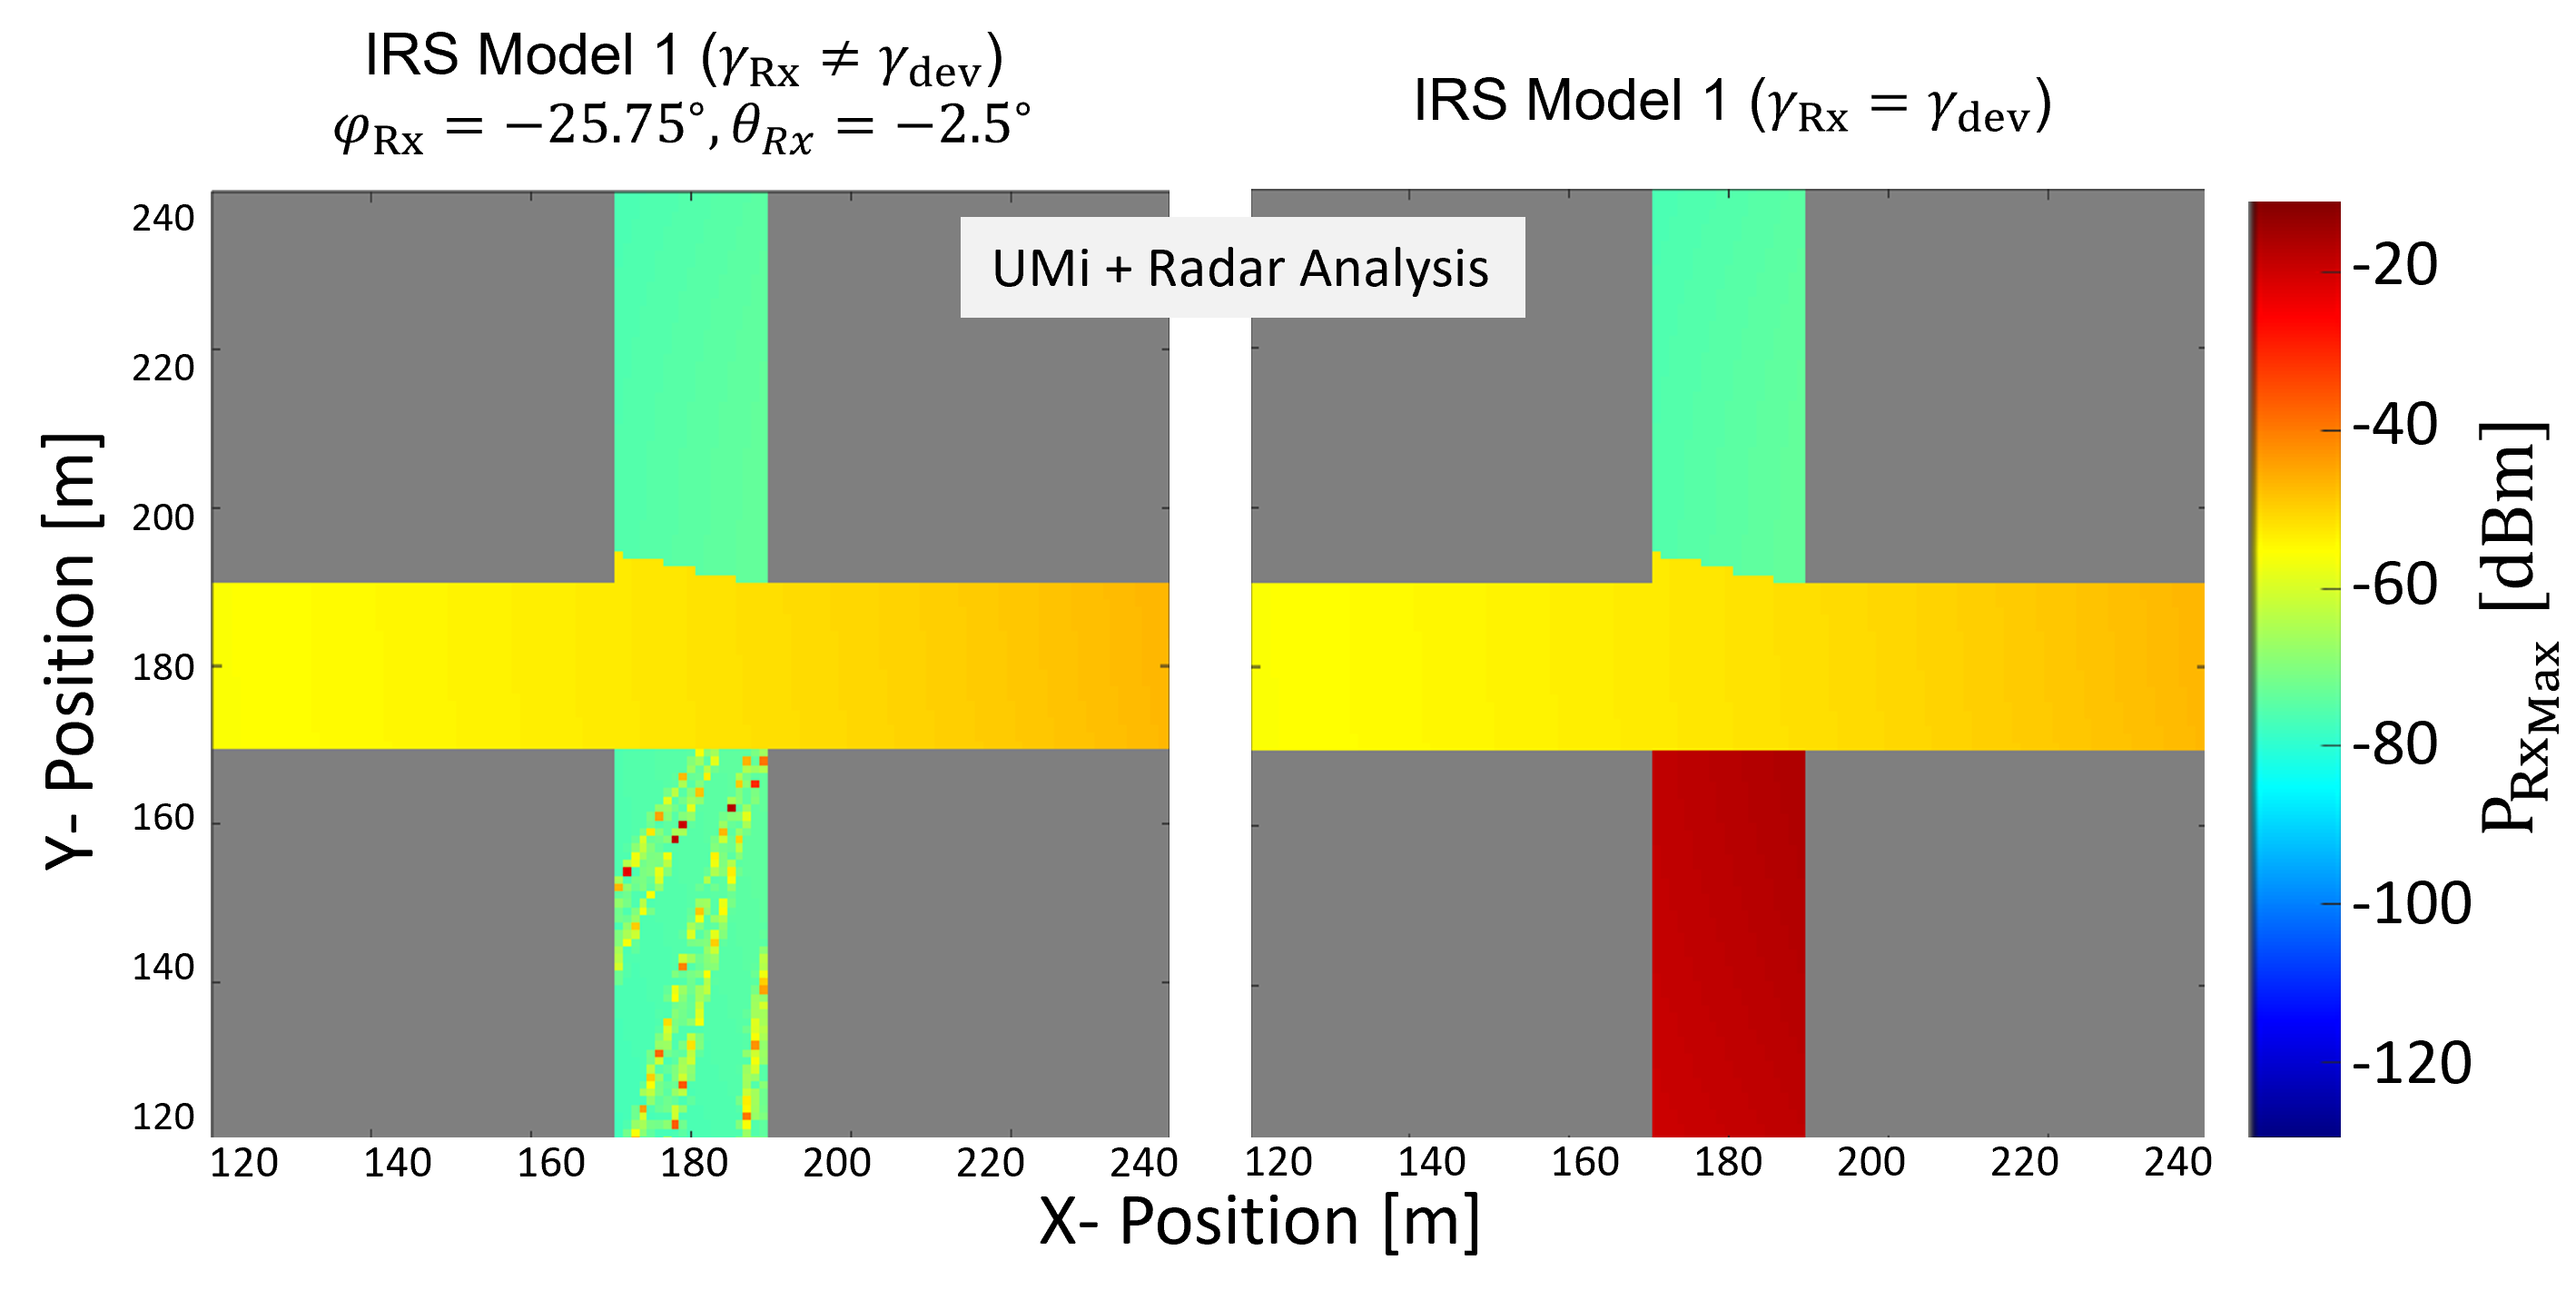
\includegraphics[width=0.83\linewidth]{images/Section 4 Images/UMi_IRS_MOdel1}
	\caption{UMi channel model RCS comparison of two cases of IRS model 1 (\Cref{Model 1}): fixed beam case on the left column and dynamic beam on the right column in an urban scenario depicting maximum power received in \si{\decibel}m. The parameters are considered from \Cref{Table:Urban case study} at \SI{28}{\giga\hertz} frequency with the optimized slope angles at the edge of the building, see \Cref{Optimizing Connectivity with Different Reflector Positions}.}
	\label{fig:UMi_IRS_MOdel1}
\end{figure}
\begin{figure}[H]
	\centering
	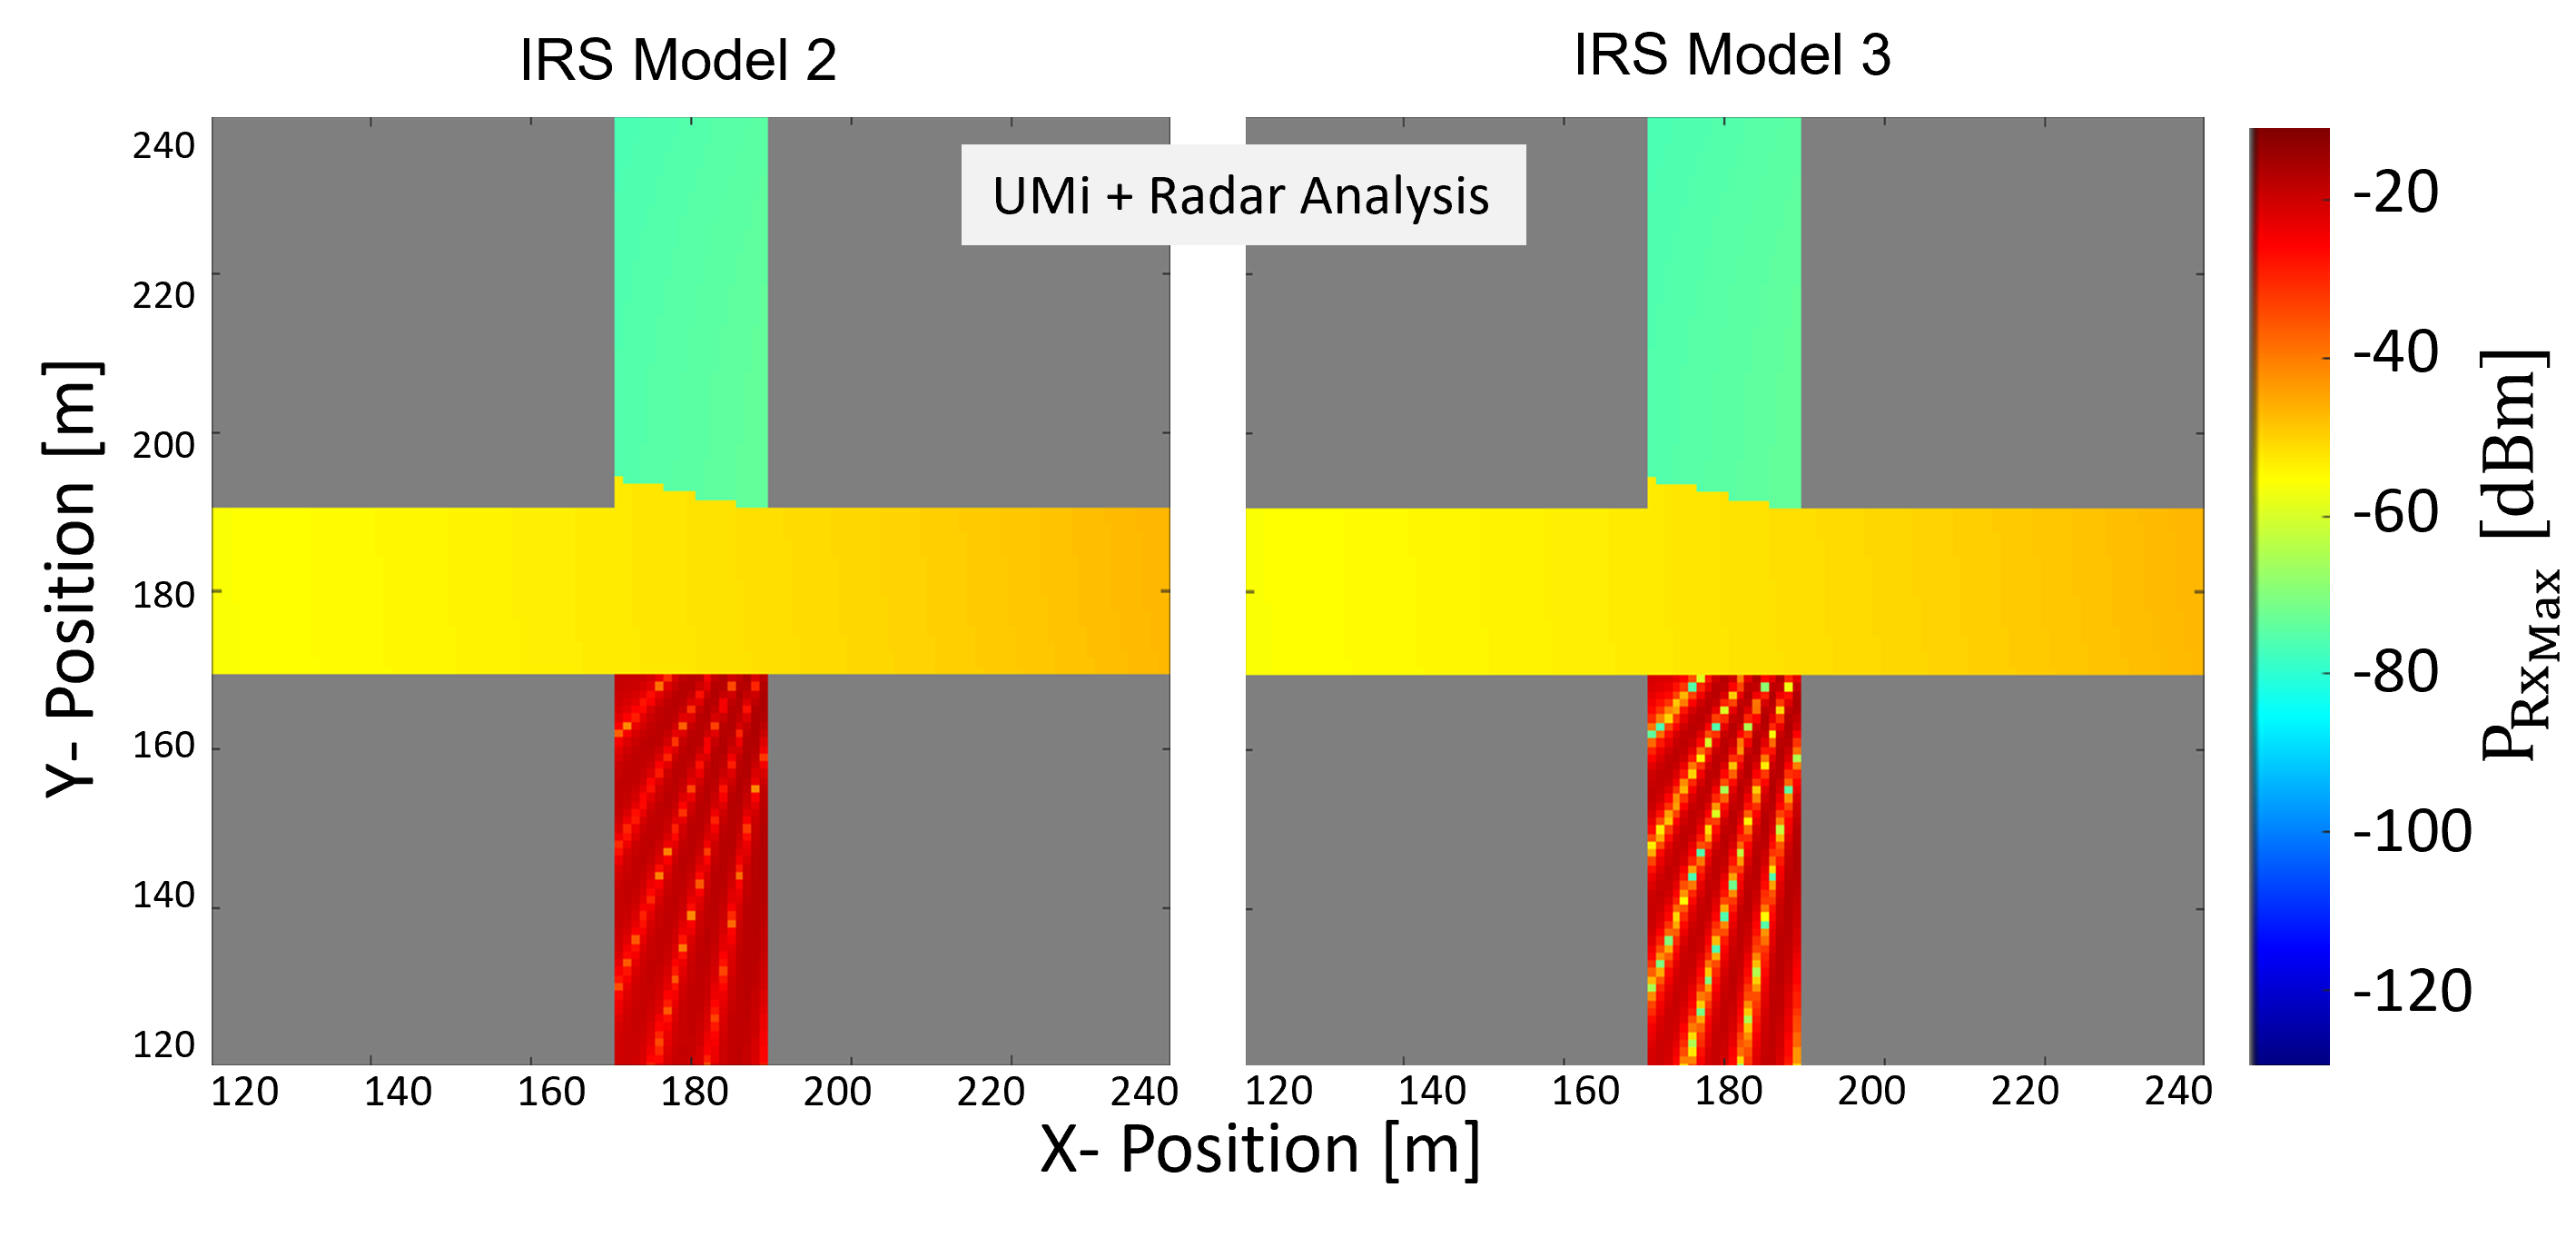
\includegraphics[width=0.83\linewidth]{images/Section 4 Images/UMi_IRS_MOdel2_3}
	\caption{UMi channel model RCS comparison of two IRS models \Cref{Model 3} in urban scenario depicting maximum power received in \si{\decibel}m. The parameters are considered from \Cref{Table:Urban case study} at \SI{28}{\giga\hertz} frequency with the optimized slope angles at the edge of the building, see \Cref{Optimizing Connectivity with Different Reflector Positions}.}
	\label{fig:UMi_IRS_MOdel2_3}
\end{figure}
\begin{figure}[H]
	\centering
	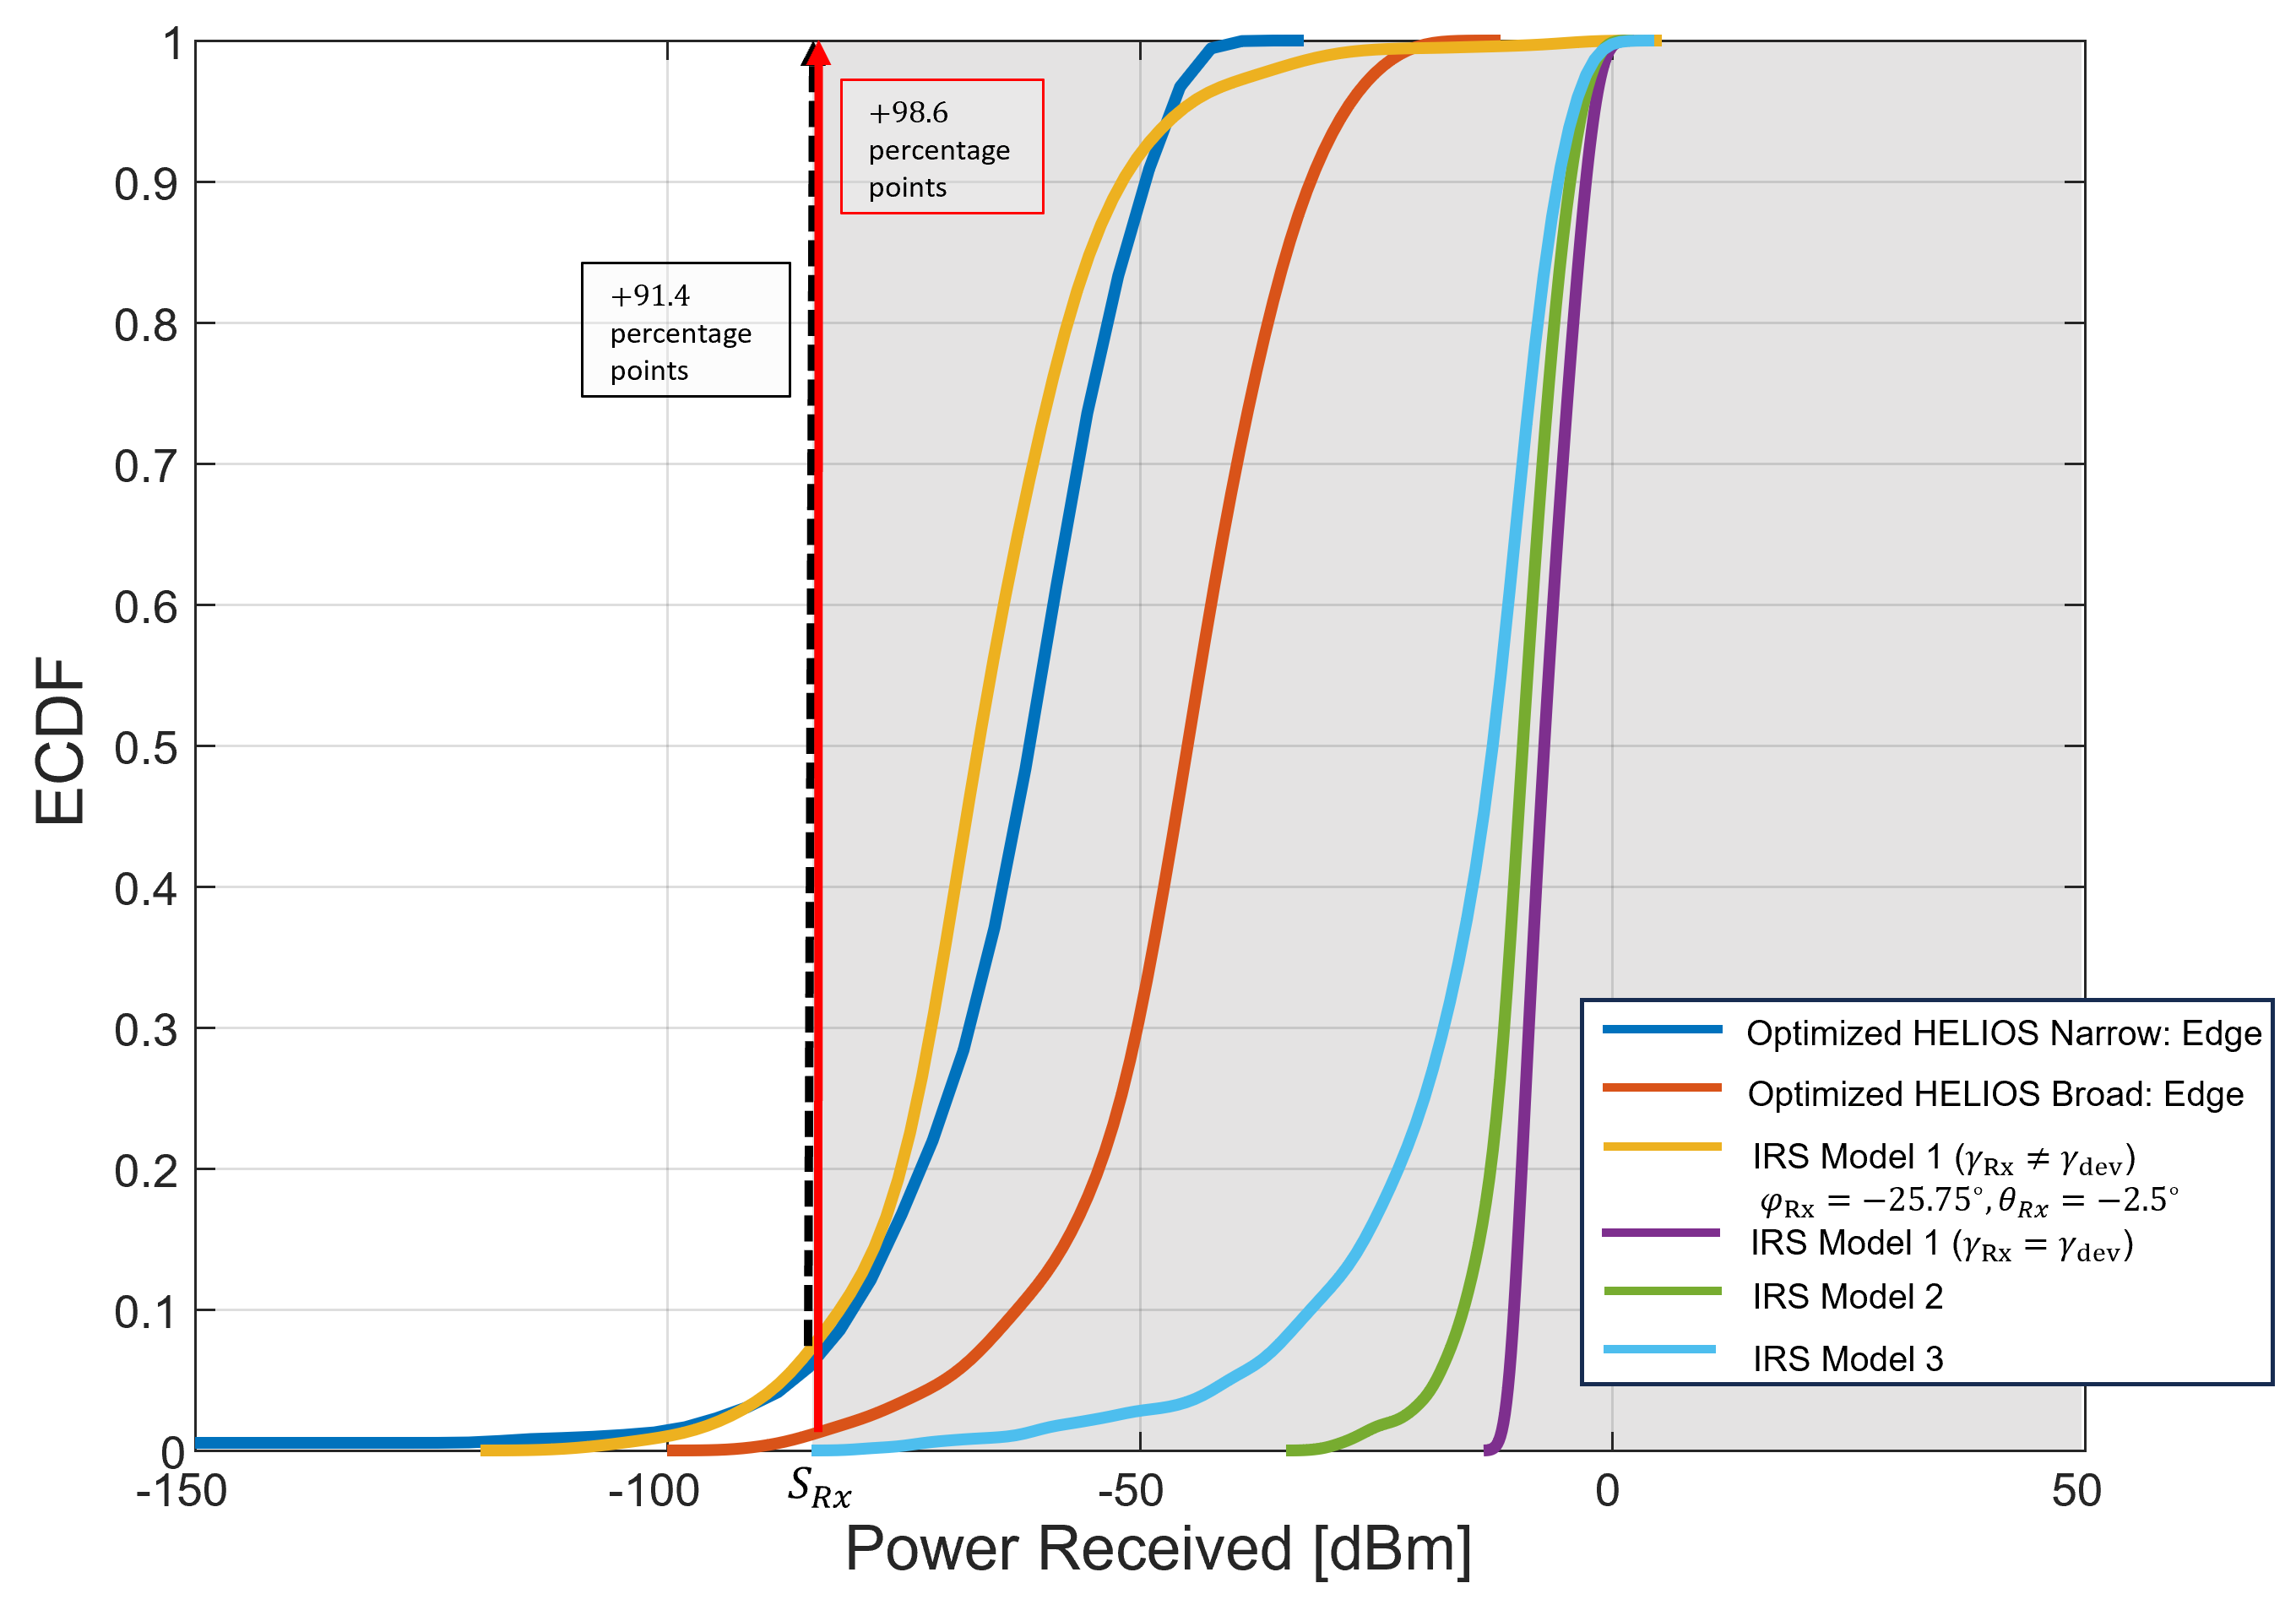
\includegraphics[width=0.9\linewidth]{images/Section 4 Images/Perfect_result_plot_UMi}
	\caption{ECDF plot depicting the power received in the south street canyon in \si{\decibel}m by UMi channel model in urban scenario, highlighting the performance and coverage by our optimized HELIOS analytical model and IRS models \cite{8936989, ntontin2021optimal, tang2020wireless} in \Cref{Model 1}. Notably, optimized HELIOS broad beam around the edge of the building shows more than 98.6 \% percentage coverage in our region of interest, while fixed beam case of IRS model 1 exhibits 91.4 \% coverage.}
	\label{fig:Perfect_result_plot_UMi}
\end{figure}
The comparison of \Cref{fig:UMi_IRS_MOdel2_3}, and \Cref{fig:urbanscenario_IRSmodel2_3}, we achieve \num{100} \% coverage in south street canyon using UMi channel modeling. In the above figure, the power is radiating in the direction of south street canyon with a coverage area of around \num{92.5} \% with narrow beam and \num{98.6} \% with broad beam HELIOS (geometry configuration + mounting position) (see \Cref{fig:UMi_IRS_MOdel1}). Whereas active IRS models show a coverage area of around \num{100} \% in all the cases. Like in \Cref{Comparing Passive Analytical Model to Active IRS Models}, we bundle the results from \Cref{fig:UMi_Helios_urban}, \Cref{fig:UMi_IRS_MOdel1}, and \Cref{fig:UMi_IRS_MOdel2_3} in \Cref{fig:Perfect_result_plot_UMi} depicting the respective receive power ECDFs. Notably, the coverage area in the south street canyon by almost all reflecting surfaces of the curves approaches \num{100} \%, contrasting to the ECDF plot in \Cref{fig:Perfect_result_plot} with FSPL channel model. These much more optimistic results come from the UMi channel's behavior to account for the complex interactions found in urban environments, such as reflections, diffraction, and scattering. This leads to a more accurate representation of signal propagation in intricate urban landscapes. In contrast, FSPL oversimplifies the scenario by ignoring these environmental details, which results in an underprediction for the connectivity, However, if taken as the basis for network planning, this will ensure over-provisioning by network operators (using BSs and metasurfaces) which would be of interest for the users.
\section{Outlook on Future Arbitrarily-Shaped HELIOS Reflecting Surfaces}\label{Outlook on Future Arbitrarily-Shaped HELIOS Reflecting Surfaces}
We have used the simulation program in our endeavor to optimize reflector designs, and we have used both squared and rectangular reflecting surfaces. Moving away from such flat reflecting surfaces, e.g., by introducing curvature, cf. \cite{Helios}, such a HELIOS reflector is represented in the form of triangulated geometry. The use of a large number of triangle surface patches for complex 3D objects is typical in computer graphics and a key part of CAD programs and related file formats such as *.stl. To put our analytical model to use for more complex reflecting surface geometries, we briefly study to what regards the behavior changes and what this would mean for our analytical model. 

One of the main differences between the triangle and rectangles is the surface area size. The area of a rectangle, denoted by $A_{rect}$, can be found by multiplying its sides $a\cdot b$. In contrast, the area of a triangle is just $A_{tri} = \frac{1}{2}\cdot (a\cdot b)$. Considering that the RCS is proportional to the area squared, see \Cref{Eq:HELIOS_array}, one would expect a \SI{6}{\decibel} loss in peak RCS. However, when using two triangles to construct a rectangle from two triangles, these differences should be remedied and the overall RCS pattern should match our current analytical model. In the following, we assess how the RCS pattern for triangular surface patches differs from the one from a rectangular surface. We consider four different triangles that fit into the space spanned by a quadratic surface patch of size $a=b=\SI{0.1}{\meter}$, see top of \Cref{fig:Triangle_square}. As a result, different edge alignments around the surface patches are realized. They are highlighted in black when parallel to the $z$-axis, yellow when 
\begin{figure}[tb]
	\centering
	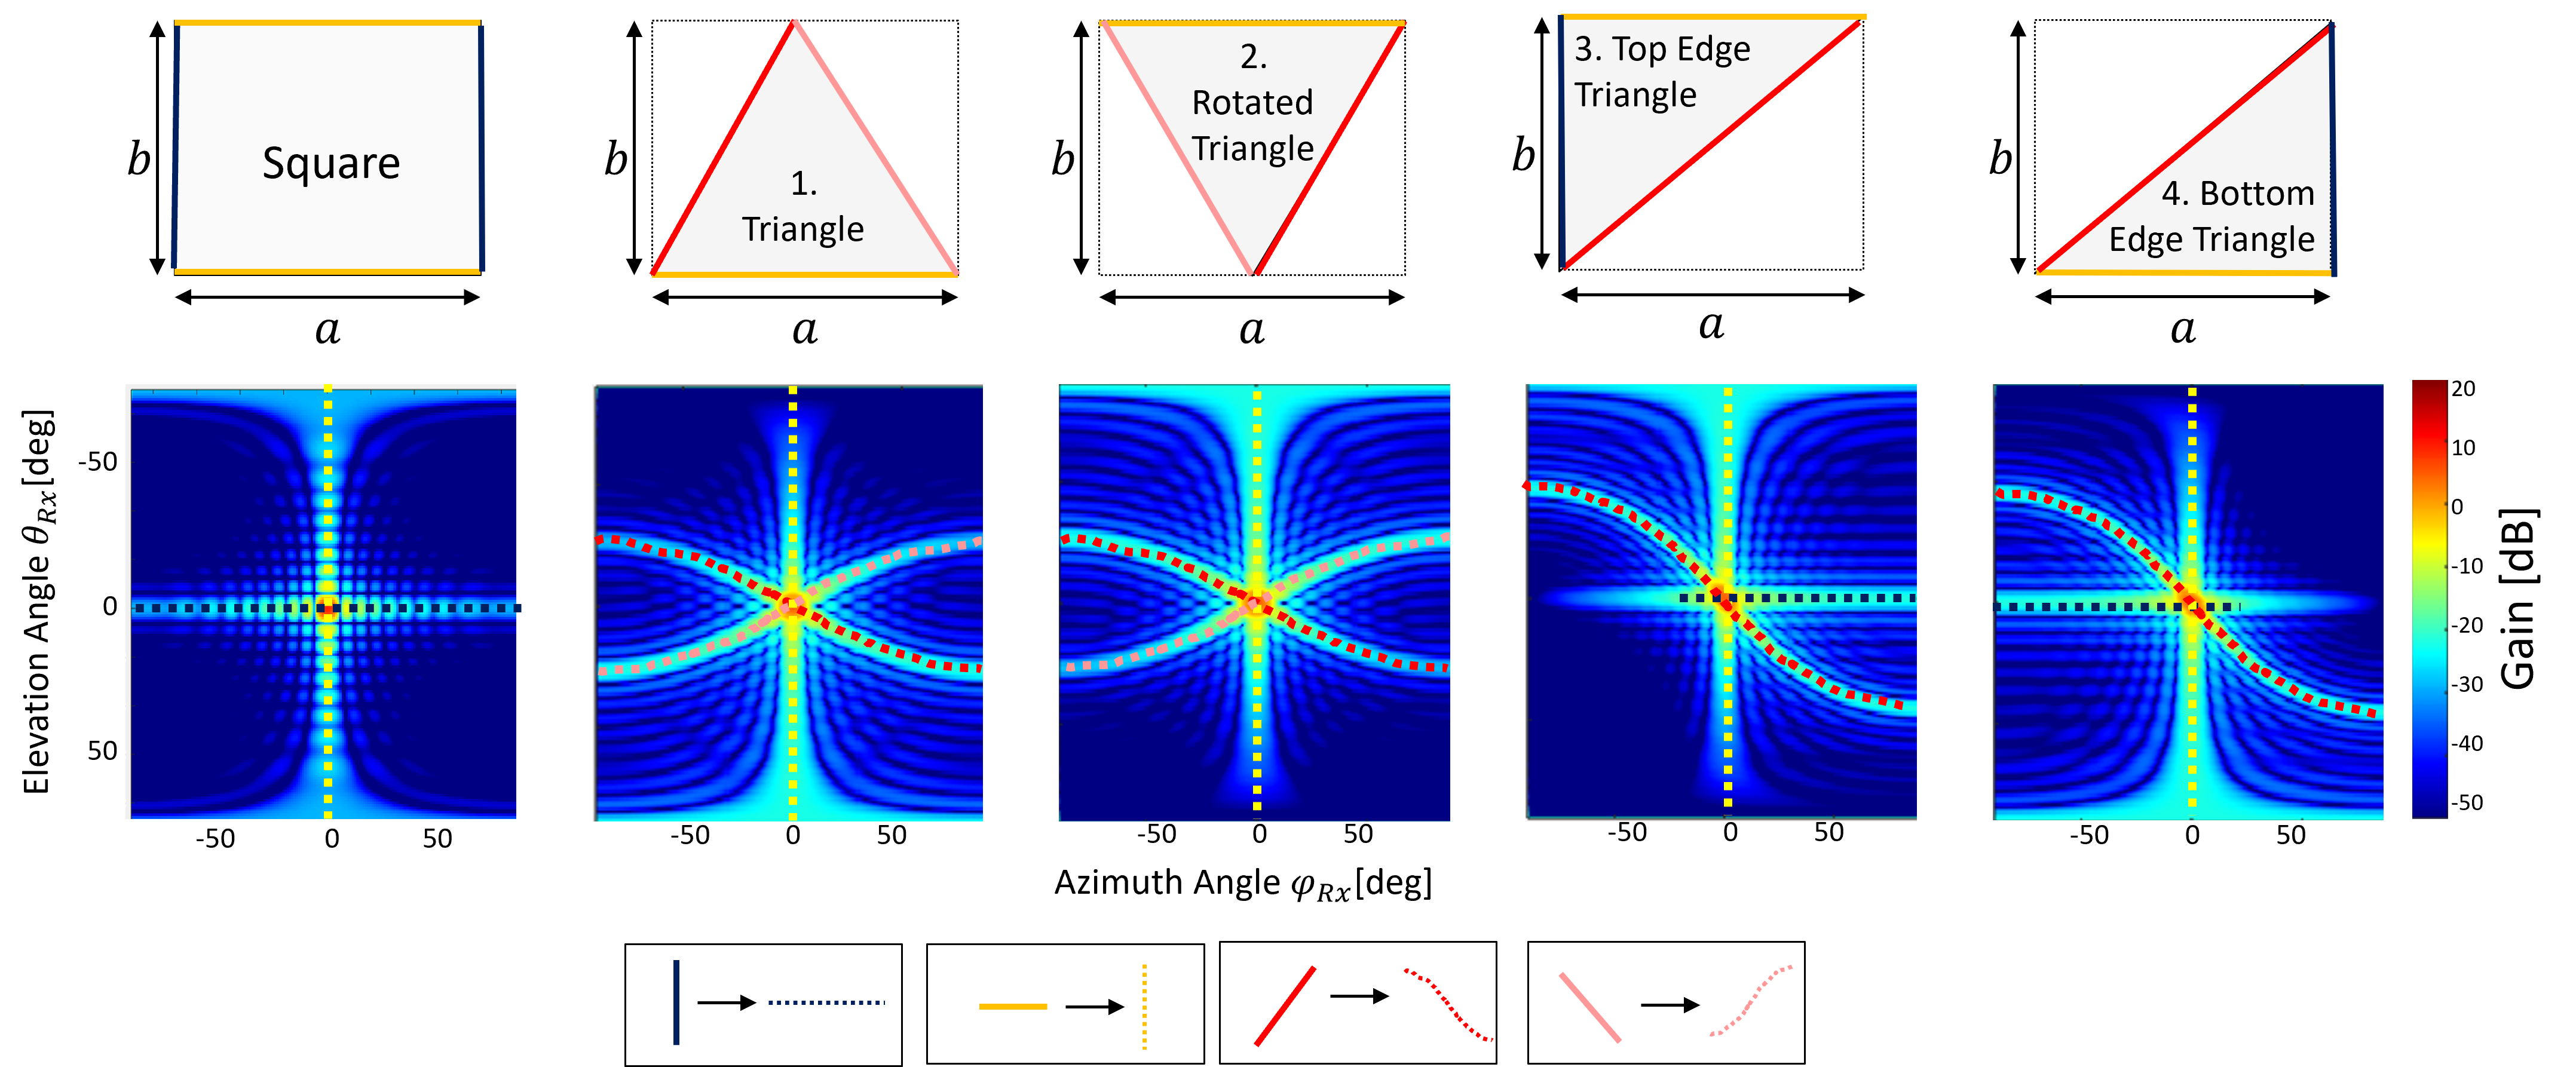
\includegraphics[width=1.0\linewidth]{images/Section 4 Images/Triangle_square}
	\caption{Illustration of the squared and triangle geometry models with different triangular orientations with their RCS behavior depicting the gain in \si{\decibel}. Assuming the flat plate geometry with $\varphi_{Tx}=\theta_{Tx}=0^\circ$, the color coding on the geometry of square and triangle can be seen on the RCS heatmap, denoting the impact of the different sides of the geometry on the RCS behavior, which is the same for various orientations of the triangular plate.}
	\label{fig:Triangle_square}
\end{figure}
parallel to the $y$-axis, and red and peach when in the $y$-$z$-plane with a rising or falling gradient. In the middle of the figure, we present the arising RCS heatmaps given a \SI{28}{\giga\hertz} incident wave from direction $\varphi_{Tx}=\theta_{Tx}=0^\circ$. Interestingly, the four different triangles exhibit unique RCS patterns, although there are similarities with the RCS pattern of the square-shaped surface patch on the left if the respective triangle also contains an edge along the y-axis (black), and x-axis (yellow). The best match is for triangles number 3 and 4, which feature both a black and a yellow edge. Here we see that the red edge must be the reason why a diagonal-like pattern arises in the RCS pattern.  

\begin{figure}[tb]
	\centering
	\subfloat[Variation of peak gain in $\si{\decibel}$ for the sweep along the elevation angle $\theta_{Tx}$ when $\varphi_{Tx}=0^\circ$. A notable difference of \SI{6}{\decibel} is observed at $\varphi_{Tx}=\theta_{Tx}=0^\circ$ for triangle number 1 in \Cref{fig:Triangle_square}. The other triangles yield the same result as this.]{
		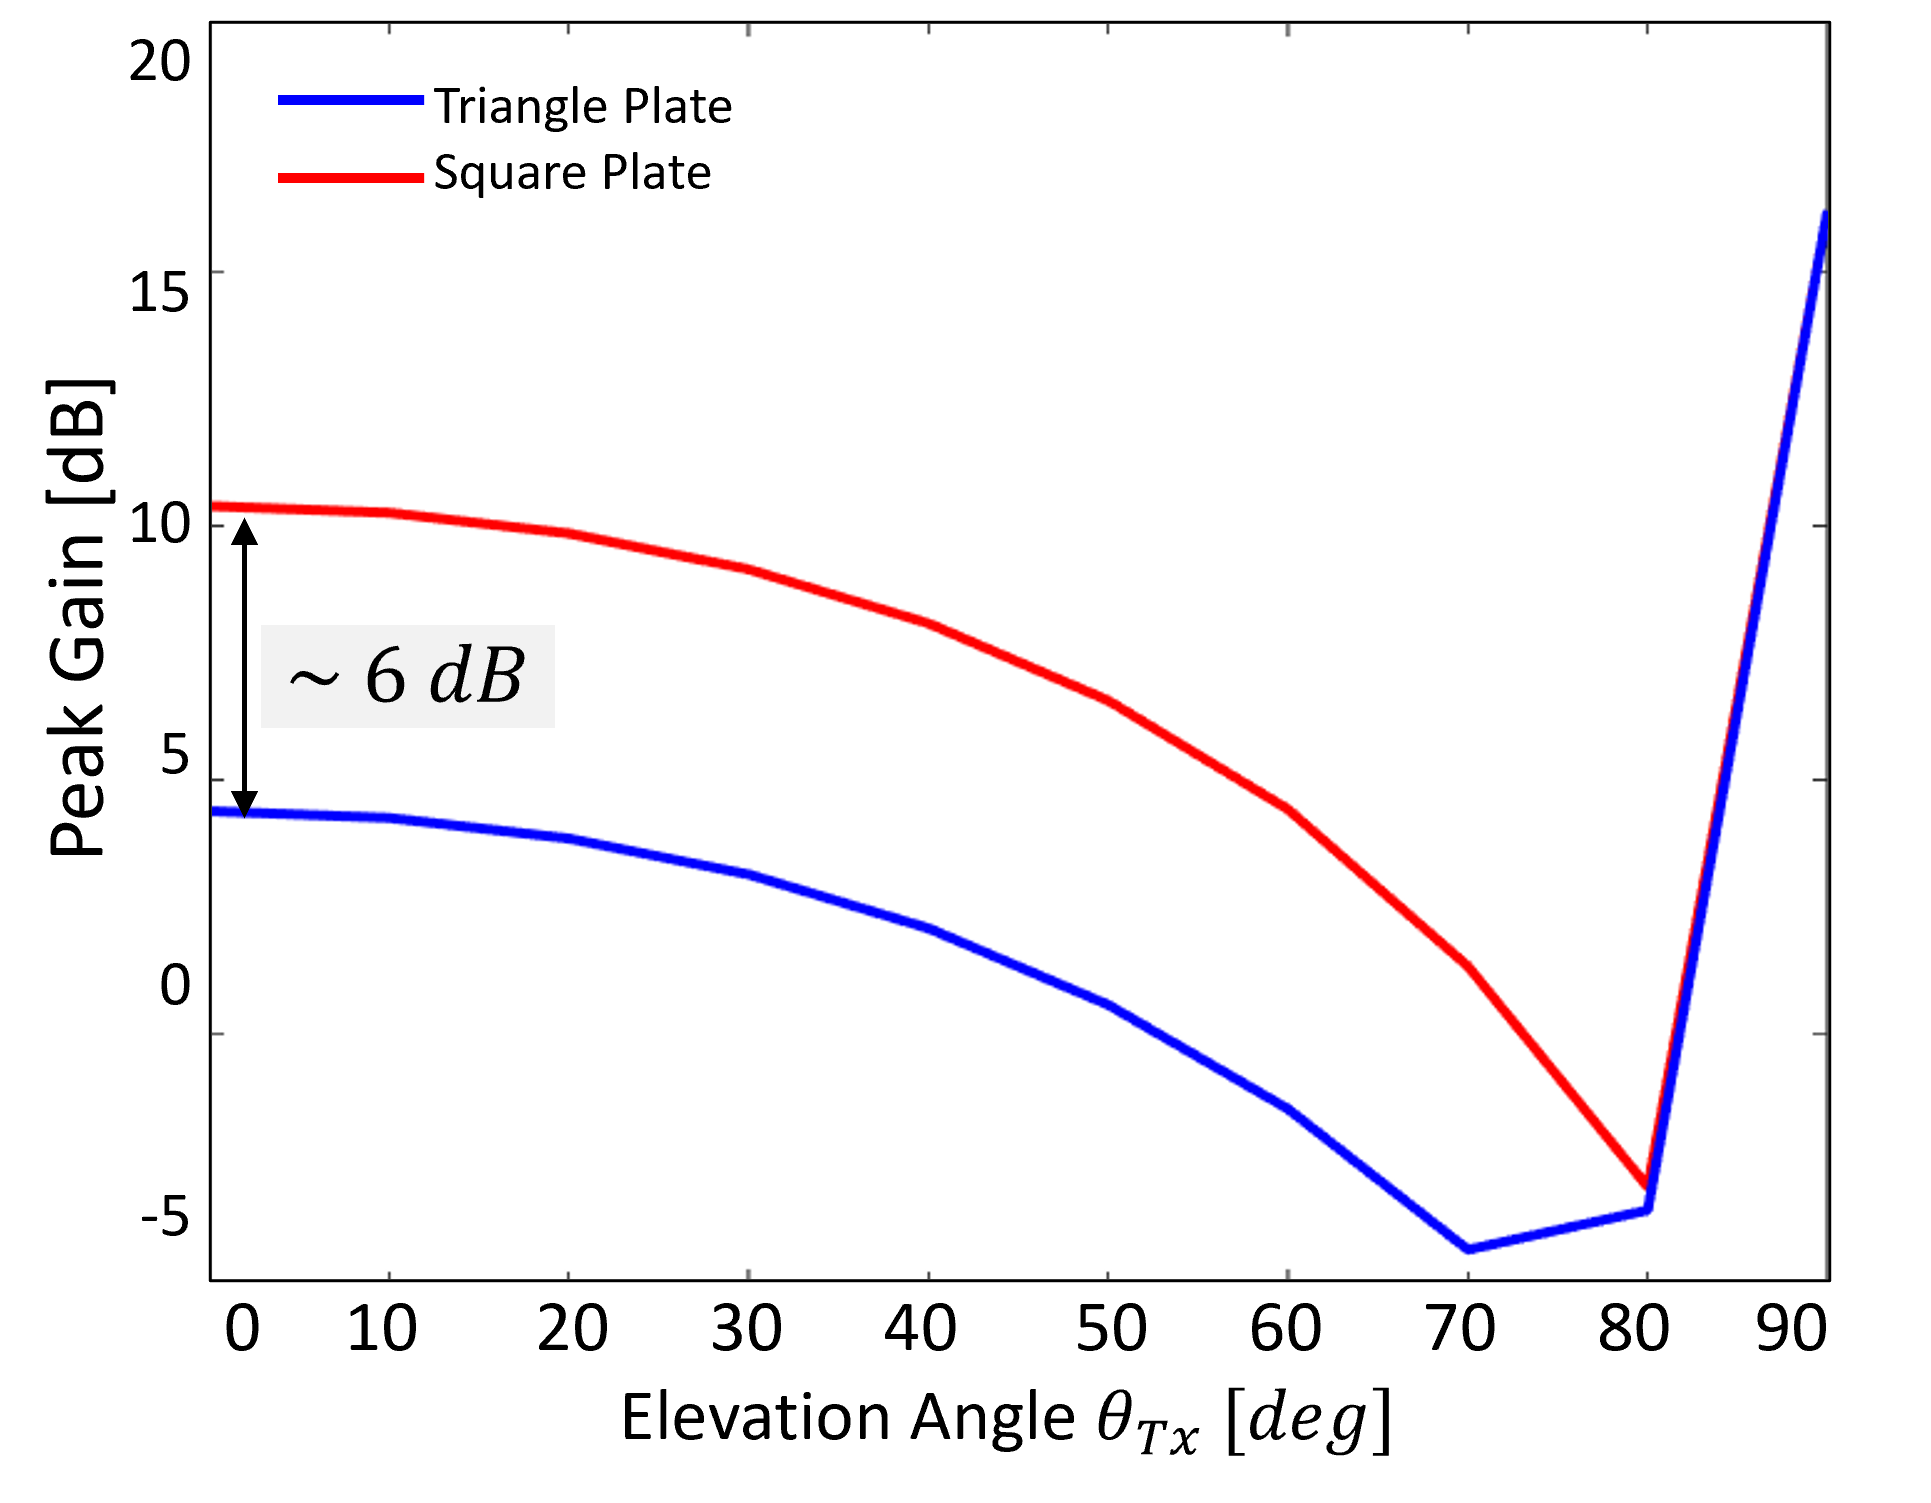
\includegraphics[width=0.31\linewidth]{images/Section 4 Images/Triangle_square_compare_1}
			\label{fig:Triangle_square_compare1}
	}
		\hfill
	\subfloat[Gain behavior in \si{\decibel} when plotted against elevation angle $\theta_{Rx}$, observing a \SI{6}{\decibel} decrease in the gain from that of rectangle plate considering triangle number 1 in \Cref{fig:Triangle_square}.]{
		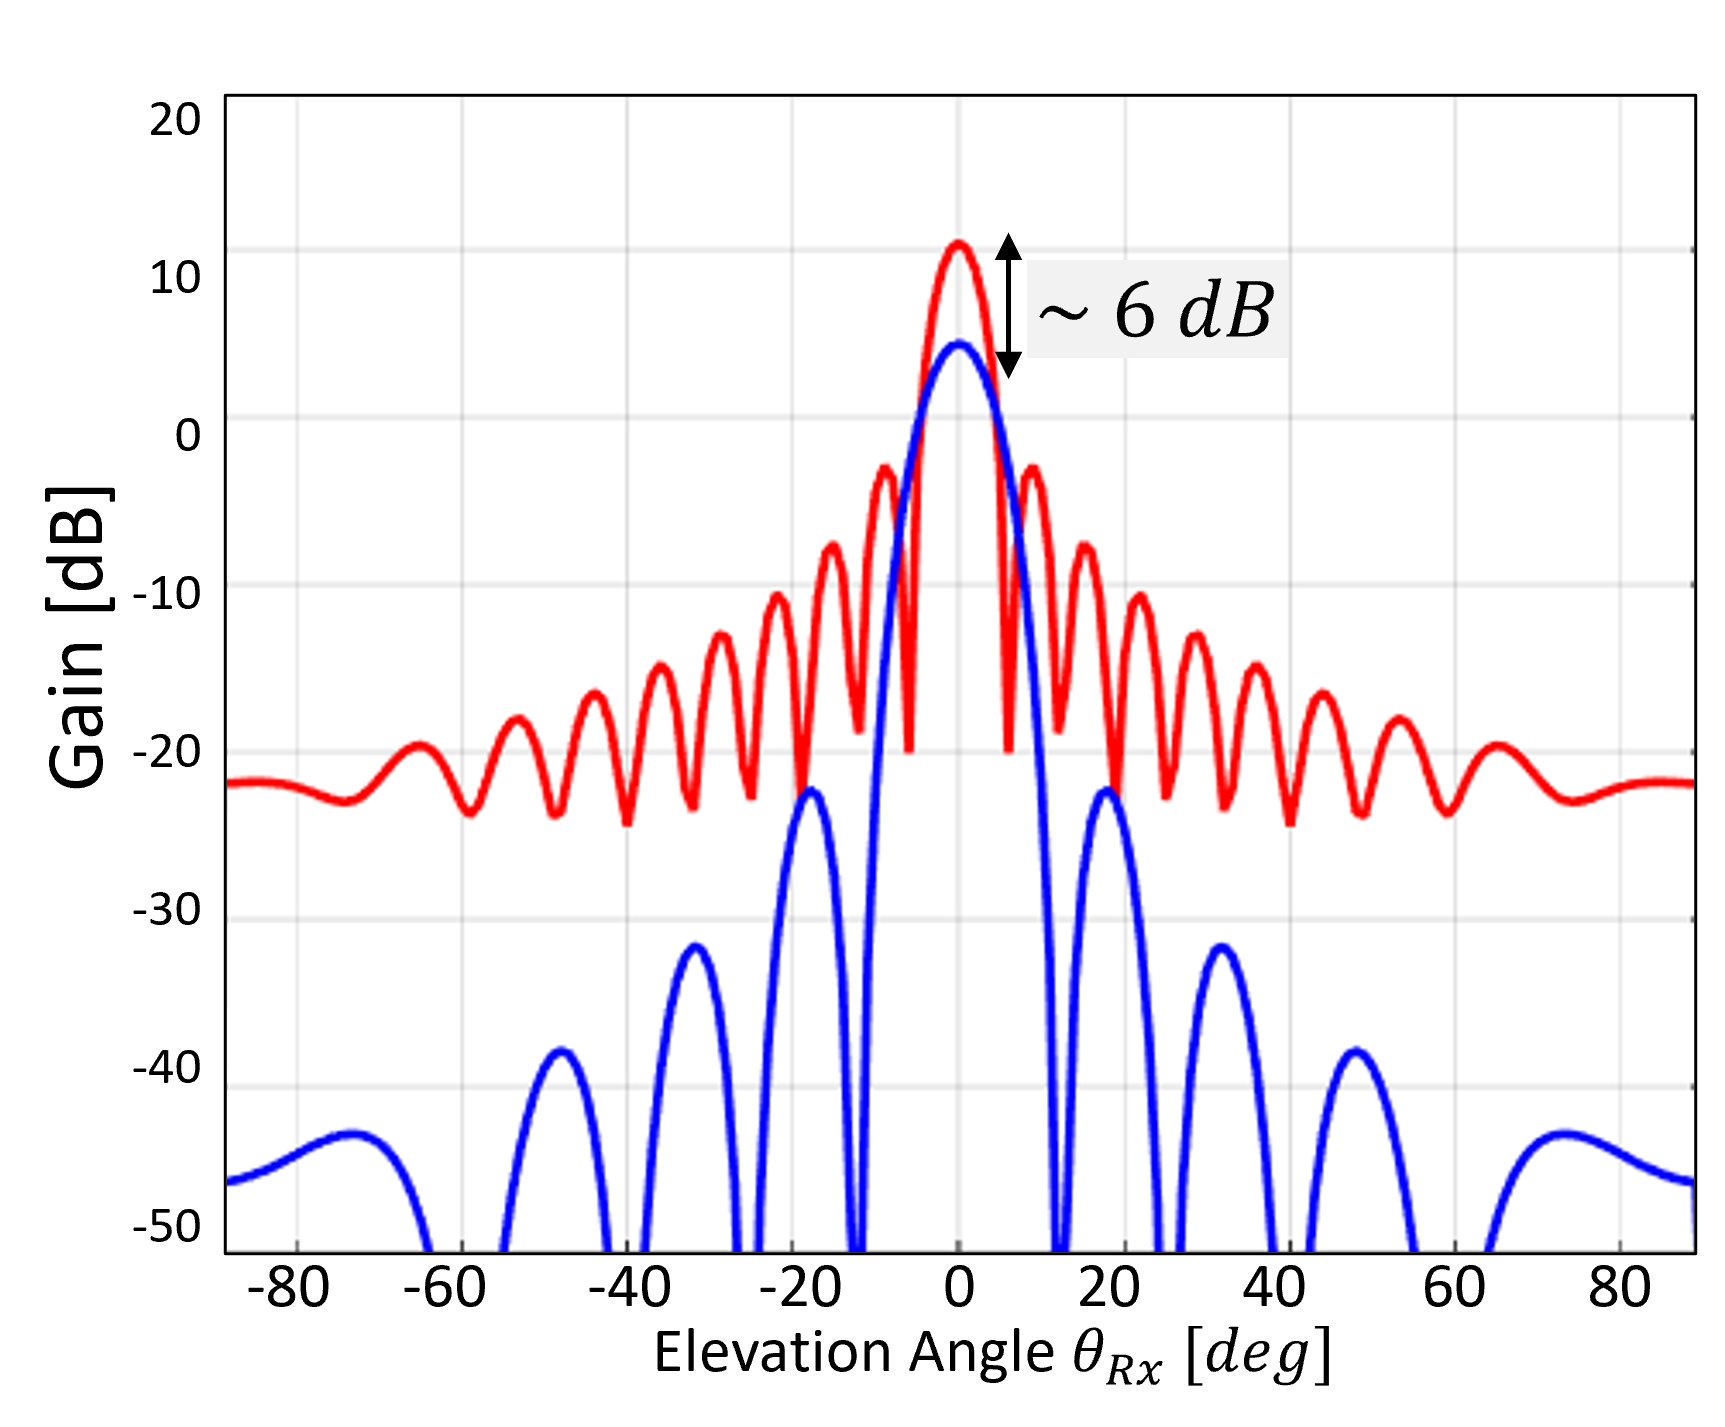
\includegraphics[width=0.31\textwidth]{images/Section 4 Images/Triangle_square_compare}
		\label{fig:trisuq1}
	}
		\hfill
	\subfloat[Gain behavior in \si{\decibel} when plotted against elevation angle $\theta_{Rx}$. The RCS "summation" of triangle numbers 3 and 4 in \Cref{fig:Triangle_square} leads to a black curve, where we observe a \SI{1.5}{\decibel} decrease in the gain from that of the rectangle plate.]{
		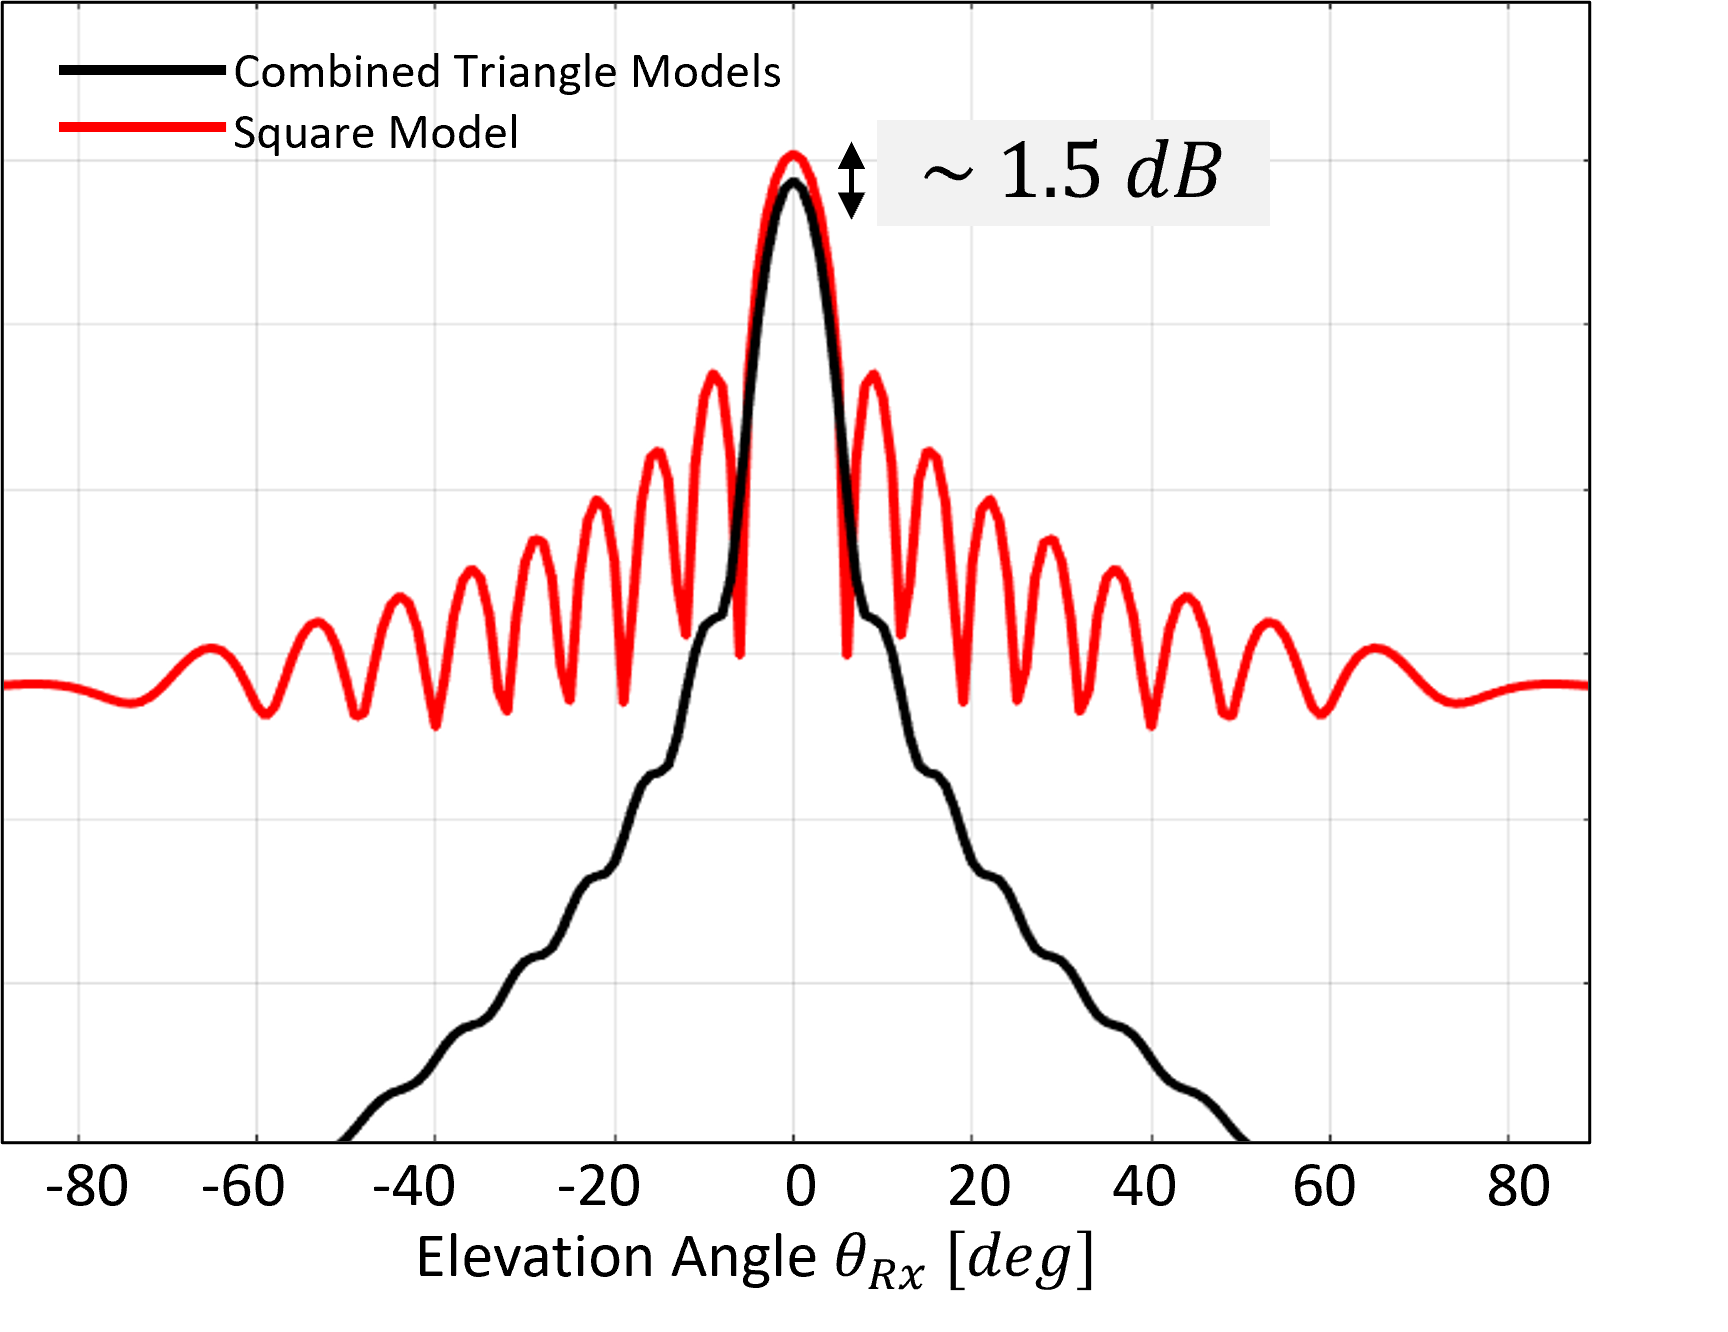
\includegraphics[width=0.31\textwidth]{images/Section 4 Images/TogetherTriangle_square_compare}
		\label{fig:trisuq2}
	}
	\caption[Gain behavior in \si{\decibel} for the rectangle and triangle plate when $a=b=\SI{0.1}{\meter}$, and $\varphi_{Tx}=\theta_{Tx}=0^\circ$. The main difference between the two plates is with their areas, due to which we observe \SI{6}{\decibel} between these models as depicted.]{Gain behavior in \si{\decibel} for the rectangle and triangle plate when $a=b=\SI{0.1}{\meter}$, and $\varphi_{Tx}=\theta_{Tx}=0^\circ$. The main difference between the two plates are is their areas, due to which we observe \SI{6}{\decibel} between these models as depicted.}
	\label{fig:trisuq}
\end{figure}
Due to this, we can also conclude that the peach-colored edge must be the origin for the 180° rotated diagonal-like pattern in the RCS. As such we concluded that an analytical model of the RCS pattern needs to factor in the orientation of the edges, respectively, to recreate such patterns.

Fixing $\varphi_{Tx}=0^\circ$, \Cref{fig:Triangle_square_compare1} explores the peak RCS along different $\theta_{Tx}$ in the range from $[0: 90]^\circ$. We observe a \SI{6}{\decibel} difference for $\theta_{Tx}=0^\circ$, as expected from our earlier consideration. For larger $\theta_{Tx}$, the difference mitigates. This is because the main lobe changes and $\sigma_{Tri}$ outside of the main lobe depends not only on $A_{tri}^2$ but also strongly on $\varphi_{Tx}, \theta_{Tx}, \varphi_{Rx}$, and $\theta_{Rx}$.

As can be seen from \Cref{fig:trisuq1} and \Cref{fig:trisuq2}, a different beamwidth pattern occurs for triangle and rectangle surfaces. Referring to \Cref{fig:Triangle_square} again, the RCS "summation" of the final two triangles, using \Cref{Eq:RCS_SUMMATION}, is now compared in \Cref{fig:trisuq2} to the RCS of the equivalent square-shaped reflecting surface. We observe that the main lobe peak differs by approx. \SI{1.5}{\decibel}, however, the form of the mainlobe matches nicely. We further find that the RCS patterns from two triangles are not able to represent the sidelobes of the rectangle accurately.

This outlines that RCS patterns of arbitrary complex geometries represented using triangles may be prone to errors, particularly in the sidelobe region, Nonetheless, it is important to note that the main lobe is still accurate such that a potential analytical model may still be used with sufficient accuracy to assess the performance in the intended reflection direction of the reflector.